\documentclass[twoside,11pt]{article} % For LaTeX2e
\usepackage{jmlr2e}
\usepackage{hyperref}
\hypersetup{colorlinks,
            urlcolor=blue,
            citecolor=green,
            linkcolor=red}
\usepackage{url}
%\documentstyle[nips13submit_09,times,art10]{article} % For LaTeX 2.09
\usepackage{mathrsfs}
%\usepackage{amsthm}
\usepackage{amsmath}
\usepackage{amsfonts}
%\usepackage{amssymb}
\usepackage{algorithmic}
\usepackage{algorithm}
\usepackage{color}
\usepackage{mathtools}

\usepackage{pstricks}
\usepackage{tikz}
\usepackage{subcaption}

\newcommand{\fix}{\marginpar{FIX}}
\newcommand{\new}{\marginpar{NEW}}

% Misc. math commands.  I couldn't figure out how to make the Unicode cat
% character, sadly.
\newcommand{\argmax}{\operatornamewithlimits{argmax}}
\newcommand{\var}{\operatorname{var}}

\newcommand{\K}{\mathcal{K}}
\newcommand{\hilbert}{\mathcal{H}}
\newcommand{\Real}{\mathcal{R}}

\renewcommand{\algorithmicforall}{\textbf{for each}}
\renewcommand{\algorithmicrepeat}{\textbf{do}}
\renewcommand{\algorithmicuntil}{\textbf{while}}

%\newtheorem{defn}{Definition}
%\newtheorem{thm}{Theorem}
%\newtheorem{lemma}{Lemma}
%\newtheorem{cor}{Corollary}
\newtheorem{defn}{Definition}
\newtheorem{thm}{Theorem}
\newtheorem{cor}{Corollary}


\begin{document}

\title{Plug-and-play dual-tree algorithm runtime analysis}

\author{\name Ryan R. Curtin \email ryan@ratml.org\\
  \addr School of Computational Science and Engineering\\
  Georgia Institute of Technology\\
  Atlanta, GA 30332-0250, USA
  \AND
  \name Dongryeol Lee \email drselee@gmail.com\\
  \addr GE Research\\
  Schenedectadadaty, NY\\
  \AND
  \name William B. March \email march@ices.utexas.edu\\
  \addr Austin, TX, USA\\
  \AND
  \name Parikshit Ram \email p.ram@gatech.edu\\
  \addr Skytree
}

\editor{Unknown}

\maketitle

\begin{abstract}
%A large collection of machine learning algorithms contain subproblems that can
%be efficiently solved with trees.  In the situation where a dual-tree algorithm
%with cover trees is used to solve a problem, rigorous worst-case runtime bounds
%can often be shown.  A worst-case runtime bound is proven for all cover tree
%dual-tree algorithms; this bound can be employed to give useful runtime bounds
%for individual problems.  We show a new, tighter bound of $O(c^9 \nu N)$ for
%all-nearest-neighbor search and also provide linear runtime bounds for
%approximate kernel density estimation and exact range count/search under some
%mild assumptions.  These are the first linear runtime bounds we are aware of for
%range count/search.
%Numerous machine learning algorithms contain pairwise statistical problems at
%their core. Often, tree structures are used to solve these problems efficiently.
%Dual-tree algorithms using cover trees have rigorous worst-case runtime
%guarantees for some of these problems. In this paper, we present a {\em
%problem-independent} runtime guarantee for {\em any} dual-tree algorithm using
%the cover tree, separating out the problem-dependent and the problem-independent
%elements. This allows us to just plug in bounds for the problem-dependent
%elements to get runtime guarantees for dual-tree algorithms for any pairwise
%statistical problem. We demonstrate this plug-and-play procedure for
%nearest-neighbor search and approximate kernel density estimation to get
%improved runtime guarantees.  Under some assumptions, we also present the first
%linear runtime guarantee for dual-tree based range search.
Numerous machine learning algorithms contain pairwise statistical problems at
their core -- i.e. tasks that require computations over all pairs of input points if implemented directly. 
Often, tree structures are used to solve these problems efficiently. Dual-tree algorithms 
can efficiently solve or approximate many of these problems.
Using cover trees, rigorous worst-case runtime
guarantees have been proven for some of these algorithms. In this paper, we present a {\em
problem-independent} runtime guarantee for {\em any} dual-tree algorithm using
the cover tree, separating out the problem-dependent and the problem-independent
elements. This allows us to plug in bounds for the problem-dependent
elements to get runtime guarantees for dual-tree algorithms for any pairwise
statistical problem without re-deriving the entire proof. We demonstrate this plug-and-play procedure for
nearest-neighbor search and approximate kernel density estimation to get
improved runtime guarantees.  Under mild assumptions, we also present the first
linear runtime guarantee for dual-tree based range search.
\end{abstract}


\section{Dual-tree algorithms}

A surprising number of machine learning algorithms have computational
bottlenecks that can be expressed as pairwise statistical problems. 
By this, we mean computational tasks that can be evaluated directly by iterating over all 
pairs of input points. 
Nearest neighbor search is one such problem, since for every query point, we can 
evaluate its distance to every reference point and keep the closest one. 
This naively requires $O(N)$ time
to answer in single query in a reference set of size $N$; answering $O(N)$
queries subsequently requires prohibitive $O(N^2)$ time. Kernel density
estimation is also a pairwise statistical problem, since we compute a sum over all 
reference points for each query point.
This again requires $O(N^2)$
time to answer $O(N)$ queries if done directly. 
The reference set is typically indexed with
spatial data structures to accelerate this type of computation
\citep{finkel1974quad, langford2006}; these result in $O(\log N)$ runtime per
query under favorable conditions.

\citet{nbody} generalized the fast multipole method from
computational physics to obtain dual-tree algorithms.  These are extremely
useful when there are large query sets, not just a few query points.  Instead of
building a tree on the reference set and searching with each query point
separately, Gray and Moore suggest also building a query tree and traversing
both the query and reference trees simultaneously (a {\it dual-tree traversal},
from which the class of algorithms takes its name).

Dual-tree algorithms can be easily understood through the recent framework of
\citet{curtin2013tree}: two trees (a query tree and a reference
tree) are traversed by a {\it pruning dual-tree traversal}.  This traversal
visits combinations of nodes from the trees in some sequence (each combination
consisting of a query node and a reference node), calling a problem-specific
\texttt{Score()} function to determine if the node combination can be pruned.
If not, then a problem-specific \texttt{BaseCase()} function is called for each
combination of points held in the query node and reference node.  This has
significant similarity to the more common single-tree branch-and-bound
algorithms, except that the algorithm must recurse into child nodes of {\it
both} the query tree and reference tree.

There exist numerous dual-tree algorithms for problems as diverse as kernel
density estimation \citep{gray2003nonparametric}, mean shift \citep{wang2007fast},
minimum spanning tree calculation \citep{march2010euclidean}, $n$-point
correlation function estimation \citep{march2012fast}, max-kernel search
\citep{curtin2013fast}, particle smoothing \citep{klaas2006fast}, variational
inference \citep{amizadeh2012variational}, and range search \citep{nbody}, to name
a few.

Some of these algorithms are derived using the cover tree \citep{langford2006}, a
data structure with beneficial theoretical qualities.  Dual-tree all
nearest-neighbor search and approximate kernel density estimation with cover
trees have $O(N)$ runtime guarantees for $O(N)$ queries \citep{ram2009}; minimum
spanning tree calculation scales as $O(N \log N)$ \citep{march2010euclidean}.
Other problems have similar worst-case guarantees \citep{curtin2014dual,
march2013multi}.

In this work we combine the generalization of \citet{curtin2013tree} with the
theoretical results of \citet{langford2006} and others in order to develop a
worst-case runtime bound for any dual-tree algorithm when the cover tree is
used.

Section \ref{sec:preliminaries} lays out the required background, notation, and
introduces the cover tree and its associated theoretical properties.  Readers
familiar with the cover tree literature and dual-tree algorithms
\citep[especially][]{curtin2013tree} may find that section to be review.
Following that, we introduce an intuitive measure of cover tree imbalance, an 
important property for understanding the runtime of dual-tree algorithms, in
Section \ref{sec:imbalance}.  This measure of imbalance is then used to prove
the main result of the paper in Section \ref{sec:bound}, which is a worst-case
runtime bound for generalized dual-tree algorithms.  We apply this result to
three specific problems: nearest neighbor search (Section \ref{sec:nns}),
approximate kernel density estimation (Section \ref{sec:akde}), and range search
/ range count (Section \ref{sec:rs}), showing linear runtime bounds for each of
those algorithms.  Each of these bounds is an improvement on the
state-of-the-art, and in the case of range search, is the first such bound.
%  We
%then investigate the empirical performance of cover trees for these algorithms
%in Section \ref{sec:emp}, with a focus on understanding the dataset-dependent
%constants that our bounds use.

\section{Preliminaries}
\label{sec:preliminaries}

For simplicity, the algorithms considered in this paper will be presented in a
tree-independent context, as in \citet{curtin2013tree}, but the only type of
tree we will consider is the cover tree \citep{langford2006}, and the only type
of traversal we will consider is the cover tree pruning dual-tree traversal,
which we will describe below.

As we will be making heavy use of trees, we must establish notation \citep[taken
from][]{curtin2013tree}.  The notation we will be using is defined in Table
\ref{tab:notation}.

\begin{table}
{\small
\begin{center}
\begin{tabular}{|c|l|}
\hline
{\bf Symbol} & {\bf Description} \\ \hline
$\mathscr{N}$ & A tree node \\ \hline
$\mathscr{C}_i$ & Set of child nodes of $\mathscr{N}_i$ \\ \hline
$\mathscr{P}_i$ & Set of points held in $\mathscr{N}_i$ \\ \hline
$\mathscr{D}_i^n$ & Set of descendant nodes of $\mathscr{N}_i$ \\ \hline
$\mathscr{D}_i^p$ & Set of points contained in $\mathscr{N}_i$ and
$\mathscr{D}_i^n$ \\ \hline
$\mu_i$ & Center of $\mathscr{N}_i$ (for cover trees, $\mu_i = p_i$) \\ \hline
$\lambda_i$ & Furthest descendant distance \\ \hline
\end{tabular}
\end{center}
}
\caption{Notation for trees.  See \cite{curtin2013tree} for details.}
\label{tab:notation}
\end{table}

The cover tree is a leveled hierarchical data structure originally proposed for
the task of nearest neighbor search.  The original description of the tree
describes both an {\it implicit} and {\it explicit} representation, where the
explicit representation is the actual structure that would be implemented in
practice.  Thus, we will consider only the explicit representation in this
paper.

Each node $\mathscr{N}_i$ in the cover tree is indexed by an integer scale $s_i$
and holds one point $p_i$ which is also the center of the node ($p_i = \mu_i$).
The cover tree node may have a number of child nodes; if the cover tree node
does have children, then one child will be the self-child, which holds the same
point $p_i$ with a smaller scale $s_i$.  Each child of $\mathscr{N}_i$ will have
scale less than $s_i$, and every descendant point of a node $\mathscr{N}_i$
(that is, the set $\mathscr{D}_i^p$) has a maximum distance of $2^{s_i + 1}$
from the point $p_i$.

Assuming a cover tree $\mathscr{T}$ is built on a dataset $S_r$, let $C_{s_i}$
denote the set of points held in all nodes in $\mathscr{T}$ with scale $s_i$.
Then, the cover tree satisfies the following invariants for all scales $s_i$:

\begin{itemize}

\item {\em (Nesting)}.  $C_{s_i} \subset C_{s_i - 1}$.  This means that when a
point $p_i \in S_r$ is held in a node at some scale $s_i$, then each smaller
scale will also have a node containing $p_i$.

\item {\em (Covering tree)}.  For every point $p_i \in C_{s_i - 1}$, there
exists a point $p_j \in C_{s_i}$ such that $d(p_i, p_j) < 2^{s_i}$, and the node
holding $p_j$ with scale $s_i$ is the parent node of the node holding $p_i$ with
scale $s_i - 1$.

\item {\em (Separation)}.  For all distinct points $p_i, p_j \in C_{s_i}$,
$d(p_i, p_j) > 2^{s_i}$.

\end{itemize}

A batch construction algorithm is given by \citet{langford2006}, called
\texttt{Construct}; but the details of construction are not relevant to our
work, so we only mention this as a reference.  More relevant to our work is the
number of useful and unique theoretical properties the cover tree possesses,
based on the expansion constant \citep{karger2002finding}; we restate the
definition below.

\begin{defn}
\label{def:int_dim}
Let $B_S(p, \Delta)$ be the set of points in $S$ within a closed ball of radius
$\Delta$ around some $p \in S$ with respect to a metric $d$:
%
$B_S(p, \Delta) = \{ r \in S \colon d(p, r) \leq \Delta \}$.
%
Then, the {\bf expansion constant} of $S$ with respect to the metric $d$ is the
smallest $c \ge 2$ such that

\begin{equation}
| B_S(p, 2 \Delta) | \le c | B_S(p, \Delta) |\ \forall\ p \in S,\
\forall\ \Delta > 0.
\end{equation}

\end{defn}

The expansion constant is used heavily in the cover tree literature.  It is
related to a notion of instrinic dimensionality, and previous work has shown
that there are many scenarios where $c$ is independent of the number of points
in the dataset.

The expansion constant can be used to show a few useful bounds on various
properties of the cover tree; we restate these results below, given some cover
tree built on a dataset $S$ with expansion constant $c$ and $|S| = N$:

\begin{itemize}
  \item {\bf Width bound:} no cover tree node has more than $c^4$ children
(Lemma 4.1, \cite{langford2006}).

  \item {\bf Depth bound:} the maximum depth of any node is $O(c^2 \log N)$
(Lemma 4.3, \cite{langford2006}).

  \item {\bf Space bound:} a cover tree has $O(N)$ nodes (Theorem 1,
\cite{langford2006}).
\end{itemize}

%\begin{lemma}
%\label{lem:width}
%(Lemma 4.1, \cite{langford2006}) The number of children of any cover tree node $\mathscr{N}_i$ is bounded by
%$c^4$, where $c$ is the expansion constant of the dataset the cover tree is
%built on, as defined in Definition \ref{def:int_dim}.
%\end{lemma}

%\begin{lemma}
%\label{lem:depth}
%(Lemma 4.3, \cite{langford2006}) The maximum depth of any point $p_r$ in a cover
%tree $\mathscr{T}_r$ is $O(c^2 \log N)$, where $N$ is the number of points in
%the dataset that $\mathscr{T}_r$ is built on.
%\end{lemma}

Lastly, we introduce a convenience lemma of our own which is a generalization of
the packing arguments used by \citet{langford2006}.  This is a more flexible
version of their argument.

\begin{lemma}
Consider a dataset $S$ with expansion constant $c$ and a subset $C \subseteq S$
such that every point in $C$ is separated by $\delta$.  Then, given any query
point $p \not\in S$ and some radius $\rho \delta$,

\begin{equation}
| B_S(p, \rho \delta) \cap C | \le c^{2 + \log_2 \rho}.
\end{equation}
\label{lem:packing}
\end{lemma}

\begin{proof}
This is based on the packing argument from Lemma 4.1 in \cite{langford2006}.
Observe that $B_S(p, \rho \delta) \subseteq B_S(p_i, 2 \rho \delta)$ for any
$p_i \in S$, and that $| B_S(p, 2 \rho \delta) | = c^{2 + \log_2 \rho} |
B_S(p, \delta / 2) |$.  Because each point in $C$ is separated by $\delta$, the
number of points in $B_S(p, \rho \delta) \cap C$ is
bounded by the number of disjoint balls of radius $\delta / 2$ that can be
packed into $B_S(p, \rho \delta)$.  In the worst case, this packing is
perfect, and

\begin{equation}
|B_S(p, \rho \delta)| \le \frac{|B_S(p_i, 2 \rho \delta)|}{|B_S(p_i, \delta
/ 2)|} \le c^{2 + \log_2 \rho}.
\end{equation}
\end{proof}


\section{Tree imbalance}
\label{sec:imbalance}

It is well-known that imbalance in trees leads to degradation in performance;
for instance, a $kd$-tree node with every descendant except one in its left
child is effectively useless.  A $kd$-tree full of nodes like this will perform
abysmally for nearest neighbor search, and it is not hard to generate a dataset
that will cause a $kd$-tree of this sort.

This sort of imbalance applies to all types of trees, not just $kd$-trees.  In
our situation, we are interested in a better understanding of this imbalance for
cover trees, and thus endeavor to introduce a more formal measure of imbalance
which is correlated with tree performance.  Numerous measures of tree
imbalance have already been established; one example is that proposed by
\citet{colless1982review}, and another is Sackin's index \citep{sackin1972good},
but we aim to capture a different measure of imbalance that utilizes the leveled
structure of the cover tree.

We already know each node in a cover tree is indexed with an integer level (or
scale).  In the explicit representation of the cover tree, each non-leaf node
has children at a lower level.  But these children need not be strictly one
level lower; see Figure \ref{fig:imbalance}.  In Figure
\ref{fig:imbalance-good}, each cover tree node has children that are strictly
one level lower; we will refer to this as a {\em perfectly balanced cover tree}.
Figure \ref{fig:imbalance-bad}, on the other hand, contains the node
$\mathscr{N}_m$ which has two children with scale two less than $s_m$.  We will
refer to this as an {\em imbalanced cover tree}.  Note that in our definition,
the balance of a cover tree has nothing to do with differing number of
descendants in each child branch but instead only missing levels.

\begin{figure}
\begin{subfigure}[b]{0.585\textwidth}
  \begin{center}
    
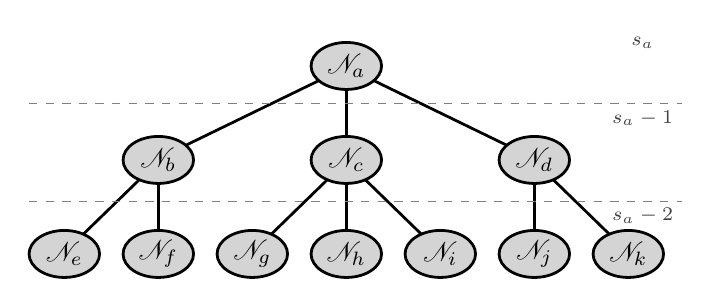
\begin{tikzpicture}[>=latex,line join=bevel,scale=0.47]
  \pgfsetlinewidth{1bp}
%%
\begin{scope}
  \pgfsetstrokecolor{black}
  \definecolor{strokecol}{rgb}{1.0,1.0,1.0};
  \pgfsetstrokecolor{strokecol}
  \definecolor{fillcol}{rgb}{1.0,1.0,1.0};
  \pgfsetfillcolor{fillcol}
  \filldraw (0bp,0bp) -- (0bp,180bp) -- (486bp,180bp) -- (486bp,0bp) -- cycle;
\end{scope}
\begin{scope}
  \pgfsetstrokecolor{black}
  \definecolor{strokecol}{rgb}{1.0,1.0,1.0};
  \pgfsetstrokecolor{strokecol}
  \definecolor{fillcol}{rgb}{1.0,1.0,1.0};
  \pgfsetfillcolor{fillcol}
  \filldraw (0bp,0bp) -- (0bp,180bp) -- (486bp,180bp) -- (486bp,0bp) -- cycle;
\end{scope}
\begin{scope}
  \pgfsetstrokecolor{black}
  \definecolor{strokecol}{rgb}{1.0,1.0,1.0};
  \pgfsetstrokecolor{strokecol}
  \definecolor{fillcol}{rgb}{1.0,1.0,1.0};
  \pgfsetfillcolor{fillcol}
  \filldraw (0bp,0bp) -- (0bp,180bp) -- (486bp,180bp) -- (486bp,0bp) -- cycle;
\end{scope}
  \pgfsetcolor{black}
  % Edge: c2 -> c6
  \draw [-] (228.43bp,74.834bp) .. controls (218.25bp,64.938bp) and (204.48bp,51.546bp)  .. (185.8bp,33.385bp);
  % Edge: c3 -> c9
  \draw [-] (387bp,71.697bp) .. controls (387bp,63.983bp) and (387bp,54.712bp)  .. (387bp,36.104bp);
  % Edge: c3 -> c10
  \draw [-] (401.57bp,74.834bp) .. controls (411.75bp,64.938bp) and (425.52bp,51.546bp)  .. (444.2bp,33.385bp);
  % Edge: c2 -> c8
  \draw [-] (257.57bp,74.834bp) .. controls (267.75bp,64.938bp) and (281.52bp,51.546bp)  .. (300.2bp,33.385bp);
  % Edge: c1 -> c4
  \draw [-] (84.43bp,74.834bp) .. controls (74.25bp,64.938bp) and (60.476bp,51.546bp)  .. (41.796bp,33.385bp);
  % Edge: c1 -> c5
  \draw [-] (99bp,71.697bp) .. controls (99bp,63.983bp) and (99bp,54.712bp)  .. (99bp,36.104bp);
  % Edge: root -> c1
  \draw [-] (221.75bp,150.67bp) .. controls (197.4bp,138.83bp) and (157.28bp,119.33bp)  .. (120.33bp,101.37bp);
  % Edge: root -> c2
  \draw [-] (243bp,143.7bp) .. controls (243bp,135.98bp) and (243bp,126.71bp)  .. (243bp,108.1bp);
  % Edge: c2 -> c7
  \draw [-] (243bp,71.697bp) .. controls (243bp,63.983bp) and (243bp,54.712bp)  .. (243bp,36.104bp);
  % Edge: root -> c3
  \draw [-] (264.25bp,150.67bp) .. controls (288.6bp,138.83bp) and (328.72bp,119.33bp)  .. (365.67bp,101.37bp);
  % Node: c7
\begin{scope}
  \definecolor{strokecol}{rgb}{0.0,0.0,0.0};
  \pgfsetstrokecolor{strokecol}
  \definecolor{fillcol}{rgb}{0.83,0.83,0.83};
  \pgfsetfillcolor{fillcol}
  \filldraw [opacity=1] (243bp,18bp) ellipse (27bp and 18bp);
  \draw (243bp,18bp) node {$\mathscr{N}_h$};
\end{scope}
  % Node: c9
\begin{scope}
  \definecolor{strokecol}{rgb}{0.0,0.0,0.0};
  \pgfsetstrokecolor{strokecol}
  \definecolor{fillcol}{rgb}{0.83,0.83,0.83};
  \pgfsetfillcolor{fillcol}
  \filldraw [opacity=1] (387bp,18bp) ellipse (27bp and 18bp);
  \draw (387bp,18bp) node {$\mathscr{N}_j$};
\end{scope}
  % Node: c8
\begin{scope}
  \definecolor{strokecol}{rgb}{0.0,0.0,0.0};
  \pgfsetstrokecolor{strokecol}
  \definecolor{fillcol}{rgb}{0.83,0.83,0.83};
  \pgfsetfillcolor{fillcol}
  \filldraw [opacity=1] (315bp,18bp) ellipse (27bp and 18bp);
  \draw (315bp,18bp) node {$\mathscr{N}_i$};
\end{scope}
  % Node: c3
\begin{scope}
  \definecolor{strokecol}{rgb}{0.0,0.0,0.0};
  \pgfsetstrokecolor{strokecol}
  \definecolor{fillcol}{rgb}{0.83,0.83,0.83};
  \pgfsetfillcolor{fillcol}
  \filldraw [opacity=1] (387bp,90bp) ellipse (27bp and 18bp);
  \draw (387bp,90bp) node {$\mathscr{N}_d$};
\end{scope}
  % Node: c2
\begin{scope}
  \definecolor{strokecol}{rgb}{0.0,0.0,0.0};
  \pgfsetstrokecolor{strokecol}
  \definecolor{fillcol}{rgb}{0.83,0.83,0.83};
  \pgfsetfillcolor{fillcol}
  \filldraw [opacity=1] (243bp,90bp) ellipse (27bp and 18bp);
  \draw (243bp,90bp) node {$\mathscr{N}_c$};
\end{scope}
  % Node: c1
\begin{scope}
  \definecolor{strokecol}{rgb}{0.0,0.0,0.0};
  \pgfsetstrokecolor{strokecol}
  \definecolor{fillcol}{rgb}{0.83,0.83,0.83};
  \pgfsetfillcolor{fillcol}
  \filldraw [opacity=1] (99bp,90bp) ellipse (27bp and 18bp);
  \draw (99bp,90bp) node {$\mathscr{N}_b$};
\end{scope}
  % Node: c10
\begin{scope}
  \definecolor{strokecol}{rgb}{0.0,0.0,0.0};
  \pgfsetstrokecolor{strokecol}
  \definecolor{fillcol}{rgb}{0.83,0.83,0.83};
  \pgfsetfillcolor{fillcol}
  \filldraw [opacity=1] (459bp,18bp) ellipse (27bp and 18bp);
  \draw (459bp,18bp) node {$\mathscr{N}_k$};
\end{scope}
  % Node: root
\begin{scope}
  \definecolor{strokecol}{rgb}{0.0,0.0,0.0};
  \pgfsetstrokecolor{strokecol}
  \definecolor{fillcol}{rgb}{0.83,0.83,0.83};
  \pgfsetfillcolor{fillcol}
  \filldraw [opacity=1] (243bp,162bp) ellipse (27bp and 18bp);
  \draw (243bp,162bp) node {$\mathscr{N}_a$};
\end{scope}
  % Node: c6
\begin{scope}
  \definecolor{strokecol}{rgb}{0.0,0.0,0.0};
  \pgfsetstrokecolor{strokecol}
  \definecolor{fillcol}{rgb}{0.83,0.83,0.83};
  \pgfsetfillcolor{fillcol}
  \filldraw [opacity=1] (171bp,18bp) ellipse (27bp and 18bp);
  \draw (171bp,18bp) node {$\mathscr{N}_g$};
\end{scope}
  % Node: c5
\begin{scope}
  \definecolor{strokecol}{rgb}{0.0,0.0,0.0};
  \pgfsetstrokecolor{strokecol}
  \definecolor{fillcol}{rgb}{0.83,0.83,0.83};
  \pgfsetfillcolor{fillcol}
  \filldraw [opacity=1] (99bp,18bp) ellipse (27bp and 18bp);
  \draw (99bp,18bp) node {$\mathscr{N}_f$};
\end{scope}
  % Node: c4
\begin{scope}
  \definecolor{strokecol}{rgb}{0.0,0.0,0.0};
  \pgfsetstrokecolor{strokecol}
  \definecolor{fillcol}{rgb}{0.83,0.83,0.83};
  \pgfsetfillcolor{fillcol}
  \filldraw [opacity=1] (27bp,18bp) ellipse (27bp and 18bp);
  \draw (27bp,18bp) node {$\mathscr{N}_e$};
\end{scope}
%
\draw[gray,thin,dashed] (0bp,58bp) -- (500bp,58bp);
\draw[gray,thin,dashed] (0bp,133bp) -- (500bp,133bp);

\draw (470bp,180bp) node[darkgray] {\scriptsize $s_a$};
\draw (470bp,122bp) node[darkgray] {\scriptsize $s_a - 1$};
\draw (470bp,47bp) node[darkgray] {\scriptsize $s_a - 2$};
\end{tikzpicture}


  \end{center}
  \caption{Balanced cover tree.}
  \label{fig:imbalance-good}
\end{subfigure}
\begin{subfigure}[b]{0.415\textwidth}
  \begin{center}
    
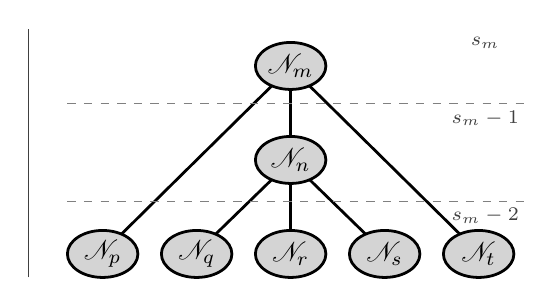
\begin{tikzpicture}[>=latex,line join=bevel,scale=0.47]
  \pgfsetlinewidth{1bp}
%%
\begin{scope}
  \pgfsetstrokecolor{black}
  \definecolor{strokecol}{rgb}{1.0,1.0,1.0};
  \pgfsetstrokecolor{strokecol}
  \definecolor{fillcol}{rgb}{1.0,1.0,1.0};
  \pgfsetfillcolor{fillcol}
  \filldraw (0bp,0bp) -- (0bp,180bp) -- (342bp,180bp) -- (342bp,0bp) -- cycle;
\end{scope}
  \pgfsetcolor{black}
  % Edge: c2 -> c6
  \draw [-] (156.43bp,74.834bp) .. controls (146.25bp,64.938bp) and (132.48bp,51.546bp)  .. (113.8bp,33.385bp);
  % Edge: root -> c4
  \draw [-] (156.4bp,146.6bp) .. controls (131.06bp,121.62bp) and (78.82bp,70.101bp)  .. (41.639bp,33.435bp);
  % Edge: c2 -> c8
  \draw [-] (185.57bp,74.834bp) .. controls (195.75bp,64.938bp) and (209.52bp,51.546bp)  .. (228.2bp,33.385bp);
  % Edge: root -> c10
  \draw [-] (185.6bp,146.6bp) .. controls (210.94bp,121.62bp) and (263.18bp,70.101bp)  .. (300.36bp,33.435bp);
  % Edge: root -> c2
  \draw [-] (171bp,143.7bp) .. controls (171bp,135.98bp) and (171bp,126.71bp)  .. (171bp,108.1bp);
  % Edge: c2 -> c7
  \draw [-] (171bp,71.697bp) .. controls (171bp,63.983bp) and (171bp,54.712bp)  .. (171bp,36.104bp);
  % Node: c7
\begin{scope}
  \definecolor{strokecol}{rgb}{0.0,0.0,0.0};
  \pgfsetstrokecolor{strokecol}
  \definecolor{fillcol}{rgb}{0.83,0.83,0.83};
  \pgfsetfillcolor{fillcol}
  \filldraw [opacity=1] (171bp,18bp) ellipse (27bp and 18bp);
  \draw (171bp,18bp) node {$\mathscr{N}_r$};
\end{scope}
  % Node: c8
\begin{scope}
  \definecolor{strokecol}{rgb}{0.0,0.0,0.0};
  \pgfsetstrokecolor{strokecol}
  \definecolor{fillcol}{rgb}{0.83,0.83,0.83};
  \pgfsetfillcolor{fillcol}
  \filldraw [opacity=1] (243bp,18bp) ellipse (27bp and 18bp);
  \draw (243bp,18bp) node {$\mathscr{N}_s$};
\end{scope}
  % Node: c2
\begin{scope}
  \definecolor{strokecol}{rgb}{0.0,0.0,0.0};
  \pgfsetstrokecolor{strokecol}
  \definecolor{fillcol}{rgb}{0.83,0.83,0.83};
  \pgfsetfillcolor{fillcol}
  \filldraw [opacity=1] (171bp,90bp) ellipse (27bp and 18bp);
  \draw (171bp,90bp) node {$\mathscr{N}_n$};
\end{scope}
  % Node: c10
\begin{scope}
  \definecolor{strokecol}{rgb}{0.0,0.0,0.0};
  \pgfsetstrokecolor{strokecol}
  \definecolor{fillcol}{rgb}{0.83,0.83,0.83};
  \pgfsetfillcolor{fillcol}
  \filldraw [opacity=1] (315bp,18bp) ellipse (27bp and 18bp);
  \draw (315bp,18bp) node {$\mathscr{N}_t$};
\end{scope}
  % Node: root
\begin{scope}
  \definecolor{strokecol}{rgb}{0.0,0.0,0.0};
  \pgfsetstrokecolor{strokecol}
  \definecolor{fillcol}{rgb}{0.83,0.83,0.83};
  \pgfsetfillcolor{fillcol}
  \filldraw [opacity=1] (171bp,162bp) ellipse (27bp and 18bp);
  \draw (171bp,162bp) node {$\mathscr{N}_m$};
\end{scope}
  % Node: c6
\begin{scope}
  \definecolor{strokecol}{rgb}{0.0,0.0,0.0};
  \pgfsetstrokecolor{strokecol}
  \definecolor{fillcol}{rgb}{0.83,0.83,0.83};
  \pgfsetfillcolor{fillcol}
  \filldraw [opacity=1] (99bp,18bp) ellipse (27bp and 18bp);
  \draw (99bp,18bp) node {$\mathscr{N}_q$};
\end{scope}
  % Node: c4
\begin{scope}
  \definecolor{strokecol}{rgb}{0.0,0.0,0.0};
  \pgfsetstrokecolor{strokecol}
  \definecolor{fillcol}{rgb}{0.83,0.83,0.83};
  \pgfsetfillcolor{fillcol}
  \filldraw [opacity=1] (27bp,18bp) ellipse (27bp and 18bp);
  \draw (27bp,18bp) node {$\mathscr{N}_p$};
\end{scope}
%
\draw[darkgray, thin] (-30bp,0bp) -- (-30bp,190bp);
\draw[gray,thin,dashed] (0bp,58bp) -- (350bp,58bp);
\draw[gray,thin,dashed] (0bp,133bp) -- (350bp,133bp);

\draw (320bp,180bp) node[darkgray] {\scriptsize $s_m$};
\draw (320bp,122bp) node[darkgray] {\scriptsize $s_m - 1$};
\draw (320bp,47bp) node[darkgray] {\scriptsize $s_m - 2$};
\end{tikzpicture}


  \end{center}
  \caption{Imbalanced cover tree.}
  \label{fig:imbalance-bad}
\end{subfigure}
\caption{Balanced and imbalanced cover trees.}
\label{fig:imbalance}
\end{figure}

An imbalanced cover tree can---and often does---happen in practice, and the
imbalance may be far worse than the simple graphs of Figure \ref{fig:imbalance}.
Consider a dataset with a single outlier which is very far away from all of the
other points\footnote{Note also that for an outlier sufficiently far away, the
expansion constant is $N - 1$.}.  Figure \ref{fig:outlier} shows what happens in
this situation: the root node has two children; one of these children has only
the outlier as a descendant, and the other child has the rest of the points in
the dataset as a descendant.  In fact, it is easy to find datasets with multiple
outliers which give rise to a chain-like structure at the top of the tree: see
Figure \ref{fig:outliers} for an illustration\footnote{As a side note, this
behavior is not limited to cover trees, and can happen to mean-split $kd$-trees
too, especially in higher dimensions.}.

\begin{figure}
\begin{center}
  
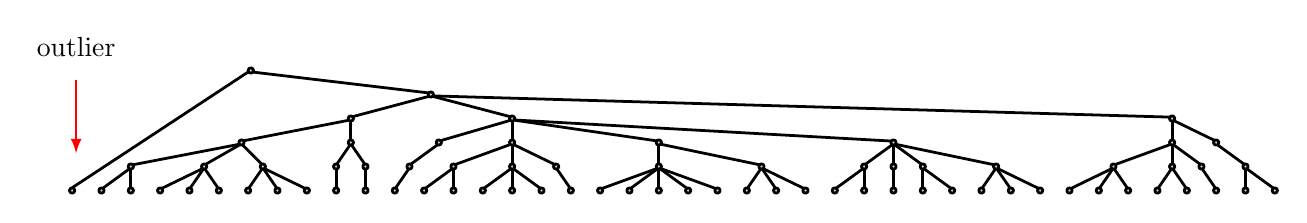
\begin{tikzpicture}[>=latex,line join=bevel,scale=0.48]
  \pgfsetlinewidth{1bp}
%%
\begin{scope}
  \pgfsetstrokecolor{black}
  \definecolor{strokecol}{rgb}{1.0,1.0,1.0};
  \pgfsetstrokecolor{strokecol}
  \definecolor{fillcol}{rgb}{1.0,1.0,1.0};
  \pgfsetfillcolor{fillcol}
  \filldraw (0bp,0bp) -- (0bp,94bp) -- (906bp,94bp) -- (906bp,0bp) -- cycle;
\end{scope}
\begin{scope}
  \pgfsetstrokecolor{black}
  \definecolor{strokecol}{rgb}{1.0,1.0,1.0};
  \pgfsetstrokecolor{strokecol}
  \definecolor{fillcol}{rgb}{1.0,1.0,1.0};
  \pgfsetfillcolor{fillcol}
  \filldraw (0bp,0bp) -- (0bp,94bp) -- (906bp,94bp) -- (906bp,0bp) -- cycle;
\end{scope}
\begin{scope}
  \pgfsetstrokecolor{black}
  \definecolor{strokecol}{rgb}{1.0,1.0,1.0};
  \pgfsetstrokecolor{strokecol}
  \definecolor{fillcol}{rgb}{1.0,1.0,1.0};
  \pgfsetfillcolor{fillcol}
  \filldraw (0bp,0bp) -- (0bp,94bp) -- (906bp,94bp) -- (906bp,0bp) -- cycle;
\end{scope}
\begin{scope}
  \pgfsetstrokecolor{black}
  \definecolor{strokecol}{rgb}{1.0,1.0,1.0};
  \pgfsetstrokecolor{strokecol}
  \definecolor{fillcol}{rgb}{1.0,1.0,1.0};
  \pgfsetfillcolor{fillcol}
  \filldraw (0bp,0bp) -- (0bp,94bp) -- (906bp,94bp) -- (906bp,0bp) -- cycle;
\end{scope}
\begin{scope}
  \pgfsetstrokecolor{black}
  \definecolor{strokecol}{rgb}{1.0,1.0,1.0};
  \pgfsetstrokecolor{strokecol}
  \definecolor{fillcol}{rgb}{1.0,1.0,1.0};
  \pgfsetfillcolor{fillcol}
  \filldraw (0bp,0bp) -- (0bp,94bp) -- (906bp,94bp) -- (906bp,0bp) -- cycle;
\end{scope}
\begin{scope}
  \pgfsetstrokecolor{black}
  \definecolor{strokecol}{rgb}{1.0,1.0,1.0};
  \pgfsetstrokecolor{strokecol}
  \definecolor{fillcol}{rgb}{1.0,1.0,1.0};
  \pgfsetfillcolor{fillcol}
  \filldraw (0bp,0bp) -- (0bp,94bp) -- (906bp,94bp) -- (906bp,0bp) -- cycle;
\end{scope}
\begin{scope}
  \pgfsetstrokecolor{black}
  \definecolor{strokecol}{rgb}{1.0,1.0,1.0};
  \pgfsetstrokecolor{strokecol}
  \definecolor{fillcol}{rgb}{1.0,1.0,1.0};
  \pgfsetfillcolor{fillcol}
  \filldraw (0bp,0bp) -- (0bp,94bp) -- (906bp,94bp) -- (906bp,0bp) -- cycle;
\end{scope}
\begin{scope}
  \pgfsetstrokecolor{black}
  \definecolor{strokecol}{rgb}{1.0,1.0,1.0};
  \pgfsetstrokecolor{strokecol}
  \definecolor{fillcol}{rgb}{1.0,1.0,1.0};
  \pgfsetfillcolor{fillcol}
  \filldraw (0bp,0bp) -- (0bp,94bp) -- (906bp,94bp) -- (906bp,0bp) -- cycle;
\end{scope}
\begin{scope}
  \pgfsetstrokecolor{black}
  \definecolor{strokecol}{rgb}{1.0,1.0,1.0};
  \pgfsetstrokecolor{strokecol}
  \definecolor{fillcol}{rgb}{1.0,1.0,1.0};
  \pgfsetfillcolor{fillcol}
  \filldraw (0bp,0bp) -- (0bp,94bp) -- (906bp,94bp) -- (906bp,0bp) -- cycle;
\end{scope}
\begin{scope}
  \pgfsetstrokecolor{black}
  \definecolor{strokecol}{rgb}{1.0,1.0,1.0};
  \pgfsetstrokecolor{strokecol}
  \definecolor{fillcol}{rgb}{1.0,1.0,1.0};
  \pgfsetfillcolor{fillcol}
  \filldraw (0bp,0bp) -- (0bp,94bp) -- (906bp,94bp) -- (906bp,0bp) -- cycle;
\end{scope}
\begin{scope}
  \pgfsetstrokecolor{black}
  \definecolor{strokecol}{rgb}{1.0,1.0,1.0};
  \pgfsetstrokecolor{strokecol}
  \definecolor{fillcol}{rgb}{1.0,1.0,1.0};
  \pgfsetfillcolor{fillcol}
  \filldraw (0bp,0bp) -- (0bp,94bp) -- (906bp,94bp) -- (906bp,0bp) -- cycle;
\end{scope}
\begin{scope}
  \pgfsetstrokecolor{black}
  \definecolor{strokecol}{rgb}{1.0,1.0,1.0};
  \pgfsetstrokecolor{strokecol}
  \definecolor{fillcol}{rgb}{1.0,1.0,1.0};
  \pgfsetfillcolor{fillcol}
  \filldraw (0bp,0bp) -- (0bp,94bp) -- (906bp,94bp) -- (906bp,0bp) -- cycle;
\end{scope}
\begin{scope}
  \pgfsetstrokecolor{black}
  \definecolor{strokecol}{rgb}{1.0,1.0,1.0};
  \pgfsetstrokecolor{strokecol}
  \definecolor{fillcol}{rgb}{1.0,1.0,1.0};
  \pgfsetfillcolor{fillcol}
  \filldraw (0bp,0bp) -- (0bp,94bp) -- (906bp,94bp) -- (906bp,0bp) -- cycle;
\end{scope}
\begin{scope}
  \pgfsetstrokecolor{black}
  \definecolor{strokecol}{rgb}{1.0,1.0,1.0};
  \pgfsetstrokecolor{strokecol}
  \definecolor{fillcol}{rgb}{1.0,1.0,1.0};
  \pgfsetfillcolor{fillcol}
  \filldraw (0bp,0bp) -- (0bp,94bp) -- (906bp,94bp) -- (906bp,0bp) -- cycle;
\end{scope}
\begin{scope}
  \pgfsetstrokecolor{black}
  \definecolor{strokecol}{rgb}{1.0,1.0,1.0};
  \pgfsetstrokecolor{strokecol}
  \definecolor{fillcol}{rgb}{1.0,1.0,1.0};
  \pgfsetfillcolor{fillcol}
  \filldraw (0bp,0bp) -- (0bp,94bp) -- (906bp,94bp) -- (906bp,0bp) -- cycle;
\end{scope}
\begin{scope}
  \pgfsetstrokecolor{black}
  \definecolor{strokecol}{rgb}{1.0,1.0,1.0};
  \pgfsetstrokecolor{strokecol}
  \definecolor{fillcol}{rgb}{1.0,1.0,1.0};
  \pgfsetfillcolor{fillcol}
  \filldraw (0bp,0bp) -- (0bp,94bp) -- (906bp,94bp) -- (906bp,0bp) -- cycle;
\end{scope}
\begin{scope}
  \pgfsetstrokecolor{black}
  \definecolor{strokecol}{rgb}{1.0,1.0,1.0};
  \pgfsetstrokecolor{strokecol}
  \definecolor{fillcol}{rgb}{1.0,1.0,1.0};
  \pgfsetfillcolor{fillcol}
  \filldraw (0bp,0bp) -- (0bp,94bp) -- (906bp,94bp) -- (906bp,0bp) -- cycle;
\end{scope}
\begin{scope}
  \pgfsetstrokecolor{black}
  \definecolor{strokecol}{rgb}{1.0,1.0,1.0};
  \pgfsetstrokecolor{strokecol}
  \definecolor{fillcol}{rgb}{1.0,1.0,1.0};
  \pgfsetfillcolor{fillcol}
  \filldraw (0bp,0bp) -- (0bp,94bp) -- (906bp,94bp) -- (906bp,0bp) -- cycle;
\end{scope}
\begin{scope}
  \pgfsetstrokecolor{black}
  \definecolor{strokecol}{rgb}{1.0,1.0,1.0};
  \pgfsetstrokecolor{strokecol}
  \definecolor{fillcol}{rgb}{1.0,1.0,1.0};
  \pgfsetfillcolor{fillcol}
  \filldraw (0bp,0bp) -- (0bp,94bp) -- (906bp,94bp) -- (906bp,0bp) -- cycle;
\end{scope}
\begin{scope}
  \pgfsetstrokecolor{black}
  \definecolor{strokecol}{rgb}{1.0,1.0,1.0};
  \pgfsetstrokecolor{strokecol}
  \definecolor{fillcol}{rgb}{1.0,1.0,1.0};
  \pgfsetfillcolor{fillcol}
  \filldraw (0bp,0bp) -- (0bp,94bp) -- (906bp,94bp) -- (906bp,0bp) -- cycle;
\end{scope}
\begin{scope}
  \pgfsetstrokecolor{black}
  \definecolor{strokecol}{rgb}{1.0,1.0,1.0};
  \pgfsetstrokecolor{strokecol}
  \definecolor{fillcol}{rgb}{1.0,1.0,1.0};
  \pgfsetfillcolor{fillcol}
  \filldraw (0bp,0bp) -- (0bp,94bp) -- (906bp,94bp) -- (906bp,0bp) -- cycle;
\end{scope}
\begin{scope}
  \pgfsetstrokecolor{black}
  \definecolor{strokecol}{rgb}{1.0,1.0,1.0};
  \pgfsetstrokecolor{strokecol}
  \definecolor{fillcol}{rgb}{1.0,1.0,1.0};
  \pgfsetfillcolor{fillcol}
  \filldraw (0bp,0bp) -- (0bp,94bp) -- (906bp,94bp) -- (906bp,0bp) -- cycle;
\end{scope}
\begin{scope}
  \pgfsetstrokecolor{black}
  \definecolor{strokecol}{rgb}{1.0,1.0,1.0};
  \pgfsetstrokecolor{strokecol}
  \definecolor{fillcol}{rgb}{1.0,1.0,1.0};
  \pgfsetfillcolor{fillcol}
  \filldraw (0bp,0bp) -- (0bp,94bp) -- (906bp,94bp) -- (906bp,0bp) -- cycle;
\end{scope}
\begin{scope}
  \pgfsetstrokecolor{black}
  \definecolor{strokecol}{rgb}{1.0,1.0,1.0};
  \pgfsetstrokecolor{strokecol}
  \definecolor{fillcol}{rgb}{1.0,1.0,1.0};
  \pgfsetfillcolor{fillcol}
  \filldraw (0bp,0bp) -- (0bp,94bp) -- (906bp,94bp) -- (906bp,0bp) -- cycle;
\end{scope}
\begin{scope}
  \pgfsetstrokecolor{black}
  \definecolor{strokecol}{rgb}{1.0,1.0,1.0};
  \pgfsetstrokecolor{strokecol}
  \definecolor{fillcol}{rgb}{1.0,1.0,1.0};
  \pgfsetfillcolor{fillcol}
  \filldraw (0bp,0bp) -- (0bp,94bp) -- (906bp,94bp) -- (906bp,0bp) -- cycle;
\end{scope}
\begin{scope}
  \pgfsetstrokecolor{black}
  \definecolor{strokecol}{rgb}{1.0,1.0,1.0};
  \pgfsetstrokecolor{strokecol}
  \definecolor{fillcol}{rgb}{1.0,1.0,1.0};
  \pgfsetfillcolor{fillcol}
  \filldraw (0bp,0bp) -- (0bp,94bp) -- (906bp,94bp) -- (906bp,0bp) -- cycle;
\end{scope}
\begin{scope}
  \pgfsetstrokecolor{black}
  \definecolor{strokecol}{rgb}{1.0,1.0,1.0};
  \pgfsetstrokecolor{strokecol}
  \definecolor{fillcol}{rgb}{1.0,1.0,1.0};
  \pgfsetfillcolor{fillcol}
  \filldraw (0bp,0bp) -- (0bp,94bp) -- (906bp,94bp) -- (906bp,0bp) -- cycle;
\end{scope}
\begin{scope}
  \pgfsetstrokecolor{black}
  \definecolor{strokecol}{rgb}{1.0,1.0,1.0};
  \pgfsetstrokecolor{strokecol}
  \definecolor{fillcol}{rgb}{1.0,1.0,1.0};
  \pgfsetfillcolor{fillcol}
  \filldraw (0bp,0bp) -- (0bp,94bp) -- (906bp,94bp) -- (906bp,0bp) -- cycle;
\end{scope}
  \pgfsetcolor{black}
  % Edge: c12 -> c30
  \draw [-] (827bp,35.95bp) -- (827bp,22.075bp);
  % Edge: c8 -> c19
  \draw [-] (275.82bp,36.14bp) -- (256.08bp,21.788bp);
  % Edge: c23 -> c54
  \draw [-] (443.46bp,18.468bp) -- (484.49bp,3.5508bp);
  % Edge: c28 -> c65
  \draw [-] (696.42bp,18.312bp) -- (726.62bp,3.6671bp);
  % Edge: c6 -> c16
  \draw [-] (130.05bp,35.95bp) -- (143.93bp,22.075bp);
  % Edge: c18 -> c42
  \draw [-] (222bp,17.95bp) -- (222bp,4.0746bp);
  % Edge: c2 -> c4
  \draw [-] (272.51bp,72.604bp) -- (330.32bp,57.44bp);
  % Edge: c27 -> c61
  \draw [-] (640bp,17.95bp) -- (640bp,4.0746bp);
  % Edge: c4 -> c8
  \draw [-] (330.17bp,54.468bp) -- (278.46bp,39.426bp);
  % Edge: c7 -> c17
  \draw [-] (210.28bp,35.95bp) -- (200.74bp,22.075bp);
  % Edge: c16 -> c38
  \draw [-] (144.28bp,17.95bp) -- (134.74bp,4.0746bp);
  % Edge: c10 -> c24
  \draw [-] (443.61bp,36.666bp) -- (517.4bp,21.332bp);
  % Edge: c23 -> c50
  \draw [-] (440.54bp,18.468bp) -- (399.51bp,3.5508bp);
  % Edge: c4 -> c10
  \draw [-] (333.91bp,54.722bp) -- (440.37bp,39.237bp);
  % Edge: c29 -> c67
  \draw [-] (782.28bp,17.95bp) -- (772.74bp,4.0746bp);
  % Edge: c12 -> c29
  \draw [-] (825.54bp,36.468bp) -- (784.51bp,21.551bp);
  % Edge: c23 -> c51
  \draw [-] (440.82bp,18.14bp) -- (421.08bp,3.788bp);
  % Edge: c16 -> c40
  \draw [-] (146.42bp,18.312bp) -- (176.62bp,3.6671bp);
  % Edge: root -> c2
  \draw [-] (137.91bp,90.774bp) -- (269.34bp,75.196bp);
  % Edge: c12 -> c31
  \draw [-] (828.18bp,36.14bp) -- (847.92bp,21.788bp);
  % Edge: c17 -> c41
  \draw [-] (200bp,17.95bp) -- (200bp,4.0746bp);
  % Edge: c2 -> c5
  \draw [-] (273.01bp,72.942bp) -- (825.12bp,57.054bp);
  % Edge: c23 -> c52
  \draw [-] (442bp,17.95bp) -- (442bp,4.0746bp);
  % Edge: c4 -> c9
  \draw [-] (332bp,53.95bp) -- (332bp,40.075bp);
  % Edge: c9 -> c20
  \draw [-] (330.54bp,36.468bp) -- (289.51bp,21.551bp);
  % Edge: c27 -> c62
  \draw [-] (641.18bp,18.14bp) -- (660.92bp,3.788bp);
  % Edge: c16 -> c39
  \draw [-] (145.72bp,17.95bp) -- (155.26bp,4.0746bp);
  % Edge: c22 -> c49
  \draw [-] (365.72bp,17.95bp) -- (375.26bp,4.0746bp);
  % Edge: c4 -> c11
  \draw [-] (333.83bp,54.898bp) -- (616.05bp,39.109bp);
  % Edge: c23 -> c53
  \draw [-] (443.18bp,18.14bp) -- (462.92bp,3.788bp);
  % Edge: c20 -> c44
  \draw [-] (286.82bp,18.14bp) -- (267.08bp,3.788bp);
  % Edge: c32 -> c73
  \draw [-] (883.18bp,18.14bp) -- (902.92bp,3.788bp);
  % Edge: c11 -> c25
  \draw [-] (616.82bp,36.14bp) -- (597.08bp,21.788bp);
  % Edge: root -> c1
  \draw [-] (134.11bp,90.943bp) -- (2bp,4.0576bp);
  % Edge: c15 -> c37
  \draw [-] (101.72bp,17.95bp) -- (111.26bp,4.0746bp);
  % Edge: c21 -> c46
  \draw [-] (330.82bp,18.14bp) -- (311.08bp,3.788bp);
  % Edge: c7 -> c18
  \draw [-] (211.72bp,35.95bp) -- (221.26bp,22.075bp);
  % Edge: c25 -> c59
  \draw [-] (596bp,17.95bp) -- (596bp,4.0746bp);
  % Edge: c10 -> c23
  \draw [-] (442bp,35.95bp) -- (442bp,22.075bp);
  % Edge: c9 -> c21
  \draw [-] (332bp,35.95bp) -- (332bp,22.075bp);
  % Edge: c3 -> c7
  \draw [-] (211bp,53.95bp) -- (211bp,40.075bp);
  % Edge: c30 -> c70
  \draw [-] (827.72bp,17.95bp) -- (837.26bp,4.0746bp);
  % Edge: c28 -> c63
  \draw [-] (694.28bp,17.95bp) -- (684.74bp,4.0746bp);
  % Edge: c6 -> c14
  \draw [-] (127.27bp,36.666bp) -- (47.724bp,21.332bp);
  % Edge: c24 -> c57
  \draw [-] (520.42bp,18.312bp) -- (550.62bp,3.6671bp);
  % Edge: c20 -> c45
  \draw [-] (288bp,17.95bp) -- (288bp,4.0746bp);
  % Edge: c26 -> c60
  \draw [-] (618bp,17.95bp) -- (618bp,4.0746bp);
  % Edge: c14 -> c34
  \draw [-] (46bp,17.95bp) -- (46bp,4.0746bp);
  % Edge: c11 -> c26
  \draw [-] (618bp,35.95bp) -- (618bp,22.075bp);
  % Edge: c21 -> c48
  \draw [-] (333.18bp,18.14bp) -- (352.92bp,3.788bp);
  % Edge: c14 -> c33
  \draw [-] (44.817bp,18.14bp) -- (25.083bp,3.788bp);
  % Edge: c31 -> c71
  \draw [-] (849.72bp,17.95bp) -- (859.26bp,4.0746bp);
  % Edge: c5 -> c13
  \draw [-] (828.42bp,54.312bp) -- (858.62bp,39.667bp);
  % Edge: c13 -> c32
  \draw [-] (861.18bp,36.14bp) -- (880.92bp,21.788bp);
  % Edge: c25 -> c58
  \draw [-] (594.82bp,18.14bp) -- (575.08bp,3.788bp);
  % Edge: c15 -> c36
  \draw [-] (100.28bp,17.95bp) -- (90.739bp,4.0746bp);
  % Edge: c9 -> c22
  \draw [-] (333.42bp,36.312bp) -- (363.62bp,21.667bp);
  % Edge: c3 -> c6
  \draw [-] (209.29bp,54.666bp) -- (130.7bp,39.332bp);
  % Edge: c21 -> c47
  \draw [-] (332bp,17.95bp) -- (332bp,4.0746bp);
  % Edge: c30 -> c69
  \draw [-] (826.28bp,17.95bp) -- (816.74bp,4.0746bp);
  % Edge: c28 -> c64
  \draw [-] (695.72bp,17.95bp) -- (705.26bp,4.0746bp);
  % Edge: c6 -> c15
  \draw [-] (127.8bp,36.312bp) -- (102.17bp,21.667bp);
  % Edge: c2 -> c3
  \draw [-] (269.52bp,72.604bp) -- (212.65bp,57.44bp);
  % Edge: c19 -> c43
  \draw [-] (254.28bp,17.95bp) -- (244.74bp,4.0746bp);
  % Edge: c29 -> c66
  \draw [-] (781.58bp,18.312bp) -- (751.38bp,3.6671bp);
  % Edge: c11 -> c27
  \draw [-] (619.18bp,36.14bp) -- (638.92bp,21.788bp);
  % Edge: c24 -> c55
  \draw [-] (518.28bp,17.95bp) -- (508.74bp,4.0746bp);
  % Edge: c24 -> c56
  \draw [-] (519.72bp,17.95bp) -- (529.26bp,4.0746bp);
  % Edge: c11 -> c28
  \draw [-] (619.61bp,36.666bp) -- (693.4bp,21.332bp);
  % Edge: c32 -> c72
  \draw [-] (882bp,17.95bp) -- (882bp,4.0746bp);
  % Edge: c5 -> c12
  \draw [-] (827bp,53.95bp) -- (827bp,40.075bp);
  % Edge: c15 -> c35
  \draw [-] (99.582bp,18.312bp) -- (69.376bp,3.6671bp);
  % Edge: c29 -> c68
  \draw [-] (783.72bp,17.95bp) -- (793.26bp,4.0746bp);
  % Node: c10
\begin{scope}
  \definecolor{strokecol}{rgb}{0.0,0.0,0.0};
  \pgfsetstrokecolor{strokecol}
  \definecolor{fillcol}{rgb}{0.83,0.83,0.83};
  \pgfsetfillcolor{fillcol}
  \filldraw [opacity=1] (442bp,38bp) ellipse (2bp and 2bp);
\end{scope}
  % Node: c65
\begin{scope}
  \definecolor{strokecol}{rgb}{0.0,0.0,0.0};
  \pgfsetstrokecolor{strokecol}
  \definecolor{fillcol}{rgb}{0.83,0.83,0.83};
  \pgfsetfillcolor{fillcol}
  \filldraw [opacity=1] (728bp,2bp) ellipse (2bp and 2bp);
\end{scope}
  % Node: c69
\begin{scope}
  \definecolor{strokecol}{rgb}{0.0,0.0,0.0};
  \pgfsetstrokecolor{strokecol}
  \definecolor{fillcol}{rgb}{0.83,0.83,0.83};
  \pgfsetfillcolor{fillcol}
  \filldraw [opacity=1] (816bp,2bp) ellipse (2bp and 2bp);
\end{scope}
  % Node: c62
\begin{scope}
  \definecolor{strokecol}{rgb}{0.0,0.0,0.0};
  \pgfsetstrokecolor{strokecol}
  \definecolor{fillcol}{rgb}{0.83,0.83,0.83};
  \pgfsetfillcolor{fillcol}
  \filldraw [opacity=1] (662bp,2bp) ellipse (2bp and 2bp);
\end{scope}
  % Node: c63
\begin{scope}
  \definecolor{strokecol}{rgb}{0.0,0.0,0.0};
  \pgfsetstrokecolor{strokecol}
  \definecolor{fillcol}{rgb}{0.83,0.83,0.83};
  \pgfsetfillcolor{fillcol}
  \filldraw [opacity=1] (684bp,2bp) ellipse (2bp and 2bp);
\end{scope}
  % Node: c4
\begin{scope}
  \definecolor{strokecol}{rgb}{0.0,0.0,0.0};
  \pgfsetstrokecolor{strokecol}
  \definecolor{fillcol}{rgb}{0.83,0.83,0.83};
  \pgfsetfillcolor{fillcol}
  \filldraw [opacity=1] (332bp,56bp) ellipse (2bp and 2bp);
\end{scope}
  % Node: c2
\begin{scope}
  \definecolor{strokecol}{rgb}{0.0,0.0,0.0};
  \pgfsetstrokecolor{strokecol}
  \definecolor{fillcol}{rgb}{0.83,0.83,0.83};
  \pgfsetfillcolor{fillcol}
  \filldraw [opacity=1] (271bp,74bp) ellipse (2bp and 2bp);
\end{scope}
  % Node: c61
\begin{scope}
  \definecolor{strokecol}{rgb}{0.0,0.0,0.0};
  \pgfsetstrokecolor{strokecol}
  \definecolor{fillcol}{rgb}{0.83,0.83,0.83};
  \pgfsetfillcolor{fillcol}
  \filldraw [opacity=1] (640bp,2bp) ellipse (2bp and 2bp);
\end{scope}
  % Node: c57
\begin{scope}
  \definecolor{strokecol}{rgb}{0.0,0.0,0.0};
  \pgfsetstrokecolor{strokecol}
  \definecolor{fillcol}{rgb}{0.83,0.83,0.83};
  \pgfsetfillcolor{fillcol}
  \filldraw [opacity=1] (552bp,2bp) ellipse (2bp and 2bp);
\end{scope}
  % Node: c56
\begin{scope}
  \definecolor{strokecol}{rgb}{0.0,0.0,0.0};
  \pgfsetstrokecolor{strokecol}
  \definecolor{fillcol}{rgb}{0.83,0.83,0.83};
  \pgfsetfillcolor{fillcol}
  \filldraw [opacity=1] (530bp,2bp) ellipse (2bp and 2bp);
\end{scope}
  % Node: c55
\begin{scope}
  \definecolor{strokecol}{rgb}{0.0,0.0,0.0};
  \pgfsetstrokecolor{strokecol}
  \definecolor{fillcol}{rgb}{0.83,0.83,0.83};
  \pgfsetfillcolor{fillcol}
  \filldraw [opacity=1] (508bp,2bp) ellipse (2bp and 2bp);
\end{scope}
  % Node: c54
\begin{scope}
  \definecolor{strokecol}{rgb}{0.0,0.0,0.0};
  \pgfsetstrokecolor{strokecol}
  \definecolor{fillcol}{rgb}{0.83,0.83,0.83};
  \pgfsetfillcolor{fillcol}
  \filldraw [opacity=1] (486bp,2bp) ellipse (2bp and 2bp);
\end{scope}
  % Node: c53
\begin{scope}
  \definecolor{strokecol}{rgb}{0.0,0.0,0.0};
  \pgfsetstrokecolor{strokecol}
  \definecolor{fillcol}{rgb}{0.83,0.83,0.83};
  \pgfsetfillcolor{fillcol}
  \filldraw [opacity=1] (464bp,2bp) ellipse (2bp and 2bp);
\end{scope}
  % Node: c52
\begin{scope}
  \definecolor{strokecol}{rgb}{0.0,0.0,0.0};
  \pgfsetstrokecolor{strokecol}
  \definecolor{fillcol}{rgb}{0.83,0.83,0.83};
  \pgfsetfillcolor{fillcol}
  \filldraw [opacity=1] (442bp,2bp) ellipse (2bp and 2bp);
\end{scope}
  % Node: c51
\begin{scope}
  \definecolor{strokecol}{rgb}{0.0,0.0,0.0};
  \pgfsetstrokecolor{strokecol}
  \definecolor{fillcol}{rgb}{0.83,0.83,0.83};
  \pgfsetfillcolor{fillcol}
  \filldraw [opacity=1] (420bp,2bp) ellipse (2bp and 2bp);
\end{scope}
  % Node: c50
\begin{scope}
  \definecolor{strokecol}{rgb}{0.0,0.0,0.0};
  \pgfsetstrokecolor{strokecol}
  \definecolor{fillcol}{rgb}{0.83,0.83,0.83};
  \pgfsetfillcolor{fillcol}
  \filldraw [opacity=1] (398bp,2bp) ellipse (2bp and 2bp);
\end{scope}
  % Node: c71
\begin{scope}
  \definecolor{strokecol}{rgb}{0.0,0.0,0.0};
  \pgfsetstrokecolor{strokecol}
  \definecolor{fillcol}{rgb}{0.83,0.83,0.83};
  \pgfsetfillcolor{fillcol}
  \filldraw [opacity=1] (860bp,2bp) ellipse (2bp and 2bp);
\end{scope}
  % Node: c70
\begin{scope}
  \definecolor{strokecol}{rgb}{0.0,0.0,0.0};
  \pgfsetstrokecolor{strokecol}
  \definecolor{fillcol}{rgb}{0.83,0.83,0.83};
  \pgfsetfillcolor{fillcol}
  \filldraw [opacity=1] (838bp,2bp) ellipse (2bp and 2bp);
\end{scope}
  % Node: c73
\begin{scope}
  \definecolor{strokecol}{rgb}{0.0,0.0,0.0};
  \pgfsetstrokecolor{strokecol}
  \definecolor{fillcol}{rgb}{0.83,0.83,0.83};
  \pgfsetfillcolor{fillcol}
  \filldraw [opacity=1] (904bp,2bp) ellipse (2bp and 2bp);
\end{scope}
  % Node: c72
\begin{scope}
  \definecolor{strokecol}{rgb}{0.0,0.0,0.0};
  \pgfsetstrokecolor{strokecol}
  \definecolor{fillcol}{rgb}{0.83,0.83,0.83};
  \pgfsetfillcolor{fillcol}
  \filldraw [opacity=1] (882bp,2bp) ellipse (2bp and 2bp);
\end{scope}
  % Node: c59
\begin{scope}
  \definecolor{strokecol}{rgb}{0.0,0.0,0.0};
  \pgfsetstrokecolor{strokecol}
  \definecolor{fillcol}{rgb}{0.83,0.83,0.83};
  \pgfsetfillcolor{fillcol}
  \filldraw [opacity=1] (596bp,2bp) ellipse (2bp and 2bp);
\end{scope}
  % Node: c58
\begin{scope}
  \definecolor{strokecol}{rgb}{0.0,0.0,0.0};
  \pgfsetstrokecolor{strokecol}
  \definecolor{fillcol}{rgb}{0.83,0.83,0.83};
  \pgfsetfillcolor{fillcol}
  \filldraw [opacity=1] (574bp,2bp) ellipse (2bp and 2bp);
\end{scope}
  % Node: c19
\begin{scope}
  \definecolor{strokecol}{rgb}{0.0,0.0,0.0};
  \pgfsetstrokecolor{strokecol}
  \definecolor{fillcol}{rgb}{0.83,0.83,0.83};
  \pgfsetfillcolor{fillcol}
  \filldraw [opacity=1] (255bp,20bp) ellipse (2bp and 2bp);
\end{scope}
  % Node: c18
\begin{scope}
  \definecolor{strokecol}{rgb}{0.0,0.0,0.0};
  \pgfsetstrokecolor{strokecol}
  \definecolor{fillcol}{rgb}{0.83,0.83,0.83};
  \pgfsetfillcolor{fillcol}
  \filldraw [opacity=1] (222bp,20bp) ellipse (2bp and 2bp);
\end{scope}
  % Node: c39
\begin{scope}
  \definecolor{strokecol}{rgb}{0.0,0.0,0.0};
  \pgfsetstrokecolor{strokecol}
  \definecolor{fillcol}{rgb}{0.83,0.83,0.83};
  \pgfsetfillcolor{fillcol}
  \filldraw [opacity=1] (156bp,2bp) ellipse (2bp and 2bp);
\end{scope}
  % Node: c38
\begin{scope}
  \definecolor{strokecol}{rgb}{0.0,0.0,0.0};
  \pgfsetstrokecolor{strokecol}
  \definecolor{fillcol}{rgb}{0.83,0.83,0.83};
  \pgfsetfillcolor{fillcol}
  \filldraw [opacity=1] (134bp,2bp) ellipse (2bp and 2bp);
\end{scope}
  % Node: c35
\begin{scope}
  \definecolor{strokecol}{rgb}{0.0,0.0,0.0};
  \pgfsetstrokecolor{strokecol}
  \definecolor{fillcol}{rgb}{0.83,0.83,0.83};
  \pgfsetfillcolor{fillcol}
  \filldraw [opacity=1] (68bp,2bp) ellipse (2bp and 2bp);
\end{scope}
  % Node: c34
\begin{scope}
  \definecolor{strokecol}{rgb}{0.0,0.0,0.0};
  \pgfsetstrokecolor{strokecol}
  \definecolor{fillcol}{rgb}{0.83,0.83,0.83};
  \pgfsetfillcolor{fillcol}
  \filldraw [opacity=1] (46bp,2bp) ellipse (2bp and 2bp);
\end{scope}
  % Node: c37
\begin{scope}
  \definecolor{strokecol}{rgb}{0.0,0.0,0.0};
  \pgfsetstrokecolor{strokecol}
  \definecolor{fillcol}{rgb}{0.83,0.83,0.83};
  \pgfsetfillcolor{fillcol}
  \filldraw [opacity=1] (112bp,2bp) ellipse (2bp and 2bp);
\end{scope}
  % Node: c36
\begin{scope}
  \definecolor{strokecol}{rgb}{0.0,0.0,0.0};
  \pgfsetstrokecolor{strokecol}
  \definecolor{fillcol}{rgb}{0.83,0.83,0.83};
  \pgfsetfillcolor{fillcol}
  \filldraw [opacity=1] (90bp,2bp) ellipse (2bp and 2bp);
\end{scope}
  % Node: c31
\begin{scope}
  \definecolor{strokecol}{rgb}{0.0,0.0,0.0};
  \pgfsetstrokecolor{strokecol}
  \definecolor{fillcol}{rgb}{0.83,0.83,0.83};
  \pgfsetfillcolor{fillcol}
  \filldraw [opacity=1] (849bp,20bp) ellipse (2bp and 2bp);
\end{scope}
  % Node: c30
\begin{scope}
  \definecolor{strokecol}{rgb}{0.0,0.0,0.0};
  \pgfsetstrokecolor{strokecol}
  \definecolor{fillcol}{rgb}{0.83,0.83,0.83};
  \pgfsetfillcolor{fillcol}
  \filldraw [opacity=1] (827bp,20bp) ellipse (2bp and 2bp);
\end{scope}
  % Node: c33
\begin{scope}
  \definecolor{strokecol}{rgb}{0.0,0.0,0.0};
  \pgfsetstrokecolor{strokecol}
  \definecolor{fillcol}{rgb}{0.83,0.83,0.83};
  \pgfsetfillcolor{fillcol}
  \filldraw [opacity=1] (24bp,2bp) ellipse (2bp and 2bp);
\end{scope}
  % Node: c32
\begin{scope}
  \definecolor{strokecol}{rgb}{0.0,0.0,0.0};
  \pgfsetstrokecolor{strokecol}
  \definecolor{fillcol}{rgb}{0.83,0.83,0.83};
  \pgfsetfillcolor{fillcol}
  \filldraw [opacity=1] (882bp,20bp) ellipse (2bp and 2bp);
\end{scope}
  % Node: c44
\begin{scope}
  \definecolor{strokecol}{rgb}{0.0,0.0,0.0};
  \pgfsetstrokecolor{strokecol}
  \definecolor{fillcol}{rgb}{0.83,0.83,0.83};
  \pgfsetfillcolor{fillcol}
  \filldraw [opacity=1] (266bp,2bp) ellipse (2bp and 2bp);
\end{scope}
  % Node: c68
\begin{scope}
  \definecolor{strokecol}{rgb}{0.0,0.0,0.0};
  \pgfsetstrokecolor{strokecol}
  \definecolor{fillcol}{rgb}{0.83,0.83,0.83};
  \pgfsetfillcolor{fillcol}
  \filldraw [opacity=1] (794bp,2bp) ellipse (2bp and 2bp);
\end{scope}
  % Node: c11
\begin{scope}
  \definecolor{strokecol}{rgb}{0.0,0.0,0.0};
  \pgfsetstrokecolor{strokecol}
  \definecolor{fillcol}{rgb}{0.83,0.83,0.83};
  \pgfsetfillcolor{fillcol}
  \filldraw [opacity=1] (618bp,38bp) ellipse (2bp and 2bp);
\end{scope}
  % Node: c42
\begin{scope}
  \definecolor{strokecol}{rgb}{0.0,0.0,0.0};
  \pgfsetstrokecolor{strokecol}
  \definecolor{fillcol}{rgb}{0.83,0.83,0.83};
  \pgfsetfillcolor{fillcol}
  \filldraw [opacity=1] (222bp,2bp) ellipse (2bp and 2bp);
\end{scope}
  % Node: c45
\begin{scope}
  \definecolor{strokecol}{rgb}{0.0,0.0,0.0};
  \pgfsetstrokecolor{strokecol}
  \definecolor{fillcol}{rgb}{0.83,0.83,0.83};
  \pgfsetfillcolor{fillcol}
  \filldraw [opacity=1] (288bp,2bp) ellipse (2bp and 2bp);
\end{scope}
  % Node: c46
\begin{scope}
  \definecolor{strokecol}{rgb}{0.0,0.0,0.0};
  \pgfsetstrokecolor{strokecol}
  \definecolor{fillcol}{rgb}{0.83,0.83,0.83};
  \pgfsetfillcolor{fillcol}
  \filldraw [opacity=1] (310bp,2bp) ellipse (2bp and 2bp);
\end{scope}
  % Node: c13
\begin{scope}
  \definecolor{strokecol}{rgb}{0.0,0.0,0.0};
  \pgfsetstrokecolor{strokecol}
  \definecolor{fillcol}{rgb}{0.83,0.83,0.83};
  \pgfsetfillcolor{fillcol}
  \filldraw [opacity=1] (860bp,38bp) ellipse (2bp and 2bp);
\end{scope}
  % Node: c9
\begin{scope}
  \definecolor{strokecol}{rgb}{0.0,0.0,0.0};
  \pgfsetstrokecolor{strokecol}
  \definecolor{fillcol}{rgb}{0.83,0.83,0.83};
  \pgfsetfillcolor{fillcol}
  \filldraw [opacity=1] (332bp,38bp) ellipse (2bp and 2bp);
\end{scope}
  % Node: c47
\begin{scope}
  \definecolor{strokecol}{rgb}{0.0,0.0,0.0};
  \pgfsetstrokecolor{strokecol}
  \definecolor{fillcol}{rgb}{0.83,0.83,0.83};
  \pgfsetfillcolor{fillcol}
  \filldraw [opacity=1] (332bp,2bp) ellipse (2bp and 2bp);
\end{scope}
  % Node: c12
\begin{scope}
  \definecolor{strokecol}{rgb}{0.0,0.0,0.0};
  \pgfsetstrokecolor{strokecol}
  \definecolor{fillcol}{rgb}{0.83,0.83,0.83};
  \pgfsetfillcolor{fillcol}
  \filldraw [opacity=1] (827bp,38bp) ellipse (2bp and 2bp);
\end{scope}
  % Node: c3
\begin{scope}
  \definecolor{strokecol}{rgb}{0.0,0.0,0.0};
  \pgfsetstrokecolor{strokecol}
  \definecolor{fillcol}{rgb}{0.83,0.83,0.83};
  \pgfsetfillcolor{fillcol}
  \filldraw [opacity=1] (211bp,56bp) ellipse (2bp and 2bp);
\end{scope}
  % Node: c40
\begin{scope}
  \definecolor{strokecol}{rgb}{0.0,0.0,0.0};
  \pgfsetstrokecolor{strokecol}
  \definecolor{fillcol}{rgb}{0.83,0.83,0.83};
  \pgfsetfillcolor{fillcol}
  \filldraw [opacity=1] (178bp,2bp) ellipse (2bp and 2bp);
\end{scope}
  % Node: c1
\begin{scope}
  \definecolor{strokecol}{rgb}{0.0,0.0,0.0};
  \pgfsetstrokecolor{strokecol}
  \definecolor{fillcol}{rgb}{0.83,0.83,0.83};
  \pgfsetfillcolor{fillcol}
  \filldraw [opacity=1] (2bp,2bp) ellipse (2bp and 2bp);
\end{scope}
  % Node: c7
\begin{scope}
  \definecolor{strokecol}{rgb}{0.0,0.0,0.0};
  \pgfsetstrokecolor{strokecol}
  \definecolor{fillcol}{rgb}{0.83,0.83,0.83};
  \pgfsetfillcolor{fillcol}
  \filldraw [opacity=1] (211bp,38bp) ellipse (2bp and 2bp);
\end{scope}
  % Node: c6
\begin{scope}
  \definecolor{strokecol}{rgb}{0.0,0.0,0.0};
  \pgfsetstrokecolor{strokecol}
  \definecolor{fillcol}{rgb}{0.83,0.83,0.83};
  \pgfsetfillcolor{fillcol}
  \filldraw [opacity=1] (129bp,38bp) ellipse (2bp and 2bp);
\end{scope}
  % Node: c5
\begin{scope}
  \definecolor{strokecol}{rgb}{0.0,0.0,0.0};
  \pgfsetstrokecolor{strokecol}
  \definecolor{fillcol}{rgb}{0.83,0.83,0.83};
  \pgfsetfillcolor{fillcol}
  \filldraw [opacity=1] (827bp,56bp) ellipse (2bp and 2bp);
\end{scope}
  % Node: c41
\begin{scope}
  \definecolor{strokecol}{rgb}{0.0,0.0,0.0};
  \pgfsetstrokecolor{strokecol}
  \definecolor{fillcol}{rgb}{0.83,0.83,0.83};
  \pgfsetfillcolor{fillcol}
  \filldraw [opacity=1] (200bp,2bp) ellipse (2bp and 2bp);
\end{scope}
  % Node: c22
\begin{scope}
  \definecolor{strokecol}{rgb}{0.0,0.0,0.0};
  \pgfsetstrokecolor{strokecol}
  \definecolor{fillcol}{rgb}{0.83,0.83,0.83};
  \pgfsetfillcolor{fillcol}
  \filldraw [opacity=1] (365bp,20bp) ellipse (2bp and 2bp);
\end{scope}
  % Node: c23
\begin{scope}
  \definecolor{strokecol}{rgb}{0.0,0.0,0.0};
  \pgfsetstrokecolor{strokecol}
  \definecolor{fillcol}{rgb}{0.83,0.83,0.83};
  \pgfsetfillcolor{fillcol}
  \filldraw [opacity=1] (442bp,20bp) ellipse (2bp and 2bp);
\end{scope}
  % Node: c20
\begin{scope}
  \definecolor{strokecol}{rgb}{0.0,0.0,0.0};
  \pgfsetstrokecolor{strokecol}
  \definecolor{fillcol}{rgb}{0.83,0.83,0.83};
  \pgfsetfillcolor{fillcol}
  \filldraw [opacity=1] (288bp,20bp) ellipse (2bp and 2bp);
\end{scope}
  % Node: c21
\begin{scope}
  \definecolor{strokecol}{rgb}{0.0,0.0,0.0};
  \pgfsetstrokecolor{strokecol}
  \definecolor{fillcol}{rgb}{0.83,0.83,0.83};
  \pgfsetfillcolor{fillcol}
  \filldraw [opacity=1] (332bp,20bp) ellipse (2bp and 2bp);
\end{scope}
  % Node: c26
\begin{scope}
  \definecolor{strokecol}{rgb}{0.0,0.0,0.0};
  \pgfsetstrokecolor{strokecol}
  \definecolor{fillcol}{rgb}{0.83,0.83,0.83};
  \pgfsetfillcolor{fillcol}
  \filldraw [opacity=1] (618bp,20bp) ellipse (2bp and 2bp);
\end{scope}
  % Node: c27
\begin{scope}
  \definecolor{strokecol}{rgb}{0.0,0.0,0.0};
  \pgfsetstrokecolor{strokecol}
  \definecolor{fillcol}{rgb}{0.83,0.83,0.83};
  \pgfsetfillcolor{fillcol}
  \filldraw [opacity=1] (640bp,20bp) ellipse (2bp and 2bp);
\end{scope}
  % Node: c24
\begin{scope}
  \definecolor{strokecol}{rgb}{0.0,0.0,0.0};
  \pgfsetstrokecolor{strokecol}
  \definecolor{fillcol}{rgb}{0.83,0.83,0.83};
  \pgfsetfillcolor{fillcol}
  \filldraw [opacity=1] (519bp,20bp) ellipse (2bp and 2bp);
\end{scope}
  % Node: c25
\begin{scope}
  \definecolor{strokecol}{rgb}{0.0,0.0,0.0};
  \pgfsetstrokecolor{strokecol}
  \definecolor{fillcol}{rgb}{0.83,0.83,0.83};
  \pgfsetfillcolor{fillcol}
  \filldraw [opacity=1] (596bp,20bp) ellipse (2bp and 2bp);
\end{scope}
  % Node: c66
\begin{scope}
  \definecolor{strokecol}{rgb}{0.0,0.0,0.0};
  \pgfsetstrokecolor{strokecol}
  \definecolor{fillcol}{rgb}{0.83,0.83,0.83};
  \pgfsetfillcolor{fillcol}
  \filldraw [opacity=1] (750bp,2bp) ellipse (2bp and 2bp);
\end{scope}
  % Node: c17
\begin{scope}
  \definecolor{strokecol}{rgb}{0.0,0.0,0.0};
  \pgfsetstrokecolor{strokecol}
  \definecolor{fillcol}{rgb}{0.83,0.83,0.83};
  \pgfsetfillcolor{fillcol}
  \filldraw [opacity=1] (200bp,20bp) ellipse (2bp and 2bp);
\end{scope}
  % Node: c28
\begin{scope}
  \definecolor{strokecol}{rgb}{0.0,0.0,0.0};
  \pgfsetstrokecolor{strokecol}
  \definecolor{fillcol}{rgb}{0.83,0.83,0.83};
  \pgfsetfillcolor{fillcol}
  \filldraw [opacity=1] (695bp,20bp) ellipse (2bp and 2bp);
\end{scope}
  % Node: c29
\begin{scope}
  \definecolor{strokecol}{rgb}{0.0,0.0,0.0};
  \pgfsetstrokecolor{strokecol}
  \definecolor{fillcol}{rgb}{0.83,0.83,0.83};
  \pgfsetfillcolor{fillcol}
  \filldraw [opacity=1] (783bp,20bp) ellipse (2bp and 2bp);
\end{scope}
  % Node: c48
\begin{scope}
  \definecolor{strokecol}{rgb}{0.0,0.0,0.0};
  \pgfsetstrokecolor{strokecol}
  \definecolor{fillcol}{rgb}{0.83,0.83,0.83};
  \pgfsetfillcolor{fillcol}
  \filldraw [opacity=1] (354bp,2bp) ellipse (2bp and 2bp);
\end{scope}
  % Node: c49
\begin{scope}
  \definecolor{strokecol}{rgb}{0.0,0.0,0.0};
  \pgfsetstrokecolor{strokecol}
  \definecolor{fillcol}{rgb}{0.83,0.83,0.83};
  \pgfsetfillcolor{fillcol}
  \filldraw [opacity=1] (376bp,2bp) ellipse (2bp and 2bp);
\end{scope}
  % Node: c60
\begin{scope}
  \definecolor{strokecol}{rgb}{0.0,0.0,0.0};
  \pgfsetstrokecolor{strokecol}
  \definecolor{fillcol}{rgb}{0.83,0.83,0.83};
  \pgfsetfillcolor{fillcol}
  \filldraw [opacity=1] (618bp,2bp) ellipse (2bp and 2bp);
\end{scope}
  % Node: c16
\begin{scope}
  \definecolor{strokecol}{rgb}{0.0,0.0,0.0};
  \pgfsetstrokecolor{strokecol}
  \definecolor{fillcol}{rgb}{0.83,0.83,0.83};
  \pgfsetfillcolor{fillcol}
  \filldraw [opacity=1] (145bp,20bp) ellipse (2bp and 2bp);
\end{scope}
  % Node: c8
\begin{scope}
  \definecolor{strokecol}{rgb}{0.0,0.0,0.0};
  \pgfsetstrokecolor{strokecol}
  \definecolor{fillcol}{rgb}{0.83,0.83,0.83};
  \pgfsetfillcolor{fillcol}
  \filldraw [opacity=1] (277bp,38bp) ellipse (2bp and 2bp);
\end{scope}
  % Node: c15
\begin{scope}
  \definecolor{strokecol}{rgb}{0.0,0.0,0.0};
  \pgfsetstrokecolor{strokecol}
  \definecolor{fillcol}{rgb}{0.83,0.83,0.83};
  \pgfsetfillcolor{fillcol}
  \filldraw [opacity=1] (101bp,20bp) ellipse (2bp and 2bp);
\end{scope}
  % Node: c67
\begin{scope}
  \definecolor{strokecol}{rgb}{0.0,0.0,0.0};
  \pgfsetstrokecolor{strokecol}
  \definecolor{fillcol}{rgb}{0.83,0.83,0.83};
  \pgfsetfillcolor{fillcol}
  \filldraw [opacity=1] (772bp,2bp) ellipse (2bp and 2bp);
\end{scope}
  % Node: c43
\begin{scope}
  \definecolor{strokecol}{rgb}{0.0,0.0,0.0};
  \pgfsetstrokecolor{strokecol}
  \definecolor{fillcol}{rgb}{0.83,0.83,0.83};
  \pgfsetfillcolor{fillcol}
  \filldraw [opacity=1] (244bp,2bp) ellipse (2bp and 2bp);
\end{scope}
  % Node: c14
\begin{scope}
  \definecolor{strokecol}{rgb}{0.0,0.0,0.0};
  \pgfsetstrokecolor{strokecol}
  \definecolor{fillcol}{rgb}{0.83,0.83,0.83};
  \pgfsetfillcolor{fillcol}
  \filldraw [opacity=1] (46bp,20bp) ellipse (2bp and 2bp);
\end{scope}
  % Node: root
\begin{scope}
  \definecolor{strokecol}{rgb}{0.0,0.0,0.0};
  \pgfsetstrokecolor{strokecol}
  \definecolor{fillcol}{rgb}{0.83,0.83,0.83};
  \pgfsetfillcolor{fillcol}
  \filldraw [opacity=1] (136bp,92bp) ellipse (2bp and 2bp);
\end{scope}
  % Node: c64
\begin{scope}
  \definecolor{strokecol}{rgb}{0.0,0.0,0.0};
  \pgfsetstrokecolor{strokecol}
  \definecolor{fillcol}{rgb}{0.83,0.83,0.83};
  \pgfsetfillcolor{fillcol}
  \filldraw [opacity=1] (706bp,2bp) ellipse (2bp and 2bp);
\end{scope}

\draw[->,red,thick] (5bp,85bp) -- (5bp,30bp);
\draw (5bp, 110bp) node { outlier };
%
\end{tikzpicture}


\end{center}
\label{fig:outlier}
\caption{Single-outlier cover tree.}
\end{figure}

\begin{figure}
\begin{center}
  
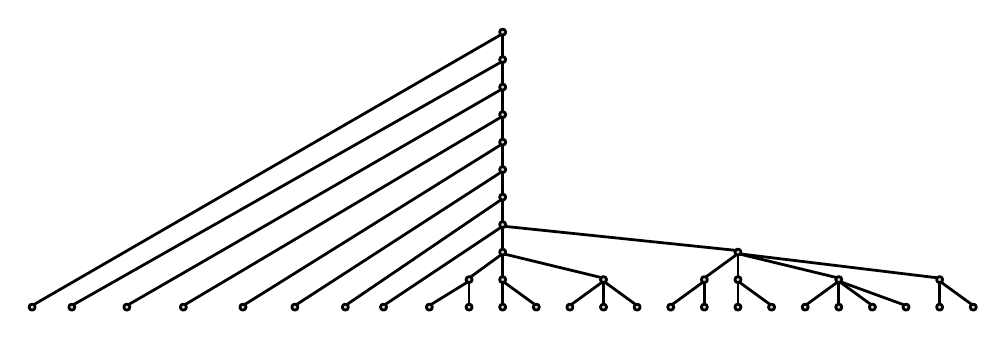
\begin{tikzpicture}[>=latex,line join=bevel,scale=0.55]
  \pgfsetlinewidth{1bp}
%%
\begin{scope}
  \pgfsetstrokecolor{black}
  \definecolor{strokecol}{rgb}{1.0,1.0,1.0};
  \pgfsetstrokecolor{strokecol}
  \definecolor{fillcol}{rgb}{1.0,1.0,1.0};
  \pgfsetfillcolor{fillcol}
  \filldraw (0bp,0bp) -- (0bp,184bp) -- (620bp,184bp) -- (620bp,0bp) -- cycle;
\end{scope}
\begin{scope}
  \pgfsetstrokecolor{black}
  \definecolor{strokecol}{rgb}{1.0,1.0,1.0};
  \pgfsetstrokecolor{strokecol}
  \definecolor{fillcol}{rgb}{1.0,1.0,1.0};
  \pgfsetfillcolor{fillcol}
  \filldraw (0bp,0bp) -- (0bp,184bp) -- (620bp,184bp) -- (620bp,0bp) -- cycle;
\end{scope}
\begin{scope}
  \pgfsetstrokecolor{black}
  \definecolor{strokecol}{rgb}{1.0,1.0,1.0};
  \pgfsetstrokecolor{strokecol}
  \definecolor{fillcol}{rgb}{1.0,1.0,1.0};
  \pgfsetfillcolor{fillcol}
  \filldraw (0bp,0bp) -- (0bp,184bp) -- (620bp,184bp) -- (620bp,0bp) -- cycle;
\end{scope}
  \pgfsetcolor{black}
  % Edge: c6 -> c7
  \draw [-] (308.67bp,126.21bp) .. controls (293.32bp,117.11bp) and (150.16bp,32.165bp)  .. (102.21bp,3.7204bp);
  % Edge: c14 -> c16
  \draw [-] (310bp,53.95bp) .. controls (310bp,53.137bp) and (310bp,51.914bp)  .. (310bp,40.075bp);
  % Edge: c2 -> c4
  \draw [-] (310bp,161.95bp) .. controls (310bp,161.14bp) and (310bp,159.91bp)  .. (310bp,148.07bp);
  % Edge: c23 -> c37
  \draw [-] (531.46bp,18.468bp) .. controls (536.27bp,16.722bp) and (551.85bp,11.054bp)  .. (572.49bp,3.5508bp);
  % Edge: c19 -> c40
  \draw [-] (311.18bp,18.14bp) .. controls (313.35bp,16.562bp) and (318.15bp,13.072bp)  .. (330.92bp,3.788bp);
  % Edge: c24 -> c38
  \draw [-] (596bp,17.95bp) .. controls (596bp,17.137bp) and (596bp,15.914bp)  .. (596bp,4.0746bp);
  % Edge: c20 -> c28
  \draw [-] (374.82bp,18.14bp) .. controls (372.65bp,16.562bp) and (367.85bp,13.072bp)  .. (355.08bp,3.788bp);
  % Edge: c17 -> c23
  \draw [-] (465.63bp,36.604bp) .. controls (472.77bp,34.873bp) and (501.67bp,27.869bp)  .. (528.18bp,21.44bp);
  % Edge: c4 -> c5
  \draw [-] (308.43bp,144.09bp) .. controls (290.18bp,133.56bp) and (118.2bp,34.287bp)  .. (65.429bp,3.825bp);
  % Edge: root -> c2
  \draw [-] (310bp,179.95bp) .. controls (310bp,179.14bp) and (310bp,177.91bp)  .. (310bp,166.07bp);
  % Edge: c14 -> c17
  \draw [-] (311.73bp,54.82bp) .. controls (325.55bp,53.384bp) and (418.45bp,43.732bp)  .. (462.08bp,39.199bp);
  % Edge: c8 -> c9
  \draw [-] (308.53bp,108.08bp) .. controls (294.48bp,99.323bp) and (183.68bp,30.237bp)  .. (141.32bp,3.8206bp);
  % Edge: c23 -> c34
  \draw [-] (528.82bp,18.14bp) .. controls (526.65bp,16.562bp) and (521.85bp,13.072bp)  .. (509.08bp,3.788bp);
  % Edge: c23 -> c36
  \draw [-] (531.18bp,18.14bp) .. controls (533.35bp,16.562bp) and (538.15bp,13.072bp)  .. (550.92bp,3.788bp);
  % Edge: c12 -> c13
  \draw [-] (308.84bp,72.214bp) .. controls (299.8bp,66.07bp) and (240.2bp,25.563bp)  .. (208.28bp,3.8724bp);
  % Edge: c6 -> c8
  \draw [-] (310bp,125.95bp) .. controls (310bp,125.14bp) and (310bp,123.91bp)  .. (310bp,112.07bp);
  % Edge: c20 -> c29
  \draw [-] (376bp,17.95bp) .. controls (376bp,17.137bp) and (376bp,15.914bp)  .. (376bp,4.0746bp);
  % Edge: c21 -> c32
  \draw [-] (442bp,17.95bp) .. controls (442bp,17.137bp) and (442bp,15.914bp)  .. (442bp,4.0746bp);
  % Edge: c20 -> c30
  \draw [-] (377.18bp,18.14bp) .. controls (379.35bp,16.562bp) and (384.15bp,13.072bp)  .. (396.92bp,3.788bp);
  % Edge: root -> c1
  \draw [-] (308.63bp,180.21bp) .. controls (288.9bp,168.81bp) and (62.55bp,37.993bp)  .. (3.2693bp,3.7336bp);
  % Edge: c17 -> c24
  \draw [-] (465.87bp,36.774bp) .. controls (478.74bp,35.213bp) and (554.77bp,25.997bp)  .. (594.38bp,21.196bp);
  % Edge: c10 -> c11
  \draw [-] (308.47bp,90.012bp) .. controls (296.16bp,82.046bp) and (212.84bp,28.132bp)  .. (175.35bp,3.871bp);
  % Edge: c4 -> c6
  \draw [-] (310bp,143.95bp) .. controls (310bp,143.14bp) and (310bp,141.91bp)  .. (310bp,130.07bp);
  % Edge: c12 -> c14
  \draw [-] (310bp,71.95bp) .. controls (310bp,71.137bp) and (310bp,69.914bp)  .. (310bp,58.075bp);
  % Edge: c23 -> c35
  \draw [-] (530bp,17.95bp) .. controls (530bp,17.137bp) and (530bp,15.914bp)  .. (530bp,4.0746bp);
  % Edge: c18 -> c26
  \draw [-] (288bp,17.95bp) .. controls (288bp,17.137bp) and (288bp,15.914bp)  .. (288bp,4.0746bp);
  % Edge: c8 -> c10
  \draw [-] (310bp,107.95bp) .. controls (310bp,107.14bp) and (310bp,105.91bp)  .. (310bp,94.075bp);
  % Edge: c17 -> c21
  \draw [-] (462.82bp,36.14bp) .. controls (460.65bp,34.562bp) and (455.85bp,31.072bp)  .. (443.08bp,21.788bp);
  % Edge: c16 -> c20
  \draw [-] (311.63bp,36.604bp) .. controls (318.77bp,34.873bp) and (347.67bp,27.869bp)  .. (374.18bp,21.44bp);
  % Edge: c22 -> c41
  \draw [-] (465.18bp,18.14bp) .. controls (467.35bp,16.562bp) and (472.15bp,13.072bp)  .. (484.92bp,3.788bp);
  % Edge: c22 -> c33
  \draw [-] (464bp,17.95bp) .. controls (464bp,17.137bp) and (464bp,15.914bp)  .. (464bp,4.0746bp);
  % Edge: c14 -> c15
  \draw [-] (308.9bp,54.265bp) .. controls (301.66bp,49.44bp) and (260.66bp,22.104bp)  .. (233.17bp,3.7831bp);
  % Edge: c16 -> c19
  \draw [-] (310bp,35.95bp) .. controls (310bp,35.137bp) and (310bp,33.914bp)  .. (310bp,22.075bp);
  % Edge: c18 -> c25
  \draw [-] (286.88bp,18.312bp) .. controls (284.32bp,16.738bp) and (277.82bp,12.734bp)  .. (263.33bp,3.8154bp);
  % Edge: c2 -> c3
  \draw [-] (308.74bp,162.29bp) .. controls (290.8bp,152.1bp) and (86.06bp,35.942bp)  .. (29.162bp,3.6594bp);
  % Edge: c10 -> c12
  \draw [-] (310bp,89.95bp) .. controls (310bp,89.137bp) and (310bp,87.914bp)  .. (310bp,76.075bp);
  % Edge: c24 -> c39
  \draw [-] (597.18bp,18.14bp) .. controls (599.35bp,16.562bp) and (604.15bp,13.072bp)  .. (616.92bp,3.788bp);
  % Edge: c16 -> c18
  \draw [-] (308.82bp,36.14bp) .. controls (306.65bp,34.562bp) and (301.85bp,31.072bp)  .. (289.08bp,21.788bp);
  % Edge: c17 -> c22
  \draw [-] (464bp,35.95bp) .. controls (464bp,35.137bp) and (464bp,33.914bp)  .. (464bp,22.075bp);
  % Edge: c21 -> c31
  \draw [-] (440.82bp,18.14bp) .. controls (438.65bp,16.562bp) and (433.85bp,13.072bp)  .. (421.08bp,3.788bp);
  % Edge: c19 -> c27
  \draw [-] (310bp,17.95bp) .. controls (310bp,17.137bp) and (310bp,15.914bp)  .. (310bp,4.0746bp);
  % Node: c10
\begin{scope}
  \definecolor{strokecol}{rgb}{0.0,0.0,0.0};
  \pgfsetstrokecolor{strokecol}
  \definecolor{fillcol}{rgb}{0.83,0.83,0.83};
  \pgfsetfillcolor{fillcol}
  \filldraw [opacity=1] (310bp,92bp) ellipse (2bp and 2bp);
\end{scope}
  % Node: c4
\begin{scope}
  \definecolor{strokecol}{rgb}{0.0,0.0,0.0};
  \pgfsetstrokecolor{strokecol}
  \definecolor{fillcol}{rgb}{0.83,0.83,0.83};
  \pgfsetfillcolor{fillcol}
  \filldraw [opacity=1] (310bp,146bp) ellipse (2bp and 2bp);
\end{scope}
  % Node: c2
\begin{scope}
  \definecolor{strokecol}{rgb}{0.0,0.0,0.0};
  \pgfsetstrokecolor{strokecol}
  \definecolor{fillcol}{rgb}{0.83,0.83,0.83};
  \pgfsetfillcolor{fillcol}
  \filldraw [opacity=1] (310bp,164bp) ellipse (2bp and 2bp);
\end{scope}
  % Node: c6
\begin{scope}
  \definecolor{strokecol}{rgb}{0.0,0.0,0.0};
  \pgfsetstrokecolor{strokecol}
  \definecolor{fillcol}{rgb}{0.83,0.83,0.83};
  \pgfsetfillcolor{fillcol}
  \filldraw [opacity=1] (310bp,128bp) ellipse (2bp and 2bp);
\end{scope}
  % Node: c19
\begin{scope}
  \definecolor{strokecol}{rgb}{0.0,0.0,0.0};
  \pgfsetstrokecolor{strokecol}
  \definecolor{fillcol}{rgb}{0.83,0.83,0.83};
  \pgfsetfillcolor{fillcol}
  \filldraw [opacity=1] (310bp,20bp) ellipse (2bp and 2bp);
\end{scope}
  % Node: c18
\begin{scope}
  \definecolor{strokecol}{rgb}{0.0,0.0,0.0};
  \pgfsetstrokecolor{strokecol}
  \definecolor{fillcol}{rgb}{0.83,0.83,0.83};
  \pgfsetfillcolor{fillcol}
  \filldraw [opacity=1] (288bp,20bp) ellipse (2bp and 2bp);
\end{scope}
  % Node: c39
\begin{scope}
  \definecolor{strokecol}{rgb}{0.0,0.0,0.0};
  \pgfsetstrokecolor{strokecol}
  \definecolor{fillcol}{rgb}{0.83,0.83,0.83};
  \pgfsetfillcolor{fillcol}
  \filldraw [opacity=1] (618bp,2bp) ellipse (2bp and 2bp);
\end{scope}
  % Node: c38
\begin{scope}
  \definecolor{strokecol}{rgb}{0.0,0.0,0.0};
  \pgfsetstrokecolor{strokecol}
  \definecolor{fillcol}{rgb}{0.83,0.83,0.83};
  \pgfsetfillcolor{fillcol}
  \filldraw [opacity=1] (596bp,2bp) ellipse (2bp and 2bp);
\end{scope}
  % Node: c13
\begin{scope}
  \definecolor{strokecol}{rgb}{0.0,0.0,0.0};
  \pgfsetstrokecolor{strokecol}
  \definecolor{fillcol}{rgb}{0.83,0.83,0.83};
  \pgfsetfillcolor{fillcol}
  \filldraw [opacity=1] (207bp,2bp) ellipse (2bp and 2bp);
\end{scope}
  % Node: c34
\begin{scope}
  \definecolor{strokecol}{rgb}{0.0,0.0,0.0};
  \pgfsetstrokecolor{strokecol}
  \definecolor{fillcol}{rgb}{0.83,0.83,0.83};
  \pgfsetfillcolor{fillcol}
  \filldraw [opacity=1] (508bp,2bp) ellipse (2bp and 2bp);
\end{scope}
  % Node: c11
\begin{scope}
  \definecolor{strokecol}{rgb}{0.0,0.0,0.0};
  \pgfsetstrokecolor{strokecol}
  \definecolor{fillcol}{rgb}{0.83,0.83,0.83};
  \pgfsetfillcolor{fillcol}
  \filldraw [opacity=1] (174bp,2bp) ellipse (2bp and 2bp);
\end{scope}
  % Node: c36
\begin{scope}
  \definecolor{strokecol}{rgb}{0.0,0.0,0.0};
  \pgfsetstrokecolor{strokecol}
  \definecolor{fillcol}{rgb}{0.83,0.83,0.83};
  \pgfsetfillcolor{fillcol}
  \filldraw [opacity=1] (552bp,2bp) ellipse (2bp and 2bp);
\end{scope}
  % Node: c17
\begin{scope}
  \definecolor{strokecol}{rgb}{0.0,0.0,0.0};
  \pgfsetstrokecolor{strokecol}
  \definecolor{fillcol}{rgb}{0.83,0.83,0.83};
  \pgfsetfillcolor{fillcol}
  \filldraw [opacity=1] (464bp,38bp) ellipse (2bp and 2bp);
\end{scope}
  % Node: c16
\begin{scope}
  \definecolor{strokecol}{rgb}{0.0,0.0,0.0};
  \pgfsetstrokecolor{strokecol}
  \definecolor{fillcol}{rgb}{0.83,0.83,0.83};
  \pgfsetfillcolor{fillcol}
  \filldraw [opacity=1] (310bp,38bp) ellipse (2bp and 2bp);
\end{scope}
  % Node: c15
\begin{scope}
  \definecolor{strokecol}{rgb}{0.0,0.0,0.0};
  \pgfsetstrokecolor{strokecol}
  \definecolor{fillcol}{rgb}{0.83,0.83,0.83};
  \pgfsetfillcolor{fillcol}
  \filldraw [opacity=1] (232bp,2bp) ellipse (2bp and 2bp);
\end{scope}
  % Node: c32
\begin{scope}
  \definecolor{strokecol}{rgb}{0.0,0.0,0.0};
  \pgfsetstrokecolor{strokecol}
  \definecolor{fillcol}{rgb}{0.83,0.83,0.83};
  \pgfsetfillcolor{fillcol}
  \filldraw [opacity=1] (442bp,2bp) ellipse (2bp and 2bp);
\end{scope}
  % Node: c35
\begin{scope}
  \definecolor{strokecol}{rgb}{0.0,0.0,0.0};
  \pgfsetstrokecolor{strokecol}
  \definecolor{fillcol}{rgb}{0.83,0.83,0.83};
  \pgfsetfillcolor{fillcol}
  \filldraw [opacity=1] (530bp,2bp) ellipse (2bp and 2bp);
\end{scope}
  % Node: c9
\begin{scope}
  \definecolor{strokecol}{rgb}{0.0,0.0,0.0};
  \pgfsetstrokecolor{strokecol}
  \definecolor{fillcol}{rgb}{0.83,0.83,0.83};
  \pgfsetfillcolor{fillcol}
  \filldraw [opacity=1] (140bp,2bp) ellipse (2bp and 2bp);
\end{scope}
  % Node: c8
\begin{scope}
  \definecolor{strokecol}{rgb}{0.0,0.0,0.0};
  \pgfsetstrokecolor{strokecol}
  \definecolor{fillcol}{rgb}{0.83,0.83,0.83};
  \pgfsetfillcolor{fillcol}
  \filldraw [opacity=1] (310bp,110bp) ellipse (2bp and 2bp);
\end{scope}
  % Node: c12
\begin{scope}
  \definecolor{strokecol}{rgb}{0.0,0.0,0.0};
  \pgfsetstrokecolor{strokecol}
  \definecolor{fillcol}{rgb}{0.83,0.83,0.83};
  \pgfsetfillcolor{fillcol}
  \filldraw [opacity=1] (310bp,74bp) ellipse (2bp and 2bp);
\end{scope}
  % Node: c3
\begin{scope}
  \definecolor{strokecol}{rgb}{0.0,0.0,0.0};
  \pgfsetstrokecolor{strokecol}
  \definecolor{fillcol}{rgb}{0.83,0.83,0.83};
  \pgfsetfillcolor{fillcol}
  \filldraw [opacity=1] (28bp,2bp) ellipse (2bp and 2bp);
\end{scope}
  % Node: c40
\begin{scope}
  \definecolor{strokecol}{rgb}{0.0,0.0,0.0};
  \pgfsetstrokecolor{strokecol}
  \definecolor{fillcol}{rgb}{0.83,0.83,0.83};
  \pgfsetfillcolor{fillcol}
  \filldraw [opacity=1] (332bp,2bp) ellipse (2bp and 2bp);
\end{scope}
  % Node: c1
\begin{scope}
  \definecolor{strokecol}{rgb}{0.0,0.0,0.0};
  \pgfsetstrokecolor{strokecol}
  \definecolor{fillcol}{rgb}{0.83,0.83,0.83};
  \pgfsetfillcolor{fillcol}
  \filldraw [opacity=1] (2bp,2bp) ellipse (2bp and 2bp);
\end{scope}
  % Node: c7
\begin{scope}
  \definecolor{strokecol}{rgb}{0.0,0.0,0.0};
  \pgfsetstrokecolor{strokecol}
  \definecolor{fillcol}{rgb}{0.83,0.83,0.83};
  \pgfsetfillcolor{fillcol}
  \filldraw [opacity=1] (101bp,2bp) ellipse (2bp and 2bp);
\end{scope}
  % Node: c37
\begin{scope}
  \definecolor{strokecol}{rgb}{0.0,0.0,0.0};
  \pgfsetstrokecolor{strokecol}
  \definecolor{fillcol}{rgb}{0.83,0.83,0.83};
  \pgfsetfillcolor{fillcol}
  \filldraw [opacity=1] (574bp,2bp) ellipse (2bp and 2bp);
\end{scope}
  % Node: c5
\begin{scope}
  \definecolor{strokecol}{rgb}{0.0,0.0,0.0};
  \pgfsetstrokecolor{strokecol}
  \definecolor{fillcol}{rgb}{0.83,0.83,0.83};
  \pgfsetfillcolor{fillcol}
  \filldraw [opacity=1] (64bp,2bp) ellipse (2bp and 2bp);
\end{scope}
  % Node: c41
\begin{scope}
  \definecolor{strokecol}{rgb}{0.0,0.0,0.0};
  \pgfsetstrokecolor{strokecol}
  \definecolor{fillcol}{rgb}{0.83,0.83,0.83};
  \pgfsetfillcolor{fillcol}
  \filldraw [opacity=1] (486bp,2bp) ellipse (2bp and 2bp);
\end{scope}
  % Node: c22
\begin{scope}
  \definecolor{strokecol}{rgb}{0.0,0.0,0.0};
  \pgfsetstrokecolor{strokecol}
  \definecolor{fillcol}{rgb}{0.83,0.83,0.83};
  \pgfsetfillcolor{fillcol}
  \filldraw [opacity=1] (464bp,20bp) ellipse (2bp and 2bp);
\end{scope}
  % Node: c23
\begin{scope}
  \definecolor{strokecol}{rgb}{0.0,0.0,0.0};
  \pgfsetstrokecolor{strokecol}
  \definecolor{fillcol}{rgb}{0.83,0.83,0.83};
  \pgfsetfillcolor{fillcol}
  \filldraw [opacity=1] (530bp,20bp) ellipse (2bp and 2bp);
\end{scope}
  % Node: c20
\begin{scope}
  \definecolor{strokecol}{rgb}{0.0,0.0,0.0};
  \pgfsetstrokecolor{strokecol}
  \definecolor{fillcol}{rgb}{0.83,0.83,0.83};
  \pgfsetfillcolor{fillcol}
  \filldraw [opacity=1] (376bp,20bp) ellipse (2bp and 2bp);
\end{scope}
  % Node: c21
\begin{scope}
  \definecolor{strokecol}{rgb}{0.0,0.0,0.0};
  \pgfsetstrokecolor{strokecol}
  \definecolor{fillcol}{rgb}{0.83,0.83,0.83};
  \pgfsetfillcolor{fillcol}
  \filldraw [opacity=1] (442bp,20bp) ellipse (2bp and 2bp);
\end{scope}
  % Node: c26
\begin{scope}
  \definecolor{strokecol}{rgb}{0.0,0.0,0.0};
  \pgfsetstrokecolor{strokecol}
  \definecolor{fillcol}{rgb}{0.83,0.83,0.83};
  \pgfsetfillcolor{fillcol}
  \filldraw [opacity=1] (288bp,2bp) ellipse (2bp and 2bp);
\end{scope}
  % Node: c27
\begin{scope}
  \definecolor{strokecol}{rgb}{0.0,0.0,0.0};
  \pgfsetstrokecolor{strokecol}
  \definecolor{fillcol}{rgb}{0.83,0.83,0.83};
  \pgfsetfillcolor{fillcol}
  \filldraw [opacity=1] (310bp,2bp) ellipse (2bp and 2bp);
\end{scope}
  % Node: c24
\begin{scope}
  \definecolor{strokecol}{rgb}{0.0,0.0,0.0};
  \pgfsetstrokecolor{strokecol}
  \definecolor{fillcol}{rgb}{0.83,0.83,0.83};
  \pgfsetfillcolor{fillcol}
  \filldraw [opacity=1] (596bp,20bp) ellipse (2bp and 2bp);
\end{scope}
  % Node: c25
\begin{scope}
  \definecolor{strokecol}{rgb}{0.0,0.0,0.0};
  \pgfsetstrokecolor{strokecol}
  \definecolor{fillcol}{rgb}{0.83,0.83,0.83};
  \pgfsetfillcolor{fillcol}
  \filldraw [opacity=1] (262bp,2bp) ellipse (2bp and 2bp);
\end{scope}
  % Node: c31
\begin{scope}
  \definecolor{strokecol}{rgb}{0.0,0.0,0.0};
  \pgfsetstrokecolor{strokecol}
  \definecolor{fillcol}{rgb}{0.83,0.83,0.83};
  \pgfsetfillcolor{fillcol}
  \filldraw [opacity=1] (420bp,2bp) ellipse (2bp and 2bp);
\end{scope}
  % Node: c28
\begin{scope}
  \definecolor{strokecol}{rgb}{0.0,0.0,0.0};
  \pgfsetstrokecolor{strokecol}
  \definecolor{fillcol}{rgb}{0.83,0.83,0.83};
  \pgfsetfillcolor{fillcol}
  \filldraw [opacity=1] (354bp,2bp) ellipse (2bp and 2bp);
\end{scope}
  % Node: c29
\begin{scope}
  \definecolor{strokecol}{rgb}{0.0,0.0,0.0};
  \pgfsetstrokecolor{strokecol}
  \definecolor{fillcol}{rgb}{0.83,0.83,0.83};
  \pgfsetfillcolor{fillcol}
  \filldraw [opacity=1] (376bp,2bp) ellipse (2bp and 2bp);
\end{scope}
  % Node: c30
\begin{scope}
  \definecolor{strokecol}{rgb}{0.0,0.0,0.0};
  \pgfsetstrokecolor{strokecol}
  \definecolor{fillcol}{rgb}{0.83,0.83,0.83};
  \pgfsetfillcolor{fillcol}
  \filldraw [opacity=1] (398bp,2bp) ellipse (2bp and 2bp);
\end{scope}
  % Node: c33
\begin{scope}
  \definecolor{strokecol}{rgb}{0.0,0.0,0.0};
  \pgfsetstrokecolor{strokecol}
  \definecolor{fillcol}{rgb}{0.83,0.83,0.83};
  \pgfsetfillcolor{fillcol}
  \filldraw [opacity=1] (464bp,2bp) ellipse (2bp and 2bp);
\end{scope}
  % Node: c14
\begin{scope}
  \definecolor{strokecol}{rgb}{0.0,0.0,0.0};
  \pgfsetstrokecolor{strokecol}
  \definecolor{fillcol}{rgb}{0.83,0.83,0.83};
  \pgfsetfillcolor{fillcol}
  \filldraw [opacity=1] (310bp,56bp) ellipse (2bp and 2bp);
\end{scope}
  % Node: root
\begin{scope}
  \definecolor{strokecol}{rgb}{0.0,0.0,0.0};
  \pgfsetstrokecolor{strokecol}
  \definecolor{fillcol}{rgb}{0.83,0.83,0.83};
  \pgfsetfillcolor{fillcol}
  \filldraw [opacity=1] (310bp,182bp) ellipse (2bp and 2bp);
\end{scope}
%
\end{tikzpicture}


\end{center}
\caption{A badly-drawn multiple-outlier cover tree.}
\label{fig:outliers}
\end{figure}

A tree that has this chain-like structure all the way down is going to perform
horrendously; motivated by this observation, we define a measure of tree
imbalance.

\begin{defn}
The {\it cover node imbalance} $i(\mathscr{N}_i)$ for a cover tree node
$\mathscr{N}_i$ with scale $s_i$ in the cover tree $\mathscr{T}$ is defined as
the cumulative number of missing levels between the node and its parent
$\mathscr{N}_p$ (which has scale $s_p$).  If
the node is a leaf child (that is, $s_i = -\infty$), then number of missing
levels is defined as the difference between $s_p$ and $s_{\min} - 1$ where
$s_{\min}$ is the smallest scale of a non-leaf node in $\mathscr{T}$.  If
$\mathscr{N}_i$ is the root of the tree, then the cover node imbalance is 0.
Explicitly written, this calculation is

\begin{equation}
i(\mathscr{N}_i) = \begin{dcases*}
  s_p - s_i - 1 & if $\mathscr{N}_i$ is not a leaf and not the root node \\
  \max(s_p - s_{\min} - 1, \; 0) & if $\mathscr{N}_i$ is a leaf \\
  0 & if $\mathscr{N}_i$ is the root node.
  \end{dcases*}
\end{equation}
\end{defn}

This simple definition of cover node imbalance is easy to calculate, and using
it, we can generalize to a measure of imbalance for the full tree.

\begin{defn}
The {\it cover tree imbalance} $b(\mathscr{T})$ for a cover tree $\mathscr{T}$
is defined as the cumulative number of missing levels in the tree.  This can be
expressed as a function of cover node imbalances easily:

\begin{equation}
b(\mathscr{T}) = \sum_{\mathscr{N}_i \in \mathscr{T}} i(\mathscr{N}_i).
\end{equation}
\end{defn}

A perfectly balanced cover tree $\mathscr{T}_b$ with no missing levels has
imbalance $i(\mathscr{T}_b) = 0$ (for instance, Figure
\ref{fig:imbalance-good}).  A worst-case cover tree $\mathscr{T}_w$ which is
entirely a chain-like structure with maximum scale $s_{\max}$ and minimum scale
$s_{\min}$ will have imbalance $i(\mathscr{T}_w) \sim N (s_{\max} - s_{\min})$.
Because of this chain-like structure, each level has only one node and thus
there are at least $N$ levels; or, $s_{\max} - s_{\min} \ge N$, meaning that the
imbalance is actually quadratic in $N$!

As we will see later empirically, the notion of cover tree imbalance does a good
job of capturing the `goodness' of a tree.  We will use this notion in order to
quantify the worst-case performance of dual-tree algorithms using the cover
tree.

{\bf TODO: Can any bound be proven on $i(\mathscr{T})$?  I haven't thought of
anything successfully yet.}


\section{General runtime bound}
\label{sec:bound}

\begin{thm}
\label{thm:ct-runtime}
%For any dual-tree algorithm using cover trees and the standard cover tree
%dual-tree pruning traversal (Algorithm \ref{alg:cover-tree-dual}) with reference
%set $S_r$ that has expansion constant $c_r$ and query set $S_q$, the runtime is
%bounded above by $O(c_r^4 | R^* | \nu \chi \psi N)$, where $ | R^* | $ is
%the maximum size of the reference set $R$ (line
%\ref{alg:line:ct-dual-input}) at any point in the dual-tree pruning traversal,
%$\chi$ is the longest possible running time of \texttt{BaseCase()}, and $\psi$
%is the longest possible running time of \texttt{Score()}.
Given a reference set $S_r$ of size $N$ with an expansion constant $c_r$ and a
set of queries $S_q$ of size $O(N)$, a standard cover tree based dual-tree
algorithm (Algorithm \ref{alg:cover-tree-dual}) takes $O(c_r^4 | R^* | \nu \chi
\psi N)$, where $ | R^* | $ is the maximum size of the reference set $R$ (line
\ref{alg:line:ct-dual-input}) during the dual-tree recursion, $\chi$ is
the maximum possible runtime of \texttt{BaseCase()}, and $\psi$ is the maximum
possible runtime of \texttt{Score()}.
\end{thm}

\vspace*{-1.23em}
\begin{proof}
Consider a reference recursion (lines
\ref{alg:line:ct-dual-ref-recursion-start}--\ref{alg:line:ct-dual-ref-recursion-end}).
The work done in the base case loop from lines
\ref{alg:line:ct-dual-base-case-start}--\ref{alg:line:ct-dual-base-case-end} is
$O(\chi | R |)$.  Define $| R^* |$ to be the largest set $|R|$ for any scale
$s_r^{\max}$ and any query node $\mathscr{N}_q$ during the course of the
algorithm; then, it is true that $| R | \le | R^* |$.
%
Then, lines \ref{alg:line:ct-dual-ref-children} and
\ref{alg:line:ct-dual-ref-score} take $O(c_r^4 \psi | R |) \le O(c_r^4 \psi |
R^* |)$ time, because each reference node has $c_r^4$ children.  So, one
full reference recursion takes $O(c_r^4 \psi | R^* |)$ time.

Now, note that there are $O(N)$ nodes in $\mathscr{T}_q$.  Thus, line
\ref{alg:line:ct-dual-query-recursion} is visited $O(N)$ times.  Each of these
$O(N)$ visits to line \ref{alg:line:ct-dual-query-recursion} implies a
recursion, in which the reference set is descended up to $\nu$ times (lines
\ref{alg:line:ct-dual-ref-recursion-start}--\ref{alg:line:ct-dual-ref-recursion-end})
before the query node is descended or the algorithm terminates.  In addition,
each $O(N)$ recursion implies an $O(\psi |R|) \le O(\psi |R^*|)$ operation for
the calculation of $R'$ (line \ref{alg:line:ct-dual-query-pruning}).  Thus, the
full runtime of the algorithm is bounded as $O(c_r^4 |R^*| \nu \chi \psi N +
\psi |R^*| N) = O(c_r^4 |R^*| \nu \chi \psi N)$.
\end{proof}
\vspace*{-0.8em}

This result holds for any dual-tree algorithm regardless of the problem. Hence,
%for any pairwise statistical problem, the runtime of the dual-tree algorithm (of
the runtime of any dual-tree algorithm
%that problem)
would be at least $O(N)$ using our bound, which matches the intuition that
answering $O(N)$ queries would take at least $O(N)$ time. For a particular
problem and data, if $c_r$, $|R^*|$, $\nu$, $\chi$ and
$\psi$ are bounded by constants independent of $N$ (for large enough $N$), then
the dual-tree algorithm for that problem has a runtime linear in $N$. Our
theoretical result separates out the problem-dependent and the
problem-independent elements of the runtime bound, which allows us to simply
plug in the problem-dependent bounds to get runtime bounds for any dual-tree
algorithm without requiring an analysis from scratch.
% This discussion already happened earlier... sort of.
%The expansion constant is related to a notion of intrinsic dimensionality of a
%dataset (as discussed earlier). A relatively small $c_r$ corresponds to
%a dataset with low intrinsic dimensionality, while a value of $c_r$ independent
%of $N$ implies that the intrinsic dimensionality of the data is independent of
%the number of points in the dataset. The latter is a reasonable assumption in
%many scenarios.
%Our bound has a linear dependence on the inverse constant of bichromaticity
%$\nu$; this results from the worst-case situation where the reference tree is
%recursed entirely after all query tree recursions
% this makes sense, given that $\nu$ represents the maximum number of times
%any set $R$ is descended for any query node $\mathscr{N}_q$ before
%$\mathscr{N}_q$ is recursed.
If $\nu \sim \kappa$, which is a reasonable assumption, this is a better result
than the results of Ram et.~al.  \cite{ram2009} who found a dependence of
$c_q^{4 \kappa}$ in their proofs.

The quantity $|R^*|$ bounds the amount of work that needs to be done for each
recursion. In the worst case, $|R^*|$ can be $N$. However,
dual-tree algorithms rely on branch-and-bound techniques to prune away
work (Lines \ref{alg:line:ct-dual-ref-score} and
\ref{alg:line:ct-dual-query-pruning} in Algorithm \ref{alg:cover-tree-dual}). A
small value of $|R^*|$ will imply that the algorithm is extremely successful in
pruning away work at Line \ref{alg:line:ct-dual-ref-score} in Algorithm
\ref{alg:cover-tree-dual}. An (upper) bound on $|R^*|$ (and the algorithm's
success in pruning work) will depend on the problem and the data.  As we will
show, bounding $|R^*|$ is often possible. % In addition, we will also show that
For many dual-tree algorithms, $\chi \sim \psi \sim O(1)$; often, cached
sufficient statistics~\cite{moore2000anchors} can enable $O(1)$ runtime
implementations of \texttt{BaseCase()} and \texttt{Score()}.

% Space constraints :(

%The runtime bound $\chi$ for the \texttt{BaseCase($p_q$, $p_r$)} function
%corresponds to the time required to process a pair of points. For example, in
%range search, \texttt{BaseCase()} corresponds to the
%time taken to compute $d(p_q, p_r)$ and determine if that falls into the desired
%range.  For general kernel summations, this corresponds to computing the
%pairwise kernel function between $p_q$ and $p_r$ and then summing it to the
%output for $p_q$.  In general, the runtime of \texttt{BaseCase()} is dominated
%by the pairwise function computation which is independent of $N$ and is usually
%$O(1)$. The \texttt{Score()} function is an operation on a pair of nodes and
%usually involves computing a bound which requires a pairwise function
%computation between the node centers (similar to the \texttt{BaseCase()}
%function except that it is for node centres) and certain cached node statistics
%(such as node radius in the metric space). Hence its runtime bound $\psi$ is
%usually a constant independent of $N$ or simply $O(1)$.


\section{Nearest neighbor search}
\label{sec:nns}

%\begin{minipage}{0.4\textwidth}
\begin{algorithm}[tb]
%\begin{subfigure}[b]{0.48\textwidth}
%  \SetAlgoLined
\begin{algorithmic}
    \STATE {\bfseries Input:} query point $p_q$, reference point $p_r$, list of
candidate neighbors $N$ and distances $D$
    \STATE {\bfseries Output:} distance $d$ between $p_q$ and $p_r$

    \medskip
%    \STATE $d \gets \| p_q - p_r \|$
%    \medskip

    \IF{$d(p_q, p_r) < D[p_q]$ \AND \texttt{BaseCase($p_q$, $p_r$)} not yet called}
    \STATE  $D[p_q] \gets d(p_q, p_r)$, and $N[p_q] \gets p_r$
    \ENDIF

    \RETURN $d(p_q, p_r)$
  \end{algorithmic}

  \caption{Nearest neighbor search \texttt{BaseCase()}}
  \label{alg:nn_base_case}
%\end{subfigure}
\end{algorithm}
%\end{minipage}

%\begin{subfigure}[b]{0.48\textwidth}
%\begin{minipage}{0.4\textwidth}
\begin{algorithm}[tb]
  \begin{algorithmic}
    \STATE {\bfseries Input:} query node $\mathscr{N}_q$, reference node
$\mathscr{N}_r$
    \STATE {\bfseries Output:} a score for the node combination $(\mathscr{N}_q,
\mathscr{N}_r)$, or $\infty$ if the combination should be pruned

    \medskip

    \IF{$d_{\min}(\mathscr{N}_q, \mathscr{N}_r) < B(\mathscr{N}_q)$}
      \RETURN $d_{\min}(\mathscr{N}_q, \mathscr{N}_r)$
    \ENDIF

%    \medskip
    \RETURN $\infty$
  \end{algorithmic}

  \caption{Nearest neighbor search \texttt{Score()}}
  \label{alg:nn_score}
\end{algorithm}
%\end{minipage}
%\end{subfigure}
%\end{figure}

The standard task of nearest neighbor search can be simply described: given a
query set $S_q$ and a reference set $S_r$, for each query point $p_q \in S_q$,
find the nearest neighbor $p_r$ in the reference set $S_r$.  The task is
well-studied and well-known, and there exist numerous approaches for both exact
and approximate nearest neighbor search, including the cover tree nearest
neighbor search algorithm due to \citet{langford2006}.  We will consider that
algorithm, but in a tree-independent sense as given by \citet{curtin2013tree};
this means that to describe the algorithm, we require only a \texttt{BaseCase()}
and \texttt{Score()} function; these are given in Algorithms
\ref{alg:nn_base_case} and \ref{alg:nn_score}, respectively.

Given a type of tree and traversal, these two functions store the current
nearest neighbor candidates in the array $N$ and their distances in the array
$D$. \citep[see][for a more complete
discussion of how this algorithm works and a proof of
correctness.]{curtin2013tree}  The
\texttt{Score()} function depends on a bound function $B(\mathscr{N}_q)$ which
represents the maximum distance that could possibly improve a nearest neighbor
candidate for any descendant point of the query node $\mathscr{N}_q$.  The
standard bound function $B(\mathscr{N}_q)$ used for cover trees is
%\begin{equation}
$B(\mathscr{N}_q) \le D[p_q] + 2^{s_q + 1}$ \citep[this is adapted from][]{langford2006}.
%\end{equation}

%\begin{figure}

%\begin{equation}
%\begin{split}
%B(\mathscr{N}_q) = \min &\left\{ \max \big\{ \max_{p \in \mathscr{P}_q}
%D[p], \max_{\mathscr{N}_c \in \mathscr{C}_q} B(\mathscr{N}_c) \big\},
%\right. \\
% & \left. \min_{p \in \mathscr{P}_q} \big(D[p] + \rho(\mathscr{N}_q) +
%\lambda(\mathscr{N}_q)\big)
%,\right. \\
% & \left. \min_{\mathscr{N}_c \in \mathscr{C}_q} \Big(B(\mathscr{N}_c) + 2
%\big(\lambda(\mathscr{N}_q) - \lambda(\mathscr{N}_c)\big)\Big) \right. \\
% & B(\operatorname{Par}(\mathscr{N}_q)) \bigg\} . \\
%\end{split}
%\end{equation}

%Although that is a particularly complex definition, what we'll be talking about
%is only cover trees, and we can relax the bound a bit:

%\begin{eqnarray}
%B(\mathscr{N}_q) &\le& \min_{p \in \mathscr{P}_q} \big(D[p] +
%\rho(\mathscr{N}_q) + \lambda(\mathscr{N}_q) \big) \\
% &=& \min_{p \in \mathscr{P}_q} \big(D[p] + \lambda(\mathscr{N}_q) \big) \\
% &=& D[p_q] + \lambda(\mathscr{N}_q) \\
% &=& D[p_q] + 2^{s_q + 1} \\
%&=:& B_c(\mathscr{N}_q).
%\end{eqnarray}

In this formulation, the query node $\mathscr{N}_q$ holds the the query point
$p_q$, the quantity $D[p_q]$ is the current nearest neighbor candidate distance
for the query point $p_q$, and $2^{s_q + 1}$ corresponds to the furthest
descendant distance of $\mathscr{N}_q$.  For notational convenience in the
following proof, take $c_{qr} = \max((\max_{p_q \in S_q} c'_r), c_r)$, where
$c'_r$ is the expansion constant of the set $S_r \cup \{ p_q \}$.

%This follows because $\rho(\mathscr{N}_q) = 0$ for all cover tree
%nodes because each cover tree node only holds one point and that point is the
%centroid of the node.  Also, for a cover tree node $\mathscr{N}_i$ with scale
%$s_i$,

%\begin{equation}
%\label{eqn:ct-fdd-bound}
%\lambda(\mathscr{N}_i) \le 2^{s_i + 1}.
%\end{equation}

\begin{thm}
Using cover trees, the standard cover tree pruning dual-tree traversal, and the
nearest neighbor search \texttt{BaseCase()} and \texttt{Score()} as given in
Algorithms \ref{alg:nn_base_case} and \ref{alg:nn_score}, respectively, and also
given a reference set $S_r$ with expansion constant $c_r$, a query set $S_q$,
the running time of the algorithm is bounded by $O(c_r^4 c_{qr}^5 (N + \theta))$
with $\theta$ defined as in Theorem \ref{thm:ct-runtime}.
\label{thm:nns}
\end{thm}

\begin{proof}
The running time of \texttt{BaseCase()} and \texttt{Score()} are clearly $O(1)$.
Due to Theorem \ref{thm:ct-runtime}, we therefore know that the runtime of the
algorithm is bounded by $O(c_r^4 |R^*| (N + \theta))$.  Thus, the only thing
that remains is to bound the maximum size of the reference set, $|R^*|$.

Assume that when $R^*$ is encountered, the maximum reference scale is
$s_r^{\max}$ and the query node is $\mathscr{N}_q$.  Every node $\mathscr{N}_r
\in R^*$ satisfies the property enforced in line
\ref{alg:line:ct-dual-ref-score} that
%\begin{equation}
$d_{\min}(\mathscr{N}_q, \mathscr{N}_r) \le B(\mathscr{N}_q)$.
%\end{equation}
%Relaxing this slightly,
%\begin{equation}
%d_{\min}(\mathscr{N}_q, \mathscr{N}_r) \le B_c(\mathscr{N}_q).
%\end{equation}
Using the definition of $d_{\min}(\cdot, \cdot)$ and $B(\cdot)$, we
expand the equation.  Note that $p_q$ is the point held in $\mathscr{N}_q$ and
$p_r$ is the point held in $\mathscr{N}_r$.  Also, take $\hat{p}_r$ to be the
current nearest neighbor candidate for $p_q$; that is, $D[p_q] = d(p_q,
\hat{p}_r)$.  Then,

\begin{eqnarray}
%d(p_q, p_r) - \lambda(\mathscr{N}_q) - \lambda(\mathscr{N}_r) &\le& D[p_q] +
%2^{s_q + 1} \\
%d(p_q, p_r) &\le& d(p_q, \hat{p}_r) + \lambda(\mathscr{N}_q) +
%\lambda(\mathscr{N}_r) + 2^{s_q + 1} \\
%d(p_q, p_r) - 2^{s_q + 1} - 2^{s_r + 1} &\le& D[p_q] + 2^{s_q + 1} \\
d(p_q, p_r) &\le& d(p_q, \hat{p}_r) + 2^{s_q + 1} + 2^{s_r + 1} + 2^{s_q + 1}
\label{eqn:pr_dist} \\
 &\le& d(p_q, \hat{p}_r) + 2(2^{s_r^{\max} + 1})
\end{eqnarray}

\noindent where the last step follows because $s_q + 1 \le s_r^{\max}$ and $s_r
\le s_r^{\max}$.  Define the set of points $P$ as the points held in each node
in $R^*$ (that is, $P = \{ p_r \in \mathscr{P}(\mathscr{N}_r) : \mathscr{N}_r
\in R^* \}$).  Then, we can write

%\begin{equation}
% = \{ p_r : \mathscr{N}_r \in \mathscr{C}(\mathscr{N}_p), \; s_p = s_r^{\max} + 1 \}.
%\end{equation}
%
%  Stated differently, we have that each point $p_r$ for each node
%$\mathscr{N}_r \in R$ is such that

\begin{equation}
P \subseteq B_{S_r}(p_q, d(p_q, \hat{p}_r) + 2(2^{s_r^{\max} + 1}))
\end{equation}

%\noindent or that

%\begin{equation}
%R \subseteq B_{S_r}(p_q, d(p_q, \hat{p}_r) + 3(2^{s_r^{\max} + 1})).
%\end{equation}

Suppose that the true nearest neighbor is $p_r^*$ and $d(p_q, p_r^*) >
2^{s_r^{\max} + 1}$.  Then, $p_r^*$ must be held as a descendant point of some
node in $R^*$ which holds some point $\tilde{p}_r$.  Using the triangle
inequality,

%\begin{eqnarray}
\begin{equation}
d(p_q, \hat{p}_r) \le d(p_q, \tilde{p}_r)
 \le d(p_q, p_r^*) + d(\tilde{p}_r, p_r^*)
 \le d(p_q, p_r^*) + 2^{s_r^{\max} + 1}.
%\end{eqnarray}
\end{equation}

This gives that
%\begin{equation}
$P \subseteq B_{S_r \cup \{ p_q \}}(p_q, d(p_q, p_r^*) + 3(2^{s_r^{\max} +
1}))$.
% &\subseteq& B_{S_r \cup \{ p_q \}}(p_q, d(p_q, p_r^*) + 3(2^{s_r^{\max} + 1}))
%\end{equation}
The previous step is necessary: to apply the definition of the expansion
constant, the ball must be centered at a point in the set; now, the center
($p_q$) is part of the set.

\begin{eqnarray}
| B_{S_r \cup \{ p_q \}}(p_q, d(p_q, p_r^*) + 3(2^{s_r^{\max} + 1})) | &\le& |
B_{S_r \cup \{ p_q \}}(p_q, 4 d(p_q, p_r^*)) | \\
% &\le& | B_{S_{qr}}(p_q, 8 d(p_q, p_r^*)) | \\
% &\le& (c'_r)^3 | B_{S_r \cup \{ p_q \}}(p_q, d(p_q, p_r^*) / 2) | \\
 &\le& c_{qr}^3 | B_{S_r \cup \{ p_q \}}(p_q, d(p_q, p_r^*) / 2 |
\end{eqnarray}

\noindent which follows because the expansion constant of the set $S_r \cup \{
p_q \}$ is bounded above by $c_{qr}$.  Next, we know that $p_r^*$ is the closest
point to $p_q$ in $S_r \cup \{ p_q \}$; thus, there cannot exist a point $p'_r
\ne p_q \in S_r \cup \{ p_q \}$ such that
%\begin{equation}
$p'_r \in B_{S_{qr}}(p_q, d(p_q, p_r^*) / 2)$
%\end{equation}
because that would imply that $d(p_q, p'_r) < d(p_q, p_r^*)$, which is
a contradiction.  Thus, the only point in the ball is $p_q$, and we have that $|
B_{S_r \cup \{ p_q \}}(p_q, d(p_q, p_r^*) / 2) | = 1$, giving the result that
$|R| \le c_{qr}^3$ in this case.

%%%%%%%%

% Changes from below by Pari are applied.

%****************************************************

%Again, I think the proof from Eq 18 onwards is incorrect. If $B_{S_{qr}}(p_q, \cdot)$ is infact the ball around the data, then $|B_{S_{qr}}(p_q, d(p_q, \hat{p}_r) / 2)| \not= 1$. This would hold only for the actual nearest-neighbor of $p_q$, not any neighbor candidate. If you mean that $B_{S_{qr}}(p_q, \cdot)$ is infact the intersection of the ball around the data and the set of all (implicit) nodes at scale $s_r^{\max}$, then the definition of expansion constant (as in Eq 19) cannot be applied to that set. It can only be applied to the actual ball around the data.

%The fix is straightforward though -- you just have to replace $\hat{p}_r$ with $p_r^*$, the true nearest neighbour of $p_q$. Now $\hat{p}_r$ at least has an implicit node at scale $s_r^{\max}$. Let $\tilde{p}_r$ be the node at scale $s_r^{\max}$ which contains $p_r^*$ as a descendant. So $\tilde{p}_r$'s farthest descendant is at most $2^{s_r^{\max} + 1}$ away from it. So it follows that:
%\begin{eqnarray*}
%d(p_q, \hat{p}_r) & \leq & d(p_q, \tilde{p}_r) \mbox{ since $\hat{p}_r$ is the current closest, } \\
% & \leq & d(p_q, p_r^*) + d(\tilde{p}_r, p_r^*) \mbox{ by triangle inequality, } \\
% & \leq & d(p_q, p_r^*) + 2^{s_r^{\max} + 1}.
%\end{eqnarray*}
%Now you can say that
%$$B_{S_{qr}}(p_q, d(p_q, \hat{p}_r) + 3(2^{s_r^{\max} + 1})) \subseteq B_{S_{qr}}(p_q, d(p_q, p_r^*) + 2^{s_r^{\max} + 1} + 3(2^{s_r^{\max} + 1})),$$
%and work with the right hand side ball and use the argument that $|B_{S_{qr}}(p_q, d(p_q, p_r^*) / 2)| = 1$.


%****************************************************

%%%%%%%%

The other case is when $d(p_q, p_r^*) \le 2^{s_r^{\max} + 1}$, which means that
$d(p_q, \hat{p}_r) \le 2^{s_r^{\max} + 2}$. %  We use a packing argument,
%similar to the proof of Lemma~4.1 in \cite{langford2006}.
Note that $P \in C_{s_r^{\max}}$, and therefore

\begin{eqnarray}
P &\subseteq& B_{S_r}(p_q, d(p_q, p_r^*) + 3(2^{s_r^{\max} + 1})) \cap
C_{s_r^{\max}} \\
 &\subseteq& B_{S_r}(p_q, 4(2^{s_r^{\max} + 1})) \cap C_{s_r^{\max}}.
\end{eqnarray}

Every point in $C_{s_r^{\max}}$ is separated by at least $2^{s_r^{\max}}$.
Using Lemma \ref{lem:packing} with $\delta = 2^{s_r^{\max}}$ and $\rho = 8$
yields that $|P| \le c_r^5$.  This gives the result, because $c_r^5 \le
c_{qr}^5$.
\end{proof}

%By assumption (and Equation \ref{eqn:pr_dist}), for any $p_r \in
%P$,
%\begin{equation}
%$d(p_q, p_r) \leq 2^{s_r^{\max} + 3}$.
%\end{equation}
%Therefore, for any such $p_r$,

%\begin{eqnarray}
%\begin{equation}
%B_{S_r} \left( p_q, d(p_q, p_r^*) + 3(2^{s_r^{\max} + 1}) \right) \subseteq
%B_{S_r} \left( p_q, 2^{s_r^{\max} + 3} \right)
% \subseteq B_{S_r} \left(p_r, 2^{s_r^{\max} + 4} \right).
% &\subseteq& B_{S_r} \left(p_r, 2^{s_r^{\max} + 4} \right).
%\end{eqnarray}
%\end{equation}

%Applying the definition of $c_r$, we have that
%\begin{equation}
%$| B_{S_r} (p_r, 2^{s_r^{\max} + 4} ) | \leq c_r^5 | B_{S_r} (p_r,
%2^{s_r^{\max}-1} ) |$.
%\label{eqn:packing1}
%\end{equation}

%Any two points corresponding to nodes in $R^*$ are separated by at least
%$2^{s_r^{\max}}$, so each ball
%can  contain only one node in $R^*$. Therefore, the total
%number of nodes in $R^*$ is bounded by the number of disjoint balls of size
%$2^{s_r^{\max} - 1}$ that can be packed into a ball of size $2^{s_r^{\max} +
%4}$.
%
%In the worst case, this packing is perfect, and we have that
%\begin{equation}
%|B_{S_r}(p_q, d(p_q, p_r^*) + 4(2^{s_r^{\max} + 1})) \cap C_{s_r^{\max}}| \;
%\leq \;  \frac{\left| B_{S_r} \left(p_r, 2^{s_r^{\max} + 4} \right) \right|}{
%\left| B_{S_r} \left(p_q, 2^{s_r^{\max} - 1} \right) \right|} \; \leq \; c_r^5
%\end{equation}

%\noindent which gives the result because $c_r^5 \le c_{qr}^5$.

In the monochromatic case where $S_q = S_r$, the bound is $O(c^9 (N +
i_t(\mathscr{T}))$ because $c = c_r = c_{qr}$ and $\theta = i_t(\mathscr{T})$.
This represents the best worst-case runtime bound for nearest neighbor search.


\section{Approximate kernel density estimation}
\label{sec:akde}

\citet{ram2009} present a clever technique for bounding the
running time of approximate kernel density estimation based on the properties of
the kernel, when the kernel is shift-invariant and satisfies a few assumptions.
We will restate these assumptions and provide an adapted proof using Theorem
\ref{thm:ct-runtime}, which gives a tighter bound.

Approximate kernel density estimation is a common application of dual-tree
algorithms \citep{gray2003nonparametric, nbody}.  Given a query set $S_q$, a
reference set $S_r$ of size $N$, and a kernel function $\mathcal{K}(\cdot,
\cdot)$, the true kernel density estimate for a query point $p_q$ is given as

\begin{equation}
f^*(p_q) = \sum_{p_r \in S_r} \mathcal{K}(p_q, p_r).
\end{equation}

In the case of an infinite-tailed kernel $\mathcal{K}(\cdot, \cdot)$, the
exact computation cannot be accelerated; thus, attention has turned towards
tractable approximation schemes.  Two simple schemes for the approximation of
$f^*(p_q)$ are well-known: {\it absolute value approximation} and {\it relative
value approximation}.  Absolute value approximation requires that each density
estimate $f(p_q)$ is within $\epsilon$ of the true estimate $f^*(p_q)$:

\begin{equation}
\label{eqn:ava}
| f(p_q) - f^*(p_q) | < \epsilon \; \; \forall p_q \in S_q.
\end{equation}

Relative value approximation is a more flexible approximation scheme; given some
parameter $\epsilon$, the requirement is that each density estimate is within a
relative tolerance of $f^*(p_q):$

\begin{equation}
\label{eqn:rva}
\frac{| f(p_q) - f^*(p_q) |}{| f^*(p_q) |} < \epsilon \; \; \forall p_q \in S_q.
\end{equation}

Kernel density estimation is related to the well-studied problem of kernel
summation, which can also be solved with dual-tree algorithms
\citep{lee2006faster, lee2008fast}.  In both of those problems, regardless of
the approximation scheme, simple geometric observations can be made to
accelerate computation: when $\mathcal{K}(\cdot, \cdot)$ is shift-invariant,
faraway points have very small kernel evaluations.  Thus, trees can be built on
$S_q$ and $S_r$, and node combinations can be pruned when the nodes are far
apart while still obeying the error bounds.

In the following two subsections, we will separately consider both the absolute
value approximation scheme and the relative value approximation scheme, under
the assumption of a shift-invariant kernel $\mathcal{K}(p_q, p_r) =
\mathcal{K}(\| p_q - p_r \|)$ which is monotonically decreasing and
non-negative.  In addition, we assume that there exists some bandwidth $h$ such
that $\mathcal{K}(d)$ must be concave for $d \in [0, h]$ and convex for $d \in
[h, \infty)$.  This assumption implies that the magnitude of the derivative
$|\mathcal{K}'(d)|$ is maximized at $d = h$.  These are not restrictive
assumptions; most standard kernels fall into this class, including the Gaussian,
exponential, and Epanechnikov kernels.

\subsection{Absolute value approximation}

A tree-independent algorithm for solving approximate kernel density estimation
with absolute value approximation under the previous assumptions on the kernel
is given as a \texttt{BaseCase()} function in Algorithm \ref{alg:kde_base_case}
and a \texttt{Score()} function in Algorithm \ref{alg:kde_score}  \citep[a
correctness proof can be found in][]{curtin2013tree}.  The list $f_p$ holds
partial kernel density estimates for each query point, and the list $f_n$ holds
partial kernel density estimates for each query node.  At the beginning of the
dual-tree traversal, the lists $f_p$ and $f_n$, which are both of size $O(N)$,
are each initialized to 0.  As the traversal proceeds, node combinations are
pruned if the difference between the maximum kernel value
$\mathcal{K}(d_{\min}(\mathscr{N}_q, \mathscr{N}_r))$ and the minimum kernel
value $\mathcal{K}(d_{\max}(\mathscr{N}_q, \mathscr{N}_r))$ is sufficiently
small (line \ref{alg:ava-kde-prune}).  If the node combination can be pruned,
then the partial node estimate is updated (line \ref{alg:ava-kde-update}).  When
node combinations cannot be pruned, \texttt{BaseCase()} may be called, which
simply updates the partial point estimate with the exact kernel evaluation (line
\ref{alg:kde-bc-update}).

After the dual-tree traversal, the actual kernel density estimates $f$
must be extracted.  This can be done by traversing the query tree and
calculating $f(p_q) = f_p(p_q) + \sum_{\mathscr{N}_i \in T}
f_n(\mathscr{N}_i)$, where $T$ is the set of nodes in $\mathscr{T}_q$ that
have $p_q$ as a descendant.  %It is possible to implement this in a way where
Each query node needs to be visited only once to perform this calculation; it
may therefore be accomplished in $O(N)$ time.

Note that this version is far simpler than other dual-tree algorithms that have
been proposed for approximate kernel density estimation \citep[see, for
instance][]{gray2003nonparametric}; however, this version is sufficient for our
runtime analysis.  Real-world implementations, such as the one found in
\textbf{mlpack} \citep{mlpack2013}, tend to be far more complex.

\begin{algorithm}[tb]
  \begin{algorithmic}[1]
    \STATE {\bfseries Input:} query point $p_q$, reference point $p_r$, list of
  kernel point estimates $\hat{f}_p$
    \STATE {\bfseries Output:} kernel value $\mathcal{K}(p_q, p_r)$

    \medskip
    \STATE $f_p(p_q) \gets f_p(p_q) + \mathcal{K}(p_q, p_r)$
\label{alg:kde-bc-update}
    \RETURN $\mathcal{K}(p_q, p_r)$
  \end{algorithmic}

  \caption{Approximate kernel density estimation \texttt{BaseCase()}}
  \label{alg:kde_base_case}
\end{algorithm}

\begin{algorithm}[tb]
  \begin{algorithmic}[1]
    \STATE {\bfseries Input:} query node $\mathscr{N}_q$, reference node
$\mathscr{N}_r$, list of node kernel estimates $\hat{f}_n$
    \STATE {\bfseries Output:} a score for the node combination $(\mathscr{N}_q,
\mathscr{N}_r)$, or $\infty$ if the combination should be pruned

    \medskip

    \IF{$\mathcal{K}(d_{\min}(\mathscr{N}_q, \mathscr{N}_r)) -
\mathcal{K}(d_{\max}(\mathscr{N}_q, \mathscr{N}_r)) < \epsilon$}
\label{alg:ava-kde-prune}
      \STATE $f_n(\mathscr{N}_q) \gets f_n(\mathscr{N}_q) + |
\mathscr{D}^p(\mathscr{N}_r) | \left(\mathcal{K}(d_{\min}(\mathscr{N}_q,
\mathscr{N}_r)) + \mathcal{K}(d_{\max}(\mathscr{N}_q, \mathscr{N}_r))\right)
/\;2$ \label{alg:ava-kde-update}
      \RETURN $\infty$
    \ENDIF

    \RETURN $\mathcal{K}(d_{\min}(\mathscr{N}_q, \mathscr{N}_r)) -
\mathcal{K}(d_{\max}(\mathscr{N}_q, \mathscr{N}_r))$
  \end{algorithmic}

  \caption{Absolute-value approximate kernel density estimation
\texttt{Score()}}
  \label{alg:kde_score}
\end{algorithm}

\begin{thm}
Assume that $\mathcal{K}(\cdot, \cdot)$ is a kernel satisfying the assumptions
of the previous subsection.  Then, given a query set $S_q$ and a reference set
$S_r$ with expansion constant $c_r$, and using the approximate kernel density
estimation \texttt{BaseCase()} and \texttt{Score()} as given in Algorithms
\ref{alg:kde_base_case} and \ref{alg:kde_score}, respectively, with the
traversal given in Algorithm \ref{alg:cover-tree-dual}, the running time of
approximate kernel density estimation for some error parameter $\epsilon$ is
bounded by
%\begin{equation}
$O(c_r^{8 + \lceil \log_2 \zeta \rceil} (N + i_t(\mathscr{T}_q) + \theta))$
%\end{equation}
with $\zeta = -\mathcal{K}'(h) \mathcal{K}^{-1}(\epsilon) \epsilon^{-1}$,
$i_t(\mathscr{T}_q)$ defined as in Definition \ref{def:imbalance}, and $\theta$
defined as in Lemma \ref{lem:extcase3}.

\label{thm:kde-bound}
\end{thm}

\begin{proof}
It is clear that \texttt{BaseCase()} and \texttt{Score()} both take $O(1)$ time,
so Theorem \ref{thm:ct-runtime} implies the total runtime of the dual-tree
algorithm is bounded by $O(c_r^4 |R^*| (N + i_t(\mathscr{T}_q) + \theta))$.
Thus, we will bound $|R^*|$ using techniques related to those used by
\citet{ram2009}.  The bounding of $|R^*|$ is split into two sections: first,
we show that when the scale $s_r^{\max}$ is small enough, $R^*$ is empty.
Second, we bound $R^*$ when $s_r^{\max}$ is larger.

The \texttt{Score()} function is such that any node in $R^*$ for a given query
node $\mathscr{N}_q$ obeys

\begin{equation}
\mathcal{K}(d_{\min}(\mathscr{N}_q, \mathscr{N}_r)) -
\mathcal{K}(d_{\max}(\mathscr{N}_q, \mathscr{N}_r))
\ge \epsilon.
\end{equation}

Thus, we are interested in the maximum possible value $\mathcal{K}(a) -
\mathcal{K}(b)$ for a fixed value of $b - a > 0$.  Due to our assumptions, the
maximum value of $\mathcal{K}'(\cdot)$ is
$\mathcal{K}'(h)$; therefore, the maximum possible value of $\mathcal{K}(a) -
\mathcal{K}(b)$ is when the interval $[a, b]$ is centered on $h$.  This allows
us to say that $\mathcal{K}(a) - \mathcal{K}(b) \le \epsilon$ when $(b - a) \le
(-\epsilon / \mathcal{K}'(h))$.  Note that

\begin{eqnarray}
d_{\max}(\mathscr{N}_q, \mathscr{N}_r) - d_{\min}(\mathscr{N}_q, \mathscr{N}_r)
&\le& d(p_q, p_r) + 2^{s_r^{\max} + 1} - d(p_q, p_r) + 2^{s_r^{\max} + 1} \\
 &\le& 2^{s_r^{\max} + 2}.
\end{eqnarray}

Therefore, $R^* = \emptyset$ when
%\begin{eqnarray}
$2^{s_r^{\max} + 2} \le -\epsilon / \mathcal{K}'(h)$, or when
%\begin{equation}
$s_r^{\max} \le \log_2( -\epsilon / \mathcal{K}'(h) ) - 2$.
%\end{equation}
%
Consider, then, the case when $s_r^{\max} > \log_2( -\epsilon /
\mathcal{K}'(h) ) - 2$.  Because of the pruning rule, for any $\mathscr{N}_r \in
R^*$, $\mathcal{K}(d_{\min}(\mathscr{N}_q, \mathscr{N}_r)) > \epsilon$;
we may refactor this by applying definitions to show
%\begin{equation}
$d(p_q, p_r) < \mathcal{K}^{-1}(\epsilon) + 2^{s_r^{\max} + 1}$.
%\end{equation}
Therefore, bounding the number of points in the set
%\begin{equation}
$B_{S_r}(p_q, \mathcal{K}^{-1}(\epsilon) + 2^{s_r^{\max} + 1}) \cap
C_{s_r^{\max}}$
%\end{equation}
is sufficient to bound $|R^*|$.  For notational convenience, define $\omega =
(\mathcal{K}^{-1}(\epsilon) / 2^{s_r^{\max} + 1}) + 1$, and the statement may be
more concisely written as $B_{S_r}(p_q, \omega 2^{s_r^{\max} + 1}) \cap
C_{s_r^{\max}}$.

Using Lemma \ref{lem:packing} with $\delta = 2^{s_r^{\max}}$ and $\rho = 2
\omega$ gives $|R^*| = c_r^{3 + \lceil \log_2 \omega \rceil}$.

%The procedure to bound this will be the same as
%for the nearest neighbor search proof---a packing bound.  See that

%\begin{eqnarray}
%B_{S_r}\left(p_q, \mathcal{K}^{-1}(\epsilon) + 2^{s_r^{\max} + 1}\right) &\subseteq&
%B_{S_r}\left(p_r, 2 (\mathcal{K}^{-1}(\epsilon) + 2^{s_r^{\max} + 1})\right) \\
% &=& B_{S_r}\left(p_r, 2^{s_r^{\max} + 2} \left(
%\frac{\mathcal{K}^{-1}(\epsilon)}{2^{s_r^{\max} + 1}} + 1\right)\right).
%\label{eqn:kde_ball}
%\end{eqnarray}

%For notational convenience, define $\omega = \mathcal{K}^{-1}(\epsilon) /
%2^{s_r^{\max} + 1} + 1$.  Applying the definition of expansion constant,

%\begin{equation}
%\left| B_{S_r}\left(p_r, 2^{s_r^{\max} + 2} \omega \right) \right|
%\le c_r^{3 + \log_2 \omega} \left|
%B_{S_r}\left(p_r, 2^{s_r^{\max} - 1}\right) \right|.
%\end{equation}

%The total number of nodes in $R^*$ is bounded by the number of disjoint balls of
%size $2^{s_r^{\max} - 1}$ that can be packed into the ball in Equation
%\ref{eqn:kde_ball}.  In the worst case, this packing is perfect, and

%\begin{equation}
%\left| B_{S_r}(p_q, \mathcal{K}^{-1}(\epsilon) + 2^{s_r^{\max} + 1}) \cap
%C_{s_r^{\max}} \right| \le \frac{\left| B_{S_r}\left(p_r, 2^{s_r^{\max} + 2}
%\omega \right) \right|}{\left| B_{S_r}\left(p_r, 2^{s_r^{\max} - 1}\right) \right|} \le c_r^{3
%+ \log_2 \omega}.
%\end{equation}

The value $\omega$ is maximized when $s_r^{\max}$ is minimized.  Using the lower
bound on $s_r^{\max}$, $\omega$ is bounded as
%
%\begin{equation}
%$\omega = \frac{\mathcal{K}^{-1}(\epsilon)}{2^{s_r^{\max} + 1} + 1} \le
%\frac{\mathcal{K}^{-1}(\epsilon)}{2^{s_r^{\max} + 1}} = -2 \mathcal{K}'(h)
%\mathcal{K}^{-1}(\epsilon) \epsilon^{-1}.
%\end{equation}
$\omega = -2 \mathcal{K}'(h) \mathcal{K}^{-1}(\epsilon) \epsilon^{-1}$.
%
Finally, with $\zeta = -\mathcal{K}'(h) \mathcal{K}^{-1}(\epsilon)
\epsilon^{-1}$, we are able to conclude that $|R^*| \le c_r^{3 + \lceil \log_2
(2 \zeta ) \rceil} = c_r^{4 + \lceil \log_2 \zeta \rceil}$.  Therefore, the
entire dual-tree traversal takes $O(c_r^{8 + \lceil \log_2 \zeta \rceil} (N +
\theta))$ time.

The postprocessing step to extract the estimates $f(\cdot)$ requires one
traversal of the tree $\mathscr{T}_r$; the tree has $O(N)$ nodes, so this takes
only $O(N)$ time.
%However, there is one more component to consider: the extraction of the
%estimates $f(p_q)$ for each $p_q$.  As discussed earlier, this process can be
%completed in one breadth-first or depth-first traversal of the query tree
%$\mathscr{T}_q$; this takes $O(N)$ time because there are $O(N)$ nodes.%: at
%each node $\mathscr{N}_q$, distribute the partial kernel density estimate to
%each of its children; for each $\mathscr{N}_c \in \mathscr{C}(\mathscr{N}_q)$,
%set
%\begin{equation}
%$f_n(\mathscr{N}_c) \gets f_n(\mathscr{N}_c) +
%f_n(\mathscr{N}_q).$
%\end{equation}
%Continue this process until the leaf nodes are reached; then, for each leaf node
%$\mathscr{N}_l$ which holds point $p_l$, take
%\begin{equation}
%$f(p_l) \gets f_p(p_l) + f_n(\mathscr{N}_l)$
%\end{equation}
%and this will produce the correct estimates $f(\cdot)$.  Because
%there are $O(N)$ nodes and each node has up to $c^4$ children, this process can
%take no longer than $O(c^4 N)$ time.
This is less than the runtime of the
dual-tree traversal, so the runtime of the dual-tree traversal dominates the
algorithm's runtime, and the theorem holds.
\end{proof}


%Define the inverse of the kernel function $\mathcal{K}(\cdot)$ as
%$\mathcal{K}^{-1}(\cdot)$, and define the set $P^*$ as the points held in each
%node in $R^*$. The set $P^*$ for a query node $\mathscr{N}_q$ with
%point $p_q$ can be split into three disjoint sets:

%\begin{eqnarray}
%P^*_l &=& \{ p_r \in P^* : d(p_q, p_r) < h - 2^{s_r^{\max} + 1} \}, \\
%P^*_m &=& \{ p_r \in P^* : h - 2^{s_r^{\max} + 1} \le d(p_q, p_r) \le h +
%2^{s_r^{\max} + 1} \}, \\
%P^*_r &=& \{ p_r \in P^* : d(p_q, p_r) > h + 2^{s_r^{\max} + 1} \}.
%\end{eqnarray}

%First, consider the set $P^*_l$.  For any $p_r \in P^*_l$, we can use the
%concavity of $\mathcal{K}(\cdot)$ in the region $[0, h]$ to see that

%\begin{eqnarray}
%\epsilon &<& \mathcal{K}(\max(0, (d(p_q, p_r) - 2^{s_r^{\max} + 1}))) -
%\mathcal{K}(d(p_q, p_r) + 2^{s_r^{\max} + 1}) \\
% &\le& \mathcal{K}(d(p_q, p_r) + 2^{s_r^{\max} + 1}) - 2^{s_r^{\max} + 2}
%\mathcal{K}'(d(p_q, p_r) + 2^{s_r^{\max} + 1}) - \mathcal{K}(d(p_q, p_r) +
%2^{s_r^{\max} + 1}) \\
% &=& -2^{s_r^{\max} + 2} \mathcal{K}'(d(p_q, p_r) + 2^{s_r^{\max} + 1}).
%\end{eqnarray}

%Denoting the inverse function of $\mathcal{K}'(\cdot)$ as
%$\mathcal{K}'^{-1}_{[a, b]}(\cdot)$ where the output value is restricted to be
%in the range $[a, b]$, we can place a lower bound on $d(p_q, p_r)$:

%\begin{equation}
%d(p_q, p_r) > \mathcal{K}'^{-1}_{[0, h]}\left( \frac{-\epsilon}{2^{s_r^{\max} +
%2}} \right) - 2^{s_r^{\max} + 1}.
%\end{equation}

%Now, consider the set $P^*_u$.  We can make a similar argument using the
%convexity of $\mathcal{K}(\cdot)$ in the region $[h, \infty]$ to see that

%\begin{eqnarray}
%\epsilon &<& \mathcal{K}(d(p_r, p_q) - 2^{s_r^{\max} + 1}) -
%\mathcal{K}(d(p_q, p_r) + 2^{s_r^{\max} + 1}) \\
% &\le& \mathcal{K}(d(p_q, p_r) - 2^{s_r^{\max} + 1}) - \left(\mathcal{K}(d(p_q,
%p_r) - 2^{s_r^{\max} + 1}) + 2^{s_r^{\max} + 2} \mathcal{K}'(d(p_q, p_r) -
%2^{s_r^{\max} + 1}) \\
% &=& -2^{s_r^{\max} + 2} \mathcal{K}'(d(p_q, p_r) - 2^{s_r^{\max} + 1}).
%\end{eqnarray}

%This leads to an upper bound on $d(p_q, p_r)$:

%\begin{equation}
%d(p_q, p_r) < \mathcal{K}'^{-1}_{[h, \infty]}\left(
%\frac{-\epsilon}{2^{s_r^{\max} + 2}}\right) + 2^{s_r^{\max} + 1}.
%\end{equation}

%Lastly, we consider the set $P^*_m$.  Here, we have that

%\begin{eqnarray}
%\epsilon &<& \mathcal{K}(d(p_q, p_r) - 2^{s_r^{\max} + 1}) - \mathcal{K}(d(p_q,
%p_r) + 2^{s_r^{\max} + 1}) \\
% &\le& -2^{s_r^{\max} + 1} \mathcal{K}'(h).
%\end{eqnarray}

%To complete the analysis, we must split into two cases for $s_r^{\max}$.  When
%$s_r^{\max} < \lfloor \log_2 \left

%In the monochromatic case, $\nu = 1$ and the bound is easier to
%understand.
The dependence on $\epsilon$ (through $\zeta$) is expected: as $\epsilon \to 0$
and the search becomes exact, $\zeta$ diverges both because $\epsilon^{-1}$
diverges and also because $\mathcal{K}^{-1}(\epsilon)$ diverges, and the runtime
goes to the worst-case $O(N^2)$; exact kernel density estimation means no nodes
can be pruned at all.

%As we will show, many kernels have a property such that $-\mathcal{K}'(h)
%\mathcal{K}^{-1}(\epsilon)$ has zero dependence on the bandwidth of the kernel.
%Although this result may seem counterintuitive, the only quantities of the
%kernel that affect the runtime are the maximum derivative (which is at the
%inflection point) and the radius of the ball for which $\mathcal{K}(\cdot) \ge
%\epsilon$.

%To see an example of the lack of dependence on kernel bandwidth, consider the
%common Gaussian kernel:

For the Gaussian kernel with bandwidth $\sigma$ defined by $\mathcal{K}_g(d) =
\exp(-d^2 / (2 \sigma^2))$, $\zeta$ does not
depend on the kernel bandwidth; only
the approximation parameter $\epsilon$.  For this kernel, $h = \sigma$ and
therefore $-\mathcal{K}'_g(h) = \sigma^{-1} e^{-1 / 2}$.  Additionally,
$\mathcal{K}_g^{-1}(\epsilon) = \sigma \sqrt{2 \ln (1 / \epsilon)}$.  This means
that for the Gaussian kernel, $\zeta = \sqrt{(-2 \ln \epsilon) / (e
\epsilon^2)}$.  Again, as $\epsilon \to 0$, the
runtime diverges; however, note that there is no dependence on the kernel
bandwidth $\sigma$.  To demonstrate the relationship of runtime to $\epsilon$,
see that for a reasonably chosen $\epsilon = 0.05$, the runtime is approximately
$O(c_r^{8.89} (N + \theta))$; for $\epsilon = 0.01$, the runtime is
approximately $O(c_r^{11.52} (N + \theta))$.  For very small $\epsilon =
0.00001$, the runtime is approximately $O(c_r^{22.15} (N + \theta))$.

Next, consider the exponential kernel:
$\mathcal{K}_l(d) = \exp(-d / \sigma)$.  For this kernel, $h = 0$ (that is, the
kernel is always convex), so then $\mathcal{K}'_l(h) = \sigma^{-1}$.  Simple
algebraic manipulation gives $\mathcal{K}^{-1}_l(\epsilon) = -\sigma \ln
\epsilon$, resulting in $\zeta = -\mathcal{K}'_l(h) \mathcal{K}^{-1}_l(\epsilon)
\epsilon^{-1} = \epsilon^{-1} \ln \epsilon$.  So both the exponential and Gaussian
kernels do not exhibit dependence on the bandwidth.

To understand the lack of dependence on kernel bandwidth more intuitively,
consider that as the kernel bandwidth increases, two things happen: {\it (a)}
the reference set $R$ becomes empty at larger scales, and {\it (b)}
$\mathcal{K}^{-1}(\epsilon)$ grows, allowing less pruning at higher levels.
These effects are opposite, and for the Gaussian and exponential kernels they
cancel each other out, giving the same bound regardless of bandwidth.

%Next, consider this sigmoidal kernel: $\mathcal{K}_s(d) = (1 + \exp(\alpha (d -
%\beta)))^{-1}$; note that this is not the more common `sigmoid kernel', which is
%actually a hyperbolic tangent.  Instead, this kernel resembles a step function.
%Some elementary calculus gives an inflection point $h = \beta$, $\mathcal{K}'(h)
%= -\alpha / 4$, and $\mathcal{K}^{-1}(\epsilon) = \ln(\epsilon^{-1} - 1) /
%\alpha + \beta$.  This gives the following expression for $\zeta$:

%\begin{equation}
%\zeta = (1/4) ( \epsilon^{-1} \ln(\epsilon^{-1} - 1) +
%(\beta \alpha) / \epsilon ).
%\end{equation}
%
%Now, consider the problem of range count, where the number of points in the
%range $[0, u]$ for each query point $p_q \in S_q$ is desired.  If the sigmoidal
%kernel is used with $\beta = u$ for approximate kernel density estimation, then
%as $\alpha \to 0$ and $\epsilon \to 0$, the results will converge to the result
%for exact range count.  Therefore, when $\alpha > 0$ or $\epsilon > 0$, the
%result is approximate range count, and we can use the results of Theorem
%\ref{thm:kde-bound} to show a runtime bound.
%
%Suppose, for the sake of simplicity, that $\alpha = O(\epsilon^{-1})$; then,
%$\zeta = O(\epsilon^{-1} \log \epsilon^{-1} + \epsilon^{-2} u) = O(\epsilon^{-2}
%u)$.  Then, the runtime of approximate range count is bounded as
%
%\begin{eqnarray}
%\begin{equation}
%O(c_r^{8 + \log_2(\epsilon^{-2} u)} \nu N) = O(c_r^{8 + 2 \log_2(\epsilon^{-1}) +
%\log_2(u)} \nu N)
% = O(\epsilon^{-1} u c_r^{8 + 3 \log_2 c_r} \nu N).
%\end{equation}
%\end{eqnarray}

%Unfortunately, this bounding technique gives a bad relationship to the
%approximation parameter $\epsilon$ (and rederivations with $\alpha \ne \epsilon$
%suffer from the same issue).  Another drawback of this technique is that it
%cannot account for a range $[l, h]$ with $l > 0$.  Therefore, in the next
%section, we develop an alternate methodology for bounding the running time of
%range search and range count.

\subsection{Relative Value Approximation}

Approximate kernel density estimation using relative-value approximation may be
bounded by reducing the absolute-value approximation algorithm (in linear time
or less) to relative-value approximation.  This is the same strategy as
performed by \citet{ram2009}.

First, we must establish a \texttt{Score()} function for relative value
approximation.  The difference between Equations \ref{eqn:ava} and \ref{eqn:rva}
is the division by the term $|f^*(p_q)|$.  But we can quickly bound
$|f^*(p_q)|$:

\begin{equation}
|f^*(p_q)| \ge N \mathcal{K}\left(\max_{p_r \in S_r} d(p_q, p_r)\right).
\end{equation}

\begin{algorithm}[tb]
  \begin{algorithmic}[1]
    \STATE {\bfseries Input:} query node $\mathscr{N}_q$, reference node
$\mathscr{N}_r$, list of node kernel estimates $\hat{f}_n$
    \STATE {\bfseries Output:} a score for the node combination $(\mathscr{N}_q,
\mathscr{N}_r)$, or $\infty$ if the combination should be pruned

    \medskip

    \IF{$\mathcal{K}(d_{\min}(\mathscr{N}_q, \mathscr{N}_r)) -
\mathcal{K}(d_{\max}(\mathscr{N}_q, \mathscr{N}_r)) < \epsilon
\mathcal{K}^{\max}$}
\label{alg:rva-kde-prune}
      \STATE $f_n(\mathscr{N}_q) \gets f_n(\mathscr{N}_q) + |
\mathscr{D}^p(\mathscr{N}_r) | \left(\mathcal{K}(d_{\min}(\mathscr{N}_q,
\mathscr{N}_r)) + \mathcal{K}(d_{\max}(\mathscr{N}_q, \mathscr{N}_r))\right)
/\;2$ \label{alg:rva-kde-update}
      \RETURN $\infty$
    \ENDIF

    \RETURN $\mathcal{K}(d_{\min}(\mathscr{N}_q, \mathscr{N}_r)) -
\mathcal{K}(d_{\max}(\mathscr{N}_q, \mathscr{N}_r))$
  \end{algorithmic}

  \caption{Relative-value approximate kernel density estimation
\texttt{Score()}}
  \label{alg:kde_rva_score}
\end{algorithm}

This is clearly true: each point in $S_r$ must contribute more than
$\mathcal{K}(\max_{p_r \in S_r} d(p_q, p_r))$ to $f^*(p_q)$.  Now, we may revise
the relative approximation condition in Equation \ref{eqn:rva}:

\begin{equation}
| f(p_q) - f^*(p_q) | \le \epsilon \mathcal{K}^{\max}
\end{equation}

\noindent where $\mathcal{K}^{\max}$ is lower bounded by $\mathcal{K}(\max_{p_r
\in S_r} d(p_q, p_r))$.  Assuming we have some estimate $\mathcal{K}^{\max}$,
this allows us to create a \texttt{Score()} algorithm, given in Algorithm
\ref{alg:kde_rva_score}.

Using this, we may prove linear runtime bounds for relative value approximate
kernel density estimation.

\begin{thm}
Assume that $\mathcal{K}(\cdot, \cdot)$ is a kernel satisfying the same
assumptions as Theorem \ref{thm:kde-bound}.  Then, given a query set $S_q$ and a
reference set $S_r$ both of size $O(N)$, it is possible to perform relative
value approximate kernel density estimation (satisfying the condition of
Equation \ref{eqn:rva}) in $O(N)$ time, assuming that the expansion constant
$c_r$ of $S_r$ is not dependent on $N$.
\end{thm}

\begin{proof}
It is easy to see that Theorem \ref{thm:kde-bound} may be adapted to the very
slightly different \texttt{Score()} rule of Algorithm \ref{alg:kde_rva_score}
while still providing an $O(N)$ bound.  With that \texttt{Score()} function, the
dual-tree algorithm will return relative-value approximate kernel density
estimates satisfying Equation \ref{eqn:rva}.

We now turn to the calculation of $\mathcal{K}^{\max}$.  Given the cover trees
$\mathscr{T}_q$ and $\mathscr{T}_r$ with root nodes $\mathscr{N}_{r}^{R}$ and
$\mathscr{N}_{r}^{R}$, respectively, we may calculate a suitable
$\mathcal{K}^{\max}$ value in constant time:

\begin{equation}
\mathcal{K}^{\max} = d_{\max}(\mathscr{N}_q^R, \mathscr{N}_r^R) = d(p_q^R,
p_r^R) + 2^{s_q^{\max} + 1} + 2^{s_r^{\max} + 1}.
\end{equation}

This proves the statement of the theorem.
\end{proof}

In this case, we have not shown tighter bounds because the algorithm we have
proposed is not useful in practice.  For an example of a better relative-value
approximate kernel density estimation dual-tree algorithm, see the work of
\citet{gray2003nonparametric}.


\section{Range search and range count}
\label{sec:rs}

In the range search problem, the task is to find the set of reference points

\begin{equation}
S[p_q] = \{ p_r \in S_r : d(p_q, p_r) \in [l, u] \}
\end{equation}

\noindent for each query point $p_q$, where $[l, u]$ is the given
range.  The range count problem is practically identical, but only the size of
the set, $|S[p_q]|$, is desired.
Our proof works for both of these algorithms
similarly, but we will focus on range search.  A \texttt{BaseCase()} and
\texttt{Score()} function are given in Algorithms \ref{alg:rs_bc} and
\ref{alg:rs_sc}, respectively \citep[a correctness proof can be found
in][]{curtin2013tree}.  The sets $N[p_q]$ (for each $p_q$) are
initialized to $\emptyset$ at the beginning of the traversal.

In order to bound the running time of dual-tree range search, we require better
notions for understanding the difficulty of the problem.  Observe that if the
range is sufficiently large, then for every query point $p_q$, $S[p_q] = S_r$.
Clearly, for $S_q \sim S_r \sim O(N)$, this cannot be solved in anything less
than quadratic time simply due to the time required to fill each output array
$S[p_q]$.  Define the maximum result size for a given query set $S_q$, reference
set $S_r$, and range $[l, u]$ as

\begin{equation}
| S_{\max} | = \max_{p_q \in S_q} | S[p_q] |.
\label{eqn:smax}
\end{equation}

\begin{algorithm}[tb]
%  \SetAlgoLined
\begin{algorithmic}[1]
    \STATE {\bfseries Input:} query point $p_q$, reference point $p_r$, range
sets $N[p_q]$ and range $[l, u]$
    \STATE {\bfseries Output:} distance $d$ between $p_q$ and $p_r$

%    \medskip
%    \STATE $d \gets \| p_q - p_r \|$
%    \medskip

    \IF{$d(p_q, p_r) \in [r_{\min}, r_{\max}]$ \AND \texttt{BaseCase($p_q$, $p_r$)} not yet called}
    \STATE  $S[p_q] \gets S[p_q] \cup \{ p_r \}$
    \ENDIF

    \RETURN $d$
  \end{algorithmic}
  \caption{Range search \texttt{BaseCase()}}
  \label{alg:rs_bc}
\end{algorithm}

\begin{algorithm}[tb]
  \begin{algorithmic}[1]
    \STATE {\bfseries Input:} query node $\mathscr{N}_q$, reference node
$\mathscr{N}_r$
    \STATE {\bfseries Output:} a score for the node combination $(\mathscr{N}_q,
\mathscr{N}_r)$, or $\infty$ if the combination should be pruned

    \medskip

    \IF{$d_{\min}(\mathscr{N}_q, \mathscr{N}_r) \in [l, u]$ or
$d_{\max}(\mathscr{N}_q, \mathscr{N}_r) \in [l, u]$}
      \RETURN $d_{\min}(\mathscr{N}_q, \mathscr{N}_r)$
    \ENDIF

    \RETURN $\infty$
  \end{algorithmic}
  \caption{Range search \texttt{Score()}}
  \label{alg:rs_sc}
\end{algorithm}

Small $| S_{\max} |$ implies an easy problem; large $| S_{\max} |$ implies a
difficult problem.  For bounding the running time of range search, we require
one more notion of difficulty, related to how $| S_{\max} |$ changes due to
changes in the range $[l, u]$.

\begin{defn}
For a range search problem with query set $S_q$, reference set $S_r$, range $[l,
u]$, and results $S[p_q]$ for each query point $p_q$ given as

\begin{equation}
S[p_q] = \{ p_r : p_r \in S_r, l \le d(p_q, p_r) \le u \},
\end{equation}

\noindent define the {\it $\alpha$-expansion} of the range set $S[p_q]$ as the slightly larger set

\begin{equation}
S^{\alpha}[p_q] = \{ p_r : p_r \in S_r, (1 - \alpha) l \le d(p_q, p_r) \le (1 +
\alpha) u \}.
\end{equation}
\end{defn}

When the $\alpha$-expansion of the set $S_{\max}$ is approximately the same size
as $S_{\max}$, then the problem would not be significantly more difficult if the
range $[l, u]$ was increased slightly.  Using these notions, then, we may now
bound the running time of range search.

\begin{thm}
Given a reference set $S_r$ of size $N$ with expansion constant $c_r$, and a
query set $S_q$ of size $O(N)$, a search range of $[l, u]$, and using the range
search \texttt{BaseCase()} and \texttt{Score()} as given in Algorithms
\ref{alg:rs_bc} and \ref{alg:rs_sc}, respectively, with the standard cover tree
pruning dual-tree traversal as given in Algorithm \ref{alg:cover-tree-dual}, and
also assuming that for some $\alpha > 0$,

\begin{equation}
| S^{\alpha}[p_q] \setminus S[p_q] | \le C \; \; \forall \; p_q \in S_q,
\end{equation}

%\begin{equation}
%\left| \{ p_r: p_r \in S_r, (1 - \alpha) l \le d(p_q, p_r) \le (1 + \alpha) u \}
%\right| = O(1),
%\end{equation}

\noindent the running time of range search or range count is bounded by

\begin{equation}
O\left(c_r^{4} \max\left(c_r^{4 + \beta}, |S_{\max}| + C\right) (N +
I_t(\mathscr{N}_q) + \theta)
\right)
\end{equation}

with $\theta$ defined as in Lemma \ref{lem:extcase3},
$\beta = \lceil \log_2 (1 + \alpha^{-1}) \rceil$, and $S_{\max}$ as defined in
Equation \ref{eqn:smax}.
%\end{equation}
\label{thm:rs}
\end{thm}

\begin{proof}
Both \texttt{BaseCase()} (Algorithm \ref{alg:rs_bc}) and \texttt{Score()}
(Algorithm \ref{alg:rs_sc}) take $O(1)$ time.  Therefore, using Lemma
\ref{thm:ct-runtime}, we know that the runtime of the algorithm is bounded by
$O(c_r^4 |R^*| (N + I_t(\mathscr{N}_q) + \theta))$.  As with the previous
proofs, then, our only task is to bound the maximum size of the reference set,
$|R^*|$.

By the pruning rule, for a query node $\mathscr{N}_q$, the reference set $R^*$
is made up of reference nodes $\mathscr{N}_r$ that are within a margin of
$2^{s_q + 1} + 2^{s_r + 1} \le 2^{s_r^{\max} + 2}$ of the range $[l, u]$.  Given
that $p_r$ is the point in $\mathscr{N}_r$,

\begin{equation}
%p_r &\in& \left( B_{S_r}(p_q, u + \lambda_q + \lambda_r) \cap
%C_{s_r^{\max}}\right) \setminus \left( B_{S_r}(p_q, l - \lambda_q - \lambda_r)
%\cap C_{s_r^{\max}} \right) \\
p_r \in \left( B_{S_r}(p_q, u + 2^{s_r^{\max} + 2}) \cap
C_{s_r^{\max}}\right)\setminus \left( B_{S_r}(p_q, l - 2^{s_r^{\max} + 2}) \cap
C_{s_r^{\max}} \right). \label{eqn:rsballs}
\end{equation}

A bound on the number of elements in this set is a bound on $|R^*|$.  %First,
%consider the case where $u \le 2^{s_r^{\max} + 1}$.  Then,
%\begin{eqnarray}
%|B_{S_r}(p_q, u + 2^{s_r^{\max} + 1})| - |B_{S_r}(p_q, l - 2^{s_r^{\max} + 1})|
%&\le& |B_{S_r}(p_q, 2^{s_r^{\max} + 2})| \\
%&\le& c_{qr}^3 |B_{S_r}(p_q, 2^{s_r^{\max} - 1})| \\
%&\le& c_{qr}^3
%\end{eqnarray}
%\noindent where the last step follows because $|B_{S_r}(p_q, 2^{s_r^{\max} -
%1})| = 1$ due to the separation invariant.
First, consider the case where $u \le \alpha^{-1} 2^{s_r^{\max} + 2}$.  Ignoring
the smaller ball, take $\delta = 2^{s_r^{\max}}$ and $\rho = 4 (1 +
\alpha^{-1})$ and apply Lemma \ref{lem:packing} to produce the bound

\begin{equation}
|R^*| \le c_r^{4 + \lceil \log_2(1 + \alpha^{-1}) \rceil}.
\end{equation}

% , and ignoring
%the smaller inner ball,
% note that for any $p_r \in P$, $d(p_q, p_r) \le (1 +
%\alpha^{-1}) 2^{s_r^{\max} + 2}$.  Therefore,

%\begin{equation}
%|B_{S_r}(p_q, u + 2^{s_r^{\max} + 2}) \cap C_{s_r^{\max}} | \le |B_{S_r}(p_q,
%(1 + \alpha^{-1}) 2^{s_r^{\max} + 2}) \cap C_{s_r^{\max}} |.
%\end{equation}

%In addition, we know that each point in $C_{s_r^{\max}}$ is separated by a
%distance of at least $2^{s_r^{\max}}$.  We use a packing argument similar to the
%one used in Theorem \ref{thm:nns}.

%Given that $P$ is the set of points held in the nodes $R$, it is true that for
%any $p_r \in P$, $d(p_q, p_r) \le (1 + \alpha^{-1}) 2^{s_r^{\max} + 1}$.
%Therefore,

%\begin{eqnarray}
%|B_{S_r}(p_q, (1 + \alpha^{-1}) 2^{s_r^{\max} + 2})| &\le& |B_{S_r}(p_r, (1 +
%\alpha^{-1}) 2^{s_r^{\max} + 3})| \\
%|B_{S_r}(p_q, u + 2^{s_r^{\max} + 1})| - |B_{S_r}(p_q, l - 2^{s_r^{\max} + 1})|
%&\le& |B_{S_r}(p_q, (1 + \alpha^{-1}) 2^{s_r^{\max} + 1})| \nonumber \\
%&\le& |B_{S_r}(p_r, (1 + \alpha^{-1}) 2^{s_r^{\max} + 2})| \nonumber \\
%&\le& |B_{S_r \cup \{ p_q \}}(p_q, (1 + \alpha^{-1}) 2^{s_r^{\max} + 1})
%\nonumber \\
%&\le& c_{qr}^{(2 + \log_2(1 + \alpha^{-1}))} |B_{S_r \cup \{ p_q \}}(p_q, 2^{s_r^{\max} -
%1})| \nonumber \\
%&\le& c_r^{(4 + \log_2(1 + \alpha^{-1}))} | B_{S_r}(p_r, 2^{s_r^{\max} - 1}) |.
%&\le& (1 + \alpha^{-1}) c_r^{3 + \log_2 c_r} | B_{S_r}(p_r, 2^{s_r^{\max} - 1})
%|.
%&\le& (1 + \alpha^{-1}) c_{qr}^{2 + \log_2 c_{qr}}
%\end{eqnarray}

%Because each point in $P \subseteq C_{s_r^{\max}}$ is separated by at least
%$2^{s_r^{\max}}$, $| B_{S_r}(p_r, 2^{s_r^{\max} - 1}) | = 1$ for any $p_r \in
%P$.  Thus, the total number of nodes in $R$ is the number of balls of radius
%$2^{s_r^{\max} - 1}$ that can be packed into a ball of radius $(1 + \alpha^{-1})
%2^{s_r^{\max} + 2}$.  In the worst case, this packing is perfect, giving

%\begin{equation}
%\left| B_{S_r}\left(p_q, (1 + \alpha^{-1}) 2^{s_r^{\max} + 2}\right) \cap C_{s_r^{\max}}
%\right| \le \frac{\left| B_{S_r}\left( p_r, (1 + \alpha^{-1}) 2^{s_r^{\max} +
%3}\right) \right|}{\left| B_{S_r}\left( p_r, (1 + \alpha^{-1}) 2^{s_r^{\max} -
%1}\right) \right|} \le c_r^{4 + \log_2 (1 + \alpha^{-1})}.
%\end{equation}

%Therefore, in this case, $|R^*| \le c_r^{4 + \log_2 (1 + \alpha^{-1})}$.
Now, consider the other case: $u > \alpha^{-1} 2^{s_r^{\max} + 1}$.
%Then,
%\begin{eqnarray}
%B_{S_r}(p_q, u + 2^{s_r^{\max} + 1}) &\subseteq& B_{S_r}(p_q, (1 + \alpha) u), \\
%B_{S_r}(p_q, l - 2^{s_r^{\max} + 1}) &\supseteq& B_{S_r}(p_q, (1 - \alpha) l).
%\end{eqnarray}
This means

\begin{equation}
B_{S_r}(p_q, u + 2^{s_r^{\max} + 1}) \setminus B_{S_r}(p_q, l - 2^{s_r^{\max} +
1}) \subseteq B_{S_r}(p_q, (1 + \alpha) u) \setminus B_{S_r}(p_q, (1 - \alpha)
l).
\end{equation}

This set is necessarily a subset of $S^{\alpha}[p_q]$; by
assumption, the number of points in this set is bounded above by $|S_{\max}| +
C$.  We may then conclude that $|R^*| \le |S_{\max}| + C$.  By taking the
maximum of the sizes of $|R^*|$ in both cases above, we obtain the statement of
the theorem.
\end{proof}

This bound displays both the expected dependence on $c_r$ and $|S_{\max}|$.  As
the largest range set $S_{\max}$ increases in size (with the worst case being
$S_{\max} \sim N$), the runtime degenerates to quadratic.  But for adequately
small $S_{\max}$ the runtime is instead dependent on $c_r$ and the parameter $C$
of the $\alpha$-expansion of $S_{\max}$.  This situation leads to a
simplification.

\begin{cor}
For sufficiently small $|S_{\max}|$ and sufficiently small $C$, the runtime of
range search under the conditions of Theorem \ref{thm:rs} simplifies to

\begin{equation}
O(c_r^{8 + \beta} (N + I_t(\mathscr{N}_q) + \theta)).
\end{equation}
\label{cor:rs}
\end{cor}

%\begin{figure}
%\begin{centering}
%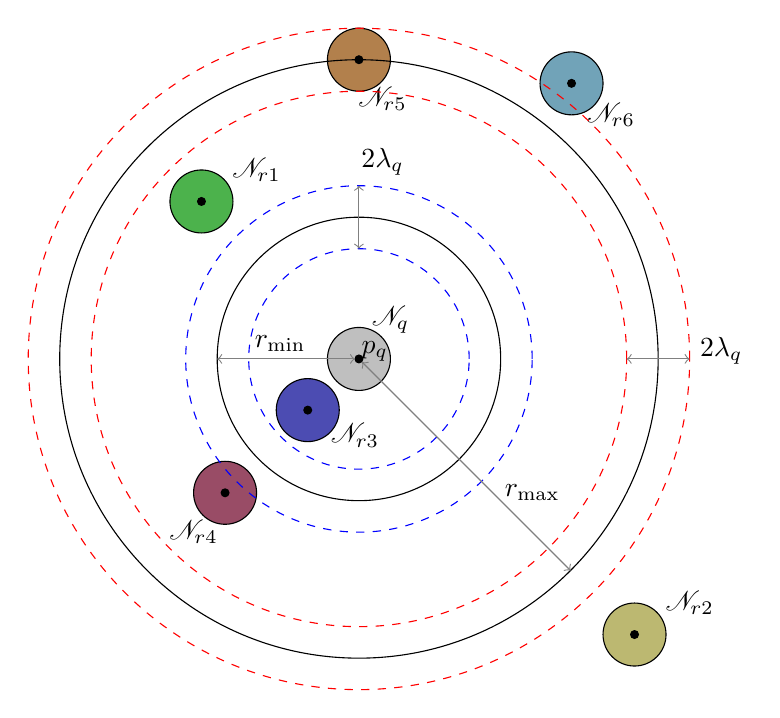
\begin{tikzpicture}
  % N_q
  \draw [fill=lightgray] (0, 0) circle (0.4);
  \node [ ] at (0.4, 0.5) { $\mathscr{N}_q$ };

  % p_q
  \node [draw, circle, inner sep=1pt, fill] at (0, 0) { };
  \node [ ] at (0.2, 0.1) { $p_q$ };

  % N_{r1}
  \draw [fill=green!40!gray] (-2.0, 2.0) circle (0.4);
  \node [draw, circle, inner sep=1pt, fill] at (-2.0, 2.0) { };
  \node [ ] at (-1.3, 2.4) { $\mathscr{N}_{r1}$ };

  % N_{r2}
  \draw [fill=yellow!40!gray] (3.5, -3.5) circle (0.4);
  \node [draw, circle, inner sep=1pt, fill] at (3.5, -3.5) { };
  \node [ ] at (4.2, -3.1) { $\mathscr{N}_{r2}$ };

  % N_{r3}
  \draw [fill=blue!40!gray] (-0.65, -0.65) circle (0.4);
  \node [draw, circle, inner sep=1pt, fill] at (-0.65, -0.65) { };
  \node [ ] at (-0.05, -0.97) { $\mathscr{N}_{r3}$ };

  % N_{r4}
  \draw [fill=purple!40!gray] (-1.7, -1.7) circle (0.4);
  \node [draw, circle, inner sep=1pt, fill] at (-1.7, -1.7) { };
  \node [ ] at (-2.1, -2.2) { $\mathscr{N}_{r4}$ };

  % N_{r5}
  \draw [fill=orange!40!gray] (0, 3.8) circle (0.4);
  \node [draw, circle, inner sep=1pt, fill] at (0, 3.8) { };
  \node [ ] at (0.3, 3.3) { $\mathscr{N}_{r5}$ };

  % N_{r6}
  \draw [fill=cyan!40!gray] (2.7, 3.5) circle (0.4);
  \node [draw, circle, inner sep=1pt, fill] at (2.7, 3.5) { };
  \node [ ] at (3.2, 3.1) { $\mathscr{N}_{r6}$ };

  % l
  \draw (0, 0) circle (1.8);
  % l - \lambda_q
  \draw [blue, dashed] (0, 0) circle (1.4);
  % l + \lambda_q
  \draw [blue, dashed] (0, 0) circle (2.2);

  % u
  \draw (0, 0) circle (3.8);
  % u - \lambda_q - \lambda_r
  \draw [red, dashed] (0, 0) circle (3.4);
  % u + \lambda_q + \lambda_r
  \draw [red, dashed] (0, 0) circle (4.2);

  % line from p_q to l
  \draw [gray, arrows=<->] (-0.05, 0) -- (-1.8, 0);
  \node [ ] at (-1.0, 0.2) { $r_{\min}$ };

  % line from p_q to u
  \draw [gray, arrows=<->] (0.04, -0.04) -- (2.687, -2.687);
  \node [ ] at (2.2, -1.7) { $r_{\max}$ };

  % line indicating u shell
  \draw [gray, arrows=<->] (4.2, 0) -- (3.4, 0);
  \node [ ] at (4.6, 0.1) { $2\lambda_q$ };

  % line indicating l shell
  \draw [gray, arrows=<->] (0, 2.2) -- (0, 1.4);
  \node [ ] at (0.3, 2.5) { $2 \lambda_q$ };

\end{tikzpicture}

%\caption{The shape of geometry to come.}
%\label{fig:rs_shapes}
%\end{centering}
%\end{figure}

%Figure \ref{fig:rs_shapes} details the possibilities when a particular
%combination is visited.

%\begin{enumerate}
%\item If the reference node is entirely contained in the range $[l +
%\lambda_q, u - \lambda_q]$ (as in $\mathscr{N}_{r1}$), then every
%descendant point of the reference node will be in the results for every
%descendant point of the query node; these can be added and then the combination
%can be pruned.\footnote{Because we have assumed that each query point will have
%$O(1)$ results, the total runtime of this step for each query node is $O(1)$, or
%$O(N)$ during the whole algorithm.  We will not consider the runtime
%contribution of this situation further, because other factors will outweigh
%this.}

%\item If the reference node is not contained at all in the range $[l -
%\lambda_q, u + \lambda_q]$ (as in $\mathscr{N}_{r2}$ and
%$\mathscr{N}_{r3}$), then no descendant points of the reference node will be in
%the results for any descendant point of the query node; thus, the combination
%can simply be pruned.

%\item If the reference node overlaps with the ranges $[l - \lambda_q,
%l + \lambda_q]$ or $[u - \lambda_q, u + \lambda_q]$ (as in
%$\mathscr{N}_{r4}$, $\mathscr{N}_{r5}$, and $\mathscr{N}_{r6}$), the node
%combination cannot be pruned by \texttt{Score()}, and must be descended.  This
%is the interesting case that we will focus on hereafter.  Only combinations of
%this type will make up the reference nodes in $|R_r^*|$.
%\end{enumerate}

%In the last situation, a reference node $\mathscr{N}_r$ with center $p_r$ and
%furthest descendant distance $\lambda_r$ satisfies at least one of the following
%two conditions:

%\begin{eqnarray}
%p_r &\in& B_{S_r}(p_q, u + \lambda_q + \lambda_r) \setminus B_{S_r}(p_q, u -
%\lambda_q - \lambda_r), \\
%p_r &\in& B_{S_r}(p_q, l + \lambda_q + \lambda_r) \setminus B_{S_r}(p_q, l -
%\lambda_q - \lambda_r).
%\end{eqnarray}

%Assuming first that $l - \lambda_q - \lambda_r > 0$, the reference node lies in
%the outer shell of a ball.  This is true of any $\mathscr{N}_r \in R_r$ for any
%cover set $R_r$ during the traversal.  If we can bound the size of the set

%\begin{equation}
%\left(B_{S_r}(p_q, u + \lambda_q + \lambda_r) \setminus B_{S_r}(p_q, u -
%\lambda_q - \lambda_r) \right) \cup \left(B_{S_r}(p_q, l + \lambda_q +
%\lambda_r) \setminus B_{S_r}(p_r, l - \lambda_q - \lambda_r) \right)
%\end{equation}

%\noindent then we will have bounded $| R_r^* |$.  First, observe that $\lambda_q
%+ \lambda_r \le 2^{s_r^{\max} + 1}$; then, the following algebraic
%manipulations lead us to our result.

%\begin{cor}
%In the monochromatic case ($S_q = S_r$, and $c_r = c_{qr} = c$), the
%running time of range search or range count is bounded by $O(c^{8 + \beta} N)$.
%\end{cor}

In this setting we can more easily consider the relation of the running time to
$\alpha$.  Consider $\alpha = (1 / 3)$; this yields a running time of $O(c^8 (N
+ \theta))$.  $\alpha = (1 / 7)$ yields $O(c^9 (N + I_t(\mathscr{N}_q +
\theta))$, $\alpha = (1 / 15)$ yields $O(c^{10} (N + I_t(\mathscr{N}_q) +
\theta))$, and so forth.  As $\alpha$ gets smaller, the exponent on $c$ gets
larger, and diverges as $\alpha \to 0$.

For reasonable runtime it is necessary that the $\alpha$-expansion of $S_{\max}$
be bounded.  This is because the dual-tree recursion must retain reference nodes
which may contain descendants in the range set $S[p_q]$ for some query $p_q$.
The parameter $C$ of the $\alpha$-expansion allows us to bound the number of
reference nodes of this type, and if $\alpha$ increases but $C$ remains small
enough that Corollary \ref{cor:rs} applies, then we are able to obtain tighter
running bounds.

%The assumption that on number of points in the range of $[(1 - \alpha)l, (1 +
%\alpha)u]$ for a single query is not too restrictive, but must be satisfied for
%the result to be meaningful.  After all, if that assumption is not satisfied,
%then it is not possible to perform range search in $O(1)$ time for each query
%point, making an $O(N)$ bound for the whole query set impossible.

%To show where the assumption is valid, consider that when presented with a very
%large dataset, a practitioner may perform monochromatic range search on a range
%$[l, u]$ for a geometric subset of their data; for instance, a hypersquare
%with side length $2u$.  This might be done in order to find a range $[l, u]$
%that produces a manageable number of results (if the range is too large, the
%number of results returned for each query point may be enormous).  Then, that
%practitioner may scale to a larger dataset by simply increasing the size of
%their hypersquare.  In this setting, the number of points in the range of
%$[(1 - \alpha)l, (1 + \alpha)u]$ for a single query remains $O(1)$ with respect
%to $N$.  Alternately, it should be possible to tighten the range $[l, u]$ as $N$
%increases in such a way that the number of points in the range remains constant.

%In cases where this assumption is not thought to be valid, it is straightforward
%to prove a bound on the running time of range search or range count by using the
%aspect ratio of the data, as in \cite{curtin2014kernel}.  However, the aspect
%ratio is particularly sensitive to datasets that have arbitrarily close points,
%and it is difficult to make assumptions about the aspect ratio.

%Alternately, if the assumption is not valid but it can be shown that the number
%of points in the range $[(1 - \alpha)l, (1 + \alpha)u]$ is $O(k)$ where $k$ has
%some dependence on $N$, then the running time can be easily bounded as $O(c^{4 +
%\beta} k(N + \theta))$.

%Also, note that the proof considers points with distance from $p_q$ in
%the range $[l + \lambda_q + \lambda_r, u - \lambda_q - \lambda_r]$; however, the
%pruning rule could also prune points that lie entirely in the range $[l, u]$ for
%additional speedup (Algorithm \ref{alg:rs_sc} does not do this because there is
%no theoretical benefit in our proof).  Unfortunately, the expansion constant
%does not make working with slices of balls easy, and as a result the runtime
%bound as given is likely to be loose when this additional prune is made,
%especially when $u - l$ is large.


%\section{Range Search with Aspect Ratio}

%In this section, we will bound the running time of range search in a different
way, by using the aspect ratio of the reference set $S_r$.

Define $\tau_r$ to be the aspect ratio of the reference set $S_r$, which is the
largest distance between any two points in $S_r$ (denote this quantity as
$\gamma_r$) divided by the smallest nonzero distance between any two points in
$S_r$ (denote this quantity as $\delta_r$).

\begin{thm}
Under the standard assumptions and given a reference set aspect ratio of
$\tau_r$, using the range search \texttt{BaseCase()} and \texttt{Score()} as
given in Algorithms \ref{alg:rs_bc} and \ref{alg:rs_sc}, respectively, with a
search range of $[l, u]$, and also assuming that the length of the list of
results for each query point in $S_q$ is $O(1)$, the running time of range
search or range count is bounded by

\begin{equation}
\begin{split}
  O((1 + \tau_r) c_r^{7 + \log_2 c_r} \nu N),& \text{\ \ \ \ if } u \ge \gamma_r\\
  O((1 + \frac{u}{\gamma_r} \tau_r) c_r^{7 + \log_2 c_r} \nu N),&
\text{\ \ \ \ otherwise}.
\end{split}
\end{equation}

\end{thm}

\begin{proof}
As in the previous proof, we know that the running time of \texttt{BaseCase()}
and \texttt{Score()} are $O(1)$, and that the runtime of the algorithm is
bounded by $O(c_r^4 \nu |R^*| N)$.  Thus, again, our goal is to bound the
maximum size of the reference set $| R^* |$.

From Equation \ref{eqn:rsballs}, we can ignore the inner ball term to see that

\begin{equation}
|R^*| \le \left| B_{S_r}(p_q, u + 2^{s_r^{\max} + 1}) \cap C_{s_r^{\max}}
\right|.
\end{equation}

It is true that $|B_{S_r}(p_r, \gamma_r)| = N$ for all $p_r \in S_r$; also, if
$u \ge \gamma_r$, then $B_{S_r}(p_r, u) = B_{S_r}(p_r, \gamma_r)$.  Thus, define
the auxiliary quantity $\zeta_r = \min (u, \gamma_r)$.  Using this auxiliary
quantity, we can now employ a packing argument, as in previous proofs.  For any
$p_r \in P$,

\begin{eqnarray}
|B_{S_r}(p_q, u + 2^{s_r^{\max} + 1})| &\le& |B_{S_r}(p_q, \zeta_r +
2^{s_r^{\max} + 1})| \\
 &\le& |B_{S_r}(p_q, (1 + \frac{\zeta_r}{2^{s_r^{\max} + 1}}) 2^{s_r^{\max} +
1})| \\
 &\le& |B_{S_r}(p_r, (1 + \frac{\zeta_r}{2^{s_r^{\max} + 1}}) 2^{s_r^{\max} +
2})| \\
 &\le& c_r^{3 \log_2{(1 + \zeta_r / 2^{s_r^{\max} + 1})}} | B_{S_r}(p_r,
2^{s_r^{\max} - 1})|.
\end{eqnarray}

The total number of nodes in $R$ is bounded by the number of disjoint balls of
size $2^{s_r^{\max} - 1}$ that can be packed into a ball of radius $(1 + \zeta_r
/ 2^{s_r^{\max} + 1}) 2^{s_r^{\max} + 2}$.  In the worst case, this packing is
perfect, and we have that

\begin{equation}
\left| B_{S_r}(p_q, \zeta_r + 2^{s_r^{\max} + 1}) \cap C_{s_r^{\max}} \right|
\le
\frac{| B_{S_r}(p_r, (1 + \zeta_r / 2^{s_r^{\max} + 1}) 2^{s_r^{\max} + 2}) |}{|
B_{S_r}(p_r, 2^{s_r^{\max} - 1}) |} \le c_r^{3 \log_2{(1 + \zeta_r /
2^{s_r^{\max} + 1})}}.
\end{equation}

We can simplify the last term:

\begin{equation}
c_r^{3 \log_2(1 + \zeta_r / 2^{s_r^{\max} + 1})} = (1 +
\frac{\zeta_r}{2^{s_r^{\max} + 1}}) c_r^{3 \log_2 c_r}.
\end{equation}

In the worst case, $s_r^{\max}$ is the bottom level of the tree, and
$2^{s_r^{\max}}$ is the distance between the two closest points in $S_r$ (call
this distance $\delta_r$).  Expand $\zeta_r$ to its definition to get the result
that

\begin{equation}
|R^*| =
\begin{cases}
  (1 + \tau_r) c^{3 \log_2 c},& \text{if } u \ge \gamma_r \\
  (1 + \frac{u}{\gamma_r} \tau_r) c_r^{3 \log_2 c_r},& \text{otherwise}.
\end{cases}
\end{equation}

\end{proof}

It is important to note that as $u$ decreases, the running time of the algorithm
also decreases accordingly.

Possibilities for improvement:

\begin{itemize}
  \item Can we use a packing argument to bound the number of balls in a `slice'?

  \item Can we incorporate the lower bound $l$ into the proof to subtract large
parts away?

  \item Can we modify the \texttt{Score()} rules for pruning when a node is
entirely contained within the range, and then only consider slices of size
$2^{s_r^{\max} + 1}$ centered at radius $u$ and $l$?
\end{itemize}

The second two ideas depend on the first idea.


%\section{Empirical investigations}
%\label{sec:emp}

%In the previous section we have expressed a number of bounds of roughly the form

\begin{equation}
O(c^a (N + \theta))
\end{equation}

\noindent for some $a$.  Although both $c$ and $\theta$ are well-defined and
straightforward, there is limited practical utility to these bounds without
empirical experimentation.  One can easily say `these algorithms scale linearly
if $c$ has no dependence on $N$ and $\theta$ is not superlinear in $N$'; this is
useful.  But this does not answer the question of `on what datasets are these
assumptions valid, and how do these algorithms actually perform in practice?'

To help answer this oft-overlooked query, we perform an empirical analysis of
$c$, $i_t(\mathscr{T}_q)$, and $\theta$ on a variety of different datasets for
each algorithm we have presented.

\subsection{The expansion constant $c$}

\subsection{Tree imbalance $i_t(\mathscr{T})$}

\subsection{Nearest neighbor search}

\subsection{Kernel density estimation}

\subsection{Range search}


\section{Conclusion}
\label{sec:conclusion}

We have presented a unified framework for bounding the runtimes of dual-tree
algorithms that use cover trees and the standard cover tree pruning dual-tree
traversal (Algorithm \ref{alg:cover-tree-dual}).  Our main result, Theorem
\ref{thm:ct-runtime}, allows plug-and-play runtime bounding of these algorithms.
We have shown that Theorem \ref{thm:ct-runtime} is useful for bounding the
runtime of nearest neighbor search (Theorem \ref{thm:nns}), approximate kernel
density estimation (Theorem \ref{thm:kde-bound}), exact range count, and exact
range search (Theorem \ref{thm:rs}).  With our contribution, bounding a cover
tree dual-tree algorithm is straightforward and only involves bounding the
maximum size of the reference set, $| R^* |$.


%\bibliographystyle{plain}
\bibliography{bounds}

% Appendix doesn't have anything useful or non-straightforward.
%\appendix
%\section{Expansion Constant Properties}

I talked to someone who wasn't convinced that all of the following useful lemmas
were true, so I went out and proved them.  Now I've typeset them.

\begin{lemma}
\label{lem:ec_rec}
Given an expansion constant $c$ as defined in Definition \ref{def:int_dim}, for any
ball $B_S(p, 2^i \Delta)$ where $p \in S$, $i \in \mathbb{N}$, $\Delta > 0$,

\begin{equation}
| B_S(p, 2^i \Delta) | \le c^i | B_S(p, \Delta) |.
\end{equation}
\end{lemma}

\begin{proof}
This follows from $i$ recursive applications of the definition of the expansion
constant.
\end{proof}

\begin{lemma}
\label{lem:ec_re}
Given an expansion constant $c$ as defined in Definition \ref{def:int_dim}, for any
ball $B_S(p, \alpha \Delta)$ where $p \in S$, $\alpha \in \Real$, $\alpha \ge 1$,
$\Delta > 0$,

\begin{equation}
| B_S(p, \alpha \Delta) | \le c^{\log_2 \alpha} | B_S(p, \Delta) |.
\end{equation}
\end{lemma}

\begin{proof}
By Definition \ref{def:int_dim} and Lemma \ref{lem:ec_rec}, it is obvious that
the statement holds when $\alpha \in \mathbb{N}$.  However, the definition of
expansion constant makes no particular bound on the number of points added when
the ball is not doubled but simply increased by some real factor.  We will
perform this proof by contradiction.

Assume that there exists some $\alpha \in \mathbb{R}$ where $\alpha > 1$ and

\begin{equation}
| B_S(p, \alpha \Delta) | > c^{\log_2 \alpha} | B_S(p, \Delta) |.
\end{equation}

By Definition \ref{def:int_dim}, we also know that

\begin{equation}
| B_S(p, \alpha \Delta) | \le c | B_S(p, (\alpha / 2) \Delta) |.
\end{equation}

Combining these two equations gives that

\begin{equation}
c | B_S(p, (\alpha / 2) \Delta) | > c^{\log_2 \alpha} | B_S(p, \Delta) |
\end{equation}

\noindent or alternately

\begin{equation}
c^{(1 - \log_2 \alpha)} | B_S(p, (\alpha / 2) \Delta) | > | B_S(p, \Delta) |.
\end{equation}

First, assume that $\alpha < 2$.  Then, $|B_S(p, (\alpha / 2) \Delta)| \le
|B_S(p, \Delta)|$.  Thus,

\begin{equation}
c^{(1 - \log_2 \alpha)} | B_S(p, \Delta) | > | B_S(p, \Delta) |
\end{equation}

\noindent which is a contradiction because $c^{(1 - \log_2 \alpha)} > 1$.

Now, assume that $\alpha > 2$.  Define $\beta = 2^i \alpha$ where $i \in
\mathbb{N}$ is such that $1 < \beta < 2$.  Then,

\begin{equation}
| B_S(p, (2^i \beta / 2) \Delta) | \le c^i | B_S(p, (\beta / 2) \Delta) |.
\end{equation}

Because $\beta < 2$, $|B_S(p, (\beta / 2) \Delta)| \le |B_S(p, \Delta)|$.  Thus,

\begin{equation}
|B_S(p, (2^i\beta / 2) \Delta)| \le c^i | B_S(p, \Delta) |.
\end{equation}

From earlier, this implies that

\begin{equation}
\label{eqn:contr}
(c^{(1 - \log_2 (2^i \beta))}) (c^i) |B_S(p, \Delta) | > |B_S(p, \Delta) |.
\end{equation}

Note that $(c^{(1 - \log_2 (2^i \beta))}) (c^i) = c^{(1 - \log_2 \beta)}$, which
is greater than $1$ because $\beta < 2$.  This means that Equation
\ref{eqn:contr} is a contradiction, and thus, for all $\alpha \in \mathbb{R}$,
the statement of the lemma holds.
\end{proof}

\begin{lemma}
\label{lem:ec_neg}
Given an expansion constant $c$ as defined in Definition \ref{def:int_dim}, for
any ball $B_S(p, 2^{-i} \Delta)$ where $p \in S$, $i \in \mathbb{N}$, $\delta >
0$,

\begin{equation}
|B_S(p, 2^{-i} \Delta)| \ge c^{-i} |B_S(p, \Delta)|.
\end{equation}
\end{lemma}

\begin{proof}
Observe that $|B_S(p, \Delta)| \le c^i |B_S(p, 2^{-i} \Delta)|$.  Simple
algebraic manipulation yields the result.
\end{proof}

\begin{lemma}
Given an expansion constant $c$ as defined in Definition \ref{def:int_dim}, for
any ball $B_S(p, \alpha \Delta)$ where $p \in S$, $\alpha \in \mathbb{R}$,
$0 < \alpha \ge 1$, $\delta > 0$,

\begin{equation}
|B_S(p, \alpha \Delta)| \ge c^{\log_2 \alpha} |B_S(p, \Delta)|.
\end{equation}
\end{lemma}

\begin{proof}
(idea) This is a relatively straightforward combination of the proofs of
Lemmas \ref{lem:ec_neg} and \ref{lem:ec_re}.
\end{proof}

Two important observations:

\begin{itemize}
  \item We can place an upper bound on the number of points added as a ball
grows an arbitrary amount.

  \item We can place a lower bound on the number of points removed as a ball
shrinks an arbitrary amount.
\end{itemize}


\end{document}
